\documentclass[12pt,english]{report}

% % % These packages imported by Abe
\usepackage{xargs} 
%has to load before umlthesistemplate
\usepackage[colorinlistoftodos,prependcaption,textsize=tiny]{todonotes}
\newcommandx{\unsure}[2][1=]{\todo[linecolor=red,backgroundcolor=red!25,bordercolor=red,#1]{#2}}
\newcommandx{\change}[2][1=]{\todo[linecolor=blue,backgroundcolor=blue!25,bordercolor=blue,#1]{#2}}
\newcommandx{\info}[2][1=]{\todo[linecolor=OliveGreen,backgroundcolor=OliveGreen!25,bordercolor=OliveGreen,#1]{#2}}
\newcommandx{\improvement}[2][1=]{\todo[linecolor=purple,backgroundcolor=purple!25,bordercolor=purple,#1]{#2}}
\newcommandx{\thiswillnotshow}[2][1=]{\todo[disable,#1]{#2}}

%Has to load before umlthesistemplate
\usepackage{auto-pst-pdf}

%Can probably load anytime, but seems to work in advance...
\usepackage{graphviz}
\usepackage{microtype}
\usepackage{enumitem}
\usepackage{multicol}
\usepackage{caption}
\usepackage{subcaption}
\usepackage{relsize}

%For BNF
\usepackage{backnaur}

\usepackage[toc,page]{appendix}
% From https://tex.stackexchange.com/questions/163330/creating-figures-to-show-binary-values
%For showing bitfields in the control hardware
\usepackage{bytefield}
\newcommand{\colorbitbox}[3]{%
\rlap{\bitbox{#2}{\color{#1}\rule{\width}{\height}}}%
\bitbox{#2}{#3}}
\definecolor{lightcyan}{rgb}{0.84,1,1}
\definecolor{lightgreen}{rgb}{0.64,1,0.71}
\definecolor{lightred}{rgb}{1,0.7,0.71}
% % % End Abe's stuff

\usepackage{umlthesistemplate}

\title{Command Language for Single-User, Multi-Robot Swarm Control}
\author{Abraham M. Shultz}
\pastdegrees{B.S. Worcester Polytechnic Institute (2004) \and M.S. University of Massachusetts Lowell (2014)}
\degree{Doctor of Philosophy}
\department{Computer Science}
\university{University of Massachusetts Lowell}
\majorprofessor{Dr. Holly A. Yanco}
\majorproftitle{Dissertation Chair}
\members{Dr. Radhika Nagpal \and Dr. Jay McCarthy}
\date{ 3 December, 2018}

\includeapproval
%Uncommenting any of these breaks the \begin{document} lines
\abstract{Command and control systems designed for a single operator to operate a single robot do not scale to control of swarms \citep{WangSearchScale}. User interfaces that require the user to attend to each robot overwhelm the controller when the number of robots increases beyond 12 or 13 for uncrewed aerial vehicles (UAVs) and 3-9 for uncrewed ground vehicles (UGVs) \citep{WangSearchScale}. As robot swarms increase beyond these bounds, the control system must shift to from controlling individual robots to controlling the swarm as a single entity or set of groups. However, the form this interface should take to permit easy and understandable control of the swarm is largely undefined.

Previous work in human-robot interaction (HRI) shows that multi-touch interfaces allow a scalable and direct mapping between the desires of the user and sequences of commands to robots \citep{micire2009multi}. By defining a mapping from user interface gestures to individual programs loaded on each robot, we can allow an individual to control arbitrarily large, heterogeneous swarms. This thesis presents an interface that extends previous work on multitouch interfaces for small groups of robots to larger swarms, and automates the process of converting command gestures into programs for each robot. The use of individual control programs rather than centralized control is important to realize the potential of swarms to continue to operate despite the possible failure of individual swarm robots.

The contributions of this thesis are a new swarm hardware platform, software to support it, and a user interface that converts user commands into programs for each robot in the swarm. 
The new swarm platform initially combined a wifi-enabled microcontroller with commodity mobility platforms sourced from children’s toys to allow large swarms to be built at a low cost. 
While children's toys ultimately were not sufficiently reliable to serve as mobility platforms, the design of the controller was not bound to a specific mobility platform, and so was applied to 3-D printed mobility platforms. 
In order to maintain the low cost, sensors for the swarm robots were simulated with a top down camera. 
The use of simulation allows individual swarm members to be constructed cheaply in the present, while leaving the path clear in the future to push computation to the individual members as computer hardware becomes cheaper and smaller.
}

\acknowledgments{ Thank you to Dr. Holly Yanco, for encouraging me to turn one of my side projects into a dissertation, for providing guidance and resources for all these years, and finally for the encouragement to get out. Your ceaseless work to run the Robotics Lab and the NERVE Center and encourage a good mixture of freedom and focus for the people working there have made it a fantastic place to work. 

Thank you to Dr. Jay McCarthy for the useful pointers in programming languages and verification, and for keeping me on track when I was getting into the weeds of Turing completeness. 

Thank you to Dr. Radhika Nagpal for the loan of the E-Pucks, and for an impressive body of work in swarm robotics that inspired and informed some of this work. 

Thank you to Jonathan Roche for vastly speeding up the virtual laser, to James Kuczynski and Dalton Curtin for their attention to detail in coding the user responses, and everyone else in the UML robotics lab that I've asked to read papers, write ROS modules, or otherwise help out. Collaboration is one of our lab's strengths, keep it that way when I'm gone.  

Thank you to my parents, for teaching me, for encouraging me to pursue my own education, and putting up with the huge piles of messed-about-with hardware that follow me around. Your unconditional love and support has been a comfort to me in times of stress, and a joy always.

%Thank you to Vanessa Evers, Edwin Dertien, and the staff of the Human Media Interaction group at the University of Twente for hosting me while I worked on the swarm hardware. It was engaging and inspiring to ``do things with stuff'' with you. 
 }
\includetoc 
\maketitle

\begin{document}

\clearpage

% !TeX root = ams_thesis.tex
\chapter{Introduction}
\thispagestyle{fancy}

Methods for command and control that are based on issuing individual orders to individual robots do not scale to large numbers of robots \citep{WangSearchScale}.
By defining a mapping from user interface gestures to individual programs loaded on each robot, we can allow an individual to control arbitrarily large, heterogeneous groups of robots.
% Previous work in HRI shows that multi-touch interfaces allow a scalable and direct mapping between the desires of the user and sequences of commands to the swarm \cite{micire2009multi}. 
While swarm hardware is not yet at a point where very complex computation may be pushed directly to the swarm nodes themselves, that time is not far off. 
Indeed, some systems already have moderately powerful computers, but at fairly high cost for each the individual robots \citep{millard2017pi}.

Until computational power in the individual swarm units reaches the levels required for complex computation, virtualization of computing resources can provide an adequate test environment for the development of swarm control algorithms at modest requirements in terms of space and power consumption. 
Centralizing the control of a single swarm of robots makes the system as a whole sensitive to the failure of the central controller. 
To avoid this type of failure, the overall action of the swarm should be guided by decentralized emergent behavior, rather than centralized orchestration. 
Each robot receives its own program, and the sum of the execution of the programs on each robot results in the completion of the swarm's task.
The various approaches to the development of swarm robot control programs show that a wide variety of approaches can still result in robust controllers for swarm robots. 
However, placing bounds on the sensing ability and communication ability of the robots has substantial effects on the programs that can be developed for them. 

\section{Problem Statement} \label{section:Problem_Statement}

One potential method to control a swarm of robots is having a central computer dictate to individual robots how the robots should move.
However, centralized control is only as robust as the central controller and its connection to the robots. 
Distributed control systems do not have a single point of failure as centralized models do. 
In order to create reliable and useful swarm robotic systems, users must be able to specify a desired end state of the system to which the swarm can converge without reliable orchestration from a central controller. 
Moreover, this convergence must occur in the face of unreliability on the part of the individual swarm members. 

The current state of development of emergent control of swarms is guided by ad-hoc, iterative development models that are somewhat suited to software developers, but not suited for use by non-programming end users \citep{palmer2005behavioral}.
The motivating examples of uses for swarms are task oriented, such as sending swarm robots into disaster zones to search for survivors.
Iterative software development does not have the ability to adapt quickly enough in the face of changing situations in a disaster area, and software development training would be out of scope for first responders. Therefore, it is desirable to automate the construction of control software for a swarm so that it can adapt to a situation, without requiring significant development time. 
In order to support interactive control during a developing situation, the construction of the software should occur over a similar time scale to the user interactions.

Initially, part of the intent of this work was to determine if robot control programs could be developed to function under the following assumptions, which mirror some of the difficulties found in operation of robots under difficult field conditions. 

\begin{enumerate}
	\item Robots' sensing is limited in range. Because of this limitation and dynamic environments, the information that robots can have about distant points is limited. 
	\item Networking between robots is unreliable, due to range, limited power, and possible interference. It is not the case that any robot can reach any other robot at any time.
	\item Because of limits in sensing and networking, it may be the case that global, absolute localization is unavailable. 
	\item Robots can fail. Algorithms to control them should not depend on the perfect functioning of any individual robot. 
\end{enumerate}

Ultimately, while the resulting programs can operate under many of these conditions, the user interface (UI) design used in user experiment implies some form of localization for the robots.
For the study described in this work, the UI displays, on a multi-touch screen, a top-down view of the robots and their surroundings. 
Placing the robots in a map-like view relative to each other implies that the locations of the robots relative to each other can be determined. 
With this interface, the users were presented with a series of tasks, and could use any method they wished to command the robots to perform the task. 
Without metric localization, some of the tasks posed in the user experiments are possible, if certain aspects of the goals are relaxed. 


\section{Hypotheses} \label{section:Hypotheses}

\subsection{H1: User gestures change based on the size of the swarm}

It is hypothesized that there exists a number of robots beyond which users will transition from treating robots as individuals to interacting with the robots in small groups or as a single large group. 
As the user interacts with the multi-touch user interface, they will choose the gestures that they feel convey their intention to the system. 
The collected gestures for a particular user are their gesture set.
Across multiple users, the transition point will be apparent because of a change in the gesture set that the users choose to interact with the swarm. 
It is hypothesized that above the transition point, users will be more likely to neglect some subset of the available robots. 
The user will instead issue commands that control the bulk of the robots as a cloud or flock, but may leave some robots unused. 
For example, the user may switch from selecting robots as individuals to shaping and pushing the swarm the way a child might play with a bug, putting their hand down so the bug goes around or avoids it, touching the back of the bug gently to make it scurry forwards, and so forth, or by shaping the group as if sculpting, with pushing and pinching to ``carry'' groups around. 
The user may also change how they indicate which robots are to be interacted with. 
Rather than selecting each robot by clicking on it, they may ``paint'' over the area containing the robots they want to use, or draw a circle around them. 
The size of the swarm where changes in the user gestures occur will indicate the transition point between interacting with individual robots and interacting with the swarm as a whole. 
%Harriet \emph{et al}. also put the estimated transition point between multi-agent control and swarm around 50 individuals \citep{harriott2014biologically}.  
%Above that threshold, human interaction may be able to remain focused on macro level behavior, influencing the overall behavior of the swarm rather than control of individuals.
This hypothesis would be invalidated by the gestures selected by the user displaying no correlation with the size of the swarm that they are controlling. 


\subsection{H2: Changes in display of the swarm can change user behavior}

It is hypothesized that a display that obscures individual robots and displays a cloud or swarm boundary will cause the user to treat the swarm as a whole rather than individuals, which will be apparent because the user will use the same gestures they would use to control a single robot. 

Once the ratio of the size of individual swarm members to the size of the area the swarm is in becomes sufficiently large, displaying the swarm members at the same scale as the map will result in the representation of the swarm members being too small to interact with. 
This problem will arise at smaller scales if the swarm robots are themselves quite tiny, and some of the available swarm robots are indeed small \citep{pelrine2012diamagnetically}.
Scaling the representation of the robots up, relative to the map, will make the robot representations overlap unrealistically and obscure the map. 
Instead, we propose that for certain scales of swarms, it makes sense to represent the swarm as the area covered, rather than the locations of the individual robots.
This approach has been used successfully for navigation of a swarm of uncrewed aerial vehicles (UAVs) in three dimensions, by developing a controller that causes the individual UAVs to remain within a bounding prism, and allowing the user to control the shape and location of that prism \citep{ayanian2014controlling}.

This hypothesis would be invalidated by the gestures selected by the user in the single robot case being dissimilar from those selected in the case where the swarm is displayed as a cloud or covered region. 

\subsection{H3: User gestures can be converted to programs}

It is hypothesized that user commands on a multitouch display can be automatically converted into programs for each robot that will converge to the desired behavior. These programs will operate using only local sensing and local communications, and without resorting to global, absolute localization. 

Further, it is hypothesized that the user commands can be represented as a grammar that can be transformed into programs for each robot. 
These programs should result in the convergence of the swarm to the desired behavior using only local sensing and local communications, and without resorting to global, absolute localization. 
However, this hypothesis must be modified with a few caveats. 
First, under the assumption that robots can fail, it is possible that the entire behavior can fail. 
For example, if enough of the robots are incapacitated, it may be that not enough are left to complete the task. 
It's also possible that at compile time, the task is still possible, but a later change of the environment renders it impossible. 
Assessing whether or not a user-specified action will be completed is not possible for all of the usual reasons that prevent prediction of the future, but in some limited cases, it may be possible to determine whether a specified action is impossible. The goal of this work is to provide a best-effort attempt to satisfy the user command, rather than prove anything about the possibility of doing so. 
This hypothesis would be disproven by demonstration that a desired user action, as represented by control gestures on the user interface, could not be converted to a program that operates without global localization and that requires only local sensing and communication.

\subsection{H4: A cheap indoor swarm can be built with commodity hardware}

The Kilobots set a remarkably low price point for individual swarm robots, with the parts for each robot costing approximately \$15 \citep{rubenstein2014kilobot}. 
However, the Kilobots move by stick-slip locomotion, and so require a smooth, level surface to operate on. 
Children's toys, such as radio controlled (RC) toy cars, tanks, and legged ``insects'' are designed to operate on slightly more difficult terrain, and so could be used to extend swarm robotic experiments into natural indoor settings. 
In order to enable the control of toy mobility platforms as swarm robots, a common controller with the ability to adapt to various toys is needed.   
As computing hardware decreases in price and size, more and more ability can be built into smaller and smaller hardware. 
The development and popularity of smartphones has driven the development of smaller sensors and lower power processors, as well as thinner and smaller battery technology. 
As Internet of Things (IoT) technology becomes increasingly popular, it becomes easier and cheaper to add smaller and lower-power devices to communications networks. 
The parts that go into these consumer technologies are also made less expensive by economies of scale. 
Assuming a fixed set-up cost, the more finished devices are produced, the greater the amortization of the setup cost across the devices. 
Since IoT is expected to deliver connectivity for tens or hundreds of devices per end user, the expected economics drive down the cost of network connectivity.
As a consequence, by using components intended for IoT devices, cell phones, and similar consumer electronics, the cost of building small robots will also continue to drop.

This hypothesis would be disproved by a swarm robot capable of operating in a naturalistic indoor setting requiring more than twice the cost of a Kilobot in parts. 


% !TeX root = ams_thesis.tex
\chapter{Related Work}

\section{Overview of Previous Swarm Hardware} \label{section:Overview_of_Previous_Swarm_Hardware}

Swarm robots are generally small. 
The reason to keep swarm robots small is related to both the cost of making them and the cost of using them. 
Larger robots consume more materials per unit, and so cost more money.
As a result, for a given number of swarm units, larger robots will result in a higher cost swarm. 
Also, each robot requires some amount of space to move around in. 
To keep the ratio of free space to robots constant, the area of space used by the robots grows as the robots do. 
If the ratio isn't kept constant, the robots will crowd each other, and so large robots will require either a very large space, or become overly crowded.
Finally, larger robots are more cumbersome to deal with. 
They require larger storage areas, possibly teamwork to lift or repair, and so forth. 
All of these efforts are also multiplied by the number of robots in the swarm. 
 
In addition to budgetary constraints, interaction with an environment built for humans places an upper bound the scale of the individual swarm members. 
For example, typical indoor doorways are around thirty inches wide, so a robot would have to be less than thirty inches wide to fit through them. 
The lower bound on swarm robots is generally dictated by fabrication technology, with smaller robots becoming increasingly difficult to assemble. 
As a result of these bounds, swarm robots are mostly between 1cm$^3$ and 0.3m$^3$. 
This scale range divides fairly evenly into robots that can operate in large swarms on a table, and those that can operate in swarms within a room, albeit possibly a large room. 
The challenge of construction of swarm robot hardware, then, is to put all of the same parts as non-swarm mobile robots: a mobility platform, a power supply, a processor, some sensors, and a communication system, into a small package.
Many impressive designs for small swarm robot platforms have been proposed and constructed as part of research in swarm robotics. 
However, most of these platforms are no longer easily commercially available, or never were. 

\subsection{Tabletop Swarms} \label{section:Tabletop_Swarms}

At the low end, in terms of size, the I-SWARM Project was intended to create a 2x2x1mm robot that moved by stick-slip locomotion actuated by piezo levers \citep{seyfried2005swarm}. 
Over the course of the project from 2004-2008, the hardware was developed and used in research, but was not converted to a commercial product.
Other techniques have been developed to use magnetic fields to apply force to small magnetic objects, resulting in controlled motion of the objects \citep{floyd2008untethered, pelrine2012diamagnetically}.
These systems are not amenable to decentralized control, because the moving components are not themselves robots. 
The moving parts are more accurately viewed as manipulators, with the instrumented environment, any sensors for feedback from that environment, and the manipulators themselves comprising a single robot. 

Early small-scale swarm robots were based on microprocessors, and were primarily research platforms for the groups that developed them, rather than commercially available products.
Alice, by Caprari \emph{et al}. combined a PIC16F84 processor, motors, RF and IR networking, and enough battery power for 10 hours of autonomy into a robot measuring under 2.5cm$^3$ \citep{caprari1998autonomous}. 
The Jasmine swarm robots were possibly the closest thing to a commercially-available successor to Alice \citep{kernbach2011swarmrobot}.
Jasmine measured 26x26x20mm, and included an ATMega processor, IR close range communication and obstacle detection, two motor skid steering, and lithium-polymer batteries.
Jasmine units cost about 100 Euro (\$111 USD) each when they were available, and they are no longer available for purchase. 
InsBot was a small robot, measuring 41mm x 30mm x 19mm, that was designed to interact with cockroaches \citep{colot2004insbot}.
It used two processors, one to run higher level behaviors and one to interface with a suite of sensors that included 12 IR sensors and a linear camera. 
The AmIR robot measured 6.5cm in diameter and 6cm tall. It has a more modern processor than Alice \citep{arvin2009development}.
There is no evidence that AmIR was ever widely available, and it cost \pounds65, or \$92 USD per unit \citep{arvin2015colias}.
The successors to Amir, Colias and the related Colias-$\Phi$, are dual-microprocessor systems similar to Jasmine in functionality, but with additional features for pheromone robotics applications \citep{arvin2014colias, arvin2015colias}. 
Colias is built out of two PCBs, with the upper PCB and processor handling IR collision avoidance and communication, and the lower processor controlling the motors, power management, and a few other sensors.
Colias robots cost \pounds25, or \$35US, in parts, but are not commercially available. 
The Colias-$\Phi$ model has an even more impressive price, at \pounds16, or \$22 USD.

Even when they are commercially available, most existing swarm robots are too expensive to build a large swarm.
The E-puck from EFPL is approximately 800 Swiss francs (\$810 USD) per unit, so the cost of maintaining a large swarm can become daunting quickly. 
The high price of the E-puck is a result of its extensive suite of sensors, including a camera and 360$^{\circ}$ IR range sensor and communication system. 

The r-one research robot is cheaper than the E-puck, at approximately \$220 USD per unit \citep{mclurkin2013low}. 
The developers of the r-one position it as a more-featureful and less expensive alternative to the E-puck (\$810, cannot sense neighbors without additional hardware), Parallax's Scribbler (\$198, minimal sensors), the iRobot Create (\$220, requires additional hardware to be programmable), the K-team Khepera III (\$2000), and the Pololu 3pi (\$99, minimal sensors). 

The Harvard Kilobots are a more recent entry to inexpensive swarms, and have been produced in large quantities \citep{rubenstein2014kilobot}. 
Kilobots contain about \$15 worth of parts. 
However, this cost ignores the effort of assembling the robots. 
A 10-pack of assembled Kilobots sells for 1100 Swiss francs, or about \$112 (US) per robot. 
The Kilobots are intended for research in a highly homogeneous environment, with most or all of the robots executing the same program. 
As a result, they are designed to be programmed in parallel using an IR interface. 
For small groups, individual Kilobots can be programmed differently, but any attempt to give each of a very large collection of robots an unique program will take a long time. 
The Kilobots also move by stick-slip motion, and so must operate on a smooth surface, such as a whiteboard. 

The GRITSBots platform is a differential-drive platform using stepper motors \citep{pickem2015gritsbot}.
GRITSBots use the same processor as Colias, in a similar configuration, with one processor operating sensors and the other controlling the robot's motors. 
The sensor board incorporate a 3D accelerometer and gyro as well as a 6-direction IR distance sensing ring. 
GRITSBots measure 31mm x 33mm, and cost approximately \$50 for parts per unit. 

The Psi Swarm robot is a 10cm diameter round robot with proximity sensing, a compass, bluetooth wireless connectivity, and autonomous charging via ground contacts \citep{hilder2016psi}.
As with many of the platforms described in this section, it is not commercially available, but the designs to have the circuit boards fabricated and the body 3D printed are freely available. 

MROBerTO is a swarm robot with a 16mm$^2$ footprint. It has modular expandability via a header for daughterboards, and includes a single-point laser rangefinder, gyro, accelerometer, compass, and a VGA resolution camera \citep{Kim2016mROBerTOAM}. 
The mROBerTO processor is a 32-bit ARM processor with Bluetooth and ANT+ wireless. 
All of this hardware is only \$60 per unit in quantities of 25 or more units. 
In order to permit an overhead camera to localize the mROBerTO robots, a single RGB LED on top of the camera can be lit in a unique color to localize the robot, and a green LED on the front of the robot indicates its heading. 
The use of color information is likely much faster to process than fiducual tags, but does have the disadvantage that it is only useful in 2D unless a stereo camera is used. 

The Zooids of Le Goc \emph{et al.} are interesting in that the robots themselves are positioned as both a physical interface and a swarm \citep{le2016zooids}. 
They are designed to be used as physical controls, such as knobs or sliders, as well as being able to move themselves.
The individual robots measure 2.6cm in diameter, and localize themselves using a projected grey coded light signal from a high-speed projector. 
The authors estimate the individual cost of a Zooid at around \$50. 

Swarm robots have also been developed for aquatic and aerial robotics as well, although the problems unique to those domains are outside of the scope of this work \citep{costa2016design, preiss2017crazyswarm}. 
It is worth noting that the Crazyflie quadcopter platform on which the Crazyswarm is based is a commercial product, and so available to everyone. 
At least one legged, inexpensive robot platform has also been proposed as a swarm platform, but no swarm composed of them appears in the literature \citep{kalat2015tribot}. 

One way to reduce the cost of swarm robots is to use commercial, off-the-shelf (COTS) hardware in the construction of the robot. 
Reusing existing hardware leverages the economies of scale that reduce the price of commercial hardware, as well as eliminating the need to design or build the COTS parts. 
Use of COTS parts in research robotics has led to at least two platforms referred to as COTSBots \citep{bergbreiter2003cotsbots, soule2011cotsbots}.
The first COTSBots used mote hardware for the communications link and sensing, plus a motor control add-on board \citep{bergbreiter2003cotsbots}. 
The mobility platform is a modified toy, in particular, a specific brand of high-quality micro RC car.
At the time of this writing, the car used in COTSBots is moderately expensive for a toy car, although quite cheap for a research robot, costing a little over \$100USD per unit. 
COTSBots use TinyOS, a modular and event-driven framework for developing software for low-power wireless devices \citep{levis2005tinyos}. 


\subsection{Room-sized Swarms} \label{section:Room_sized_Swarms}

One potential problem with extremely small swarms is that while the robots may scale down, the obstacles they have to traverse do not scale with them. 
This sort of vulnerability prevents the smaller, tabletop swarm robots from operating well in human-scaled environments. 
In order to overcome this problem, larger swarm robots can be constructed.
 
The MarXbot swarm platform is capable of operating in unstructured human environments. 
MarXBots can also use their grippers to link themselves together and perform operations that an individual robot could not perform, such as bridging a gap larger than a single robot \citep{bonani2010marxbot}. 
The size and complexity of the MarXbots, as well as their powerful computer, renders the individual robots quite expensive. 

Swarmanoid extends the interlinking mechanism of MarXbot to a heterogeneous swarm with three different types of robots \citep{dorigo2013swarmanoid}.
The ``foot'' robots are MarXbots, and provide ground motion for ``hand'' robots. 
``Hand'' robots have grippers to manipulate objects, and can also climb.
The ``hand'' robots have an attachment point like the MarXbots, and so can be carried by ``foot'' robots. 
Flying ``eye'' robots provide overviews of the work area and networking.  

In order to reduce costs, another platform called COTSBots was developed \citep{soule2011cotsbots}.  
Instead of sensor motes on micro-scale RC cars, the newer COTSBots platform is composed of a laptop for processing and a modified RC car, tank, or similar toy as a mobility platform.
In order to interface between the laptop and motor drivers, a second micro-controller board, such as an Arduino or Phidget interface, may be used. 
Due to the diversity of possible combinations of hardware that can be assembled into this configuration, it is still a very viable platform. 
However, the minimum size of this style of COTSBot is the size of a laptop, which is in turn dictated largely by the minimum size of a useful keyboard. 
The large size of these COTSBots demands a very large space if the density of robots in a large swarm is to be kept low. 
Additionally, each laptop has a screen, keyboard, and so forth that are not useful while the robot is operating. 
All of these parts add to the overall cost of the swarm. 

Pheeno is an inexpensive robot of approximately the same scale as the MarxBots \citep{wilson2016pheeno}.
It has an optional gripper module, and uses a Raspberry Pi miniature computer for its main processing power. 
The developers of Pheeno provide a comparison with other robots in the same size range, which cost from \$150 for the Parallax Scribbler 2 to over \$3,000 for the much more sensor-rich Khephra IV. 

Beyond the scale of rooms, swarm research has been done with Amigobots and Roombas, as well as larger custom platforms for outdoor multi-robot work \citep{guo2007bio, tammet2008rfid, olson2013cacm}.
In theory, swarm research could be performed using robots of any size, but financial limitations would place it out of the reach of most academic organizations. 


\section{Swarm User Interface Designs} \label{section:Swarm_User_Interface_Designs}

The user interface to a swarm has two functions. 
The first is to allow the user to provide input to the swarm, so that the user can direct the swarm to perform tasks. 
For the purposes of this research, the user interface is a multitouch surface that displays representations of the area the swarm is in and of the individual swarm robots. 
The second function of a swarm user interface is to display information about the swarm, or to display information gathered by the swarm to the user. 
By providing an overview of the activities of the swarm, the user interface can give the user feedback on the progress of the task as it proceeds, as well as allowing the user to detect problems. 

Multitouch interfaces have been determined to improve on WIMP or voice interfaces for multi-robot control in a sequence of command and control tasks, including commanding the swarm to a location, performing reconnaissance, and having the swarm cross a dangerous area \citep{hayes2010multi}.
The interface displayed the locations of the robots on a directly manipulatable map, and used movable or semi-transparent user interface widgets, in order to minimize occlusion of the map. 
Areas were selected with with drawing gestures, and paths with fluid strokes, rather than e.g. selection of vertices bounding an area.
The use of multi-touch interaction is desirable because one-at-a-time selection doesn't scale beyond a very limited number of robots.
In order to interact with large groups of robots, the user must be able to perform operations on areas and groupings, rather than on the single point available with a traditional pointer-based interface. 

One approach to getting feedback from a swarm was the development of the Swarmish sound and light system \citep{mclurkin2006speaking}. 
Swarmish provides an ambient means of determining the overall state of the swarm, as well as some information about individual robots. 
The swarm that used Swarmish had autonomous charging, and so the individual robots had long runtimes, and minimal one-on-one interaction with humans. 
The ``ambient'' aspect of the interaction is that the information is continuously available, and the human user ``tunes in'' to it when needed. 
Swarmish uses a set of colored lights and sounds, produced by each robot, to provide feedback. 
The lights were in three colors, and had a total of 108 different combinations of colors and blink sequences, as a visual indicator of the state of each robot. 
In addition to the lights, each robot could produce MIDI notes over its audio system. 
Each note could vary in instrument, pitch, duration, and volume, as well as having tempos and rhythms as the code executes. 
The designers of Swarmish indicate that the sum of the audio output of the swarm could provide a overall idea of the status of the swarm, but that as a musical instrument, it is difficult to play well. 
Further, the use of lights as signaling mechanisms assumes that you can look at the robots. 

If we accept the assumption that the robots are visible to the user, the robots can carry some form of display that provides local information to the user. 
This information can then be displayed as an overlay in the real world, with the display of the information conterminous with its presence \citep{Daily:2003:WEI:820752.821587}. 
For example, if each robot has a gas sensor, and a light that it can illuminate in response to detected gas, then the user can look at the swarm, and see which areas of the swarm are detecting gas.
Local display of local information works if the user is part of a hybrid human/robot team, and so is in the same location as the users. 
However, there are many situations where the robot is not in the same location as the user. 
A common example is urban search and rescue, where buildings may be known to be unsafe, or of unknown stability, but it is desirable to search them for trapped people. 
In such a situation, the human user would rather be located elsewhere, and receive information from the robots. 

For situations where the user is not located in the same area as the robots, one possible approach is a ``call center'', where robots can request human attention when required \citep{chen2011supervisory}. 
The human in the call center, however, is faced with having to answer potentially multiple calls with no awareness of the robot's situation. 
The theoretical basis for call center UI is Supervisory Control. 
Supervisory control has the human act as the planner and monitor of the systems being supervised, but allowing the systems to operate on their own.
Automation is frequently broken down into ten levels of automation, with level ten being a fully automatic system with no humans involved, and level one having no automation, such as a bicycle \citep{parasuraman2000model}. 

It would be expected that reducing the number of times the human is required to interact with the robot will permit the user to operate more robots.
With level one automation, the user has to interact constantly, and so could not be expected to operate more than one robot. 
By increasing the level of autonomy of the robot, the time required for the user to operate the robot decreases.
Instead of continuous interaction, the user can specify actions for the robot to undertake, and then ignore the robot while it performs the actions.
It is expected that the robot's effectiveness will decline over time since the last user interaction. 
This time that the robot operates without interaction before its effectiveness declines to a fixed minimum is called ``neglect time"\citep{olsen2003metrics}.
With increasing autonomy, neglect time increases.
The fifth level of the autonomy scale is operation by consent, where the computer chooses a route and executes it if the human permits it. 
The ninth level is the inverse of the fifth.
Rather than asking the user for consent to act, the robot acts autonomously and informs the human only in exceptional cases.
At the higher levels of the autonomy scale, the robot's neglect time far outweighs the time the user is expected to operate it, and so the user could reasonably be expected to operate other robots during the neglect time. 

Increasing neglect time may allow the user to operate more swarm robots, but it comes at a cost. 
The longer a user goes without learning about the state of one of the robots, the less idea they will have of the robot's situation when they are called upon to operate that robot. 
The problem of automation decreasing the situational awareness (SA) of the user has been described in cockpit automation for aircraft \citep{wiener1980flight}, and generalized well to other systems that combine automation with human control \citep{kaber1997out}. 
If the user takes a long time to relearn the situation, the efficiency of the system will drop. 
Worse, the user may make errors because of an incorrect understanding of the system when they begin operations after a long neglect time \citep{cummings2008predicting}. 
One possible approach to maintain a constant and manageable workload on the user is adapting the level of automation to the workload. 
When the load is low, the user is more directly engaged, but when load is high, there is more automated assistance. 
By varying the level of automation, the workload for the user is kept constant. 
A constant workload is desirable because the user remains engaged with the work, and so has an ongoing understanding of the situation as it develops. 
The user is not suddenly called into a situation after remaining disengaged for some time. 
However, the workload must also be manageable. 
If the user is overloaded, their attention will become subject to triage, and they will begin to miss elements of the task. 
Adaptation does not have to be based on measured load, but could instead be based on perceived load or physiological markers in the user. 
%\citep{goodrich2010maximizing}

However, in situations with even moderate numbers of robots, even relatively high levels of automation may overwhelm the user \citep{lewis200617}. 
Level five, operation by consent, is a fairly high level of autonomy, but with a large number of robots checking in, even this level may generate too many events for the human to deal with. 
Increasing the autonomy to level nine, so that the robots are only checking in with the operator when an exceptional situation occurs, may still overwhelm the operator if enough robots are active.
Increasing the use of automation may also create new difficulties by leaving operator out of practice, or encouraging mis-placed trust in the automation's ability \citep{lee2004trust}. 

In fact, any kind of multitasking may prove insufficient for large swarms. 
For teleoperation, the best case is uncrewed aerial vehicles (UAVs), which require relatively little oversight. 
Uncrewed ground vehicles (UGVs) require more oversight than UAVs, due to the higher complexity of the ground environment. 
Estimates place the limits on the number of robots under control at 12 or 13 for UAVs and 3-9 for UGVs \citep{WangSearchScale}.  
There is some latitude, at least in UGVs, to increase multitasking by increasing automation, as shown by the relatively wide range in the interaction limits, but even 9 robots per operator is nowhere near the scale of kilo-robot swarms  \citep{Olsen:2004:FMH:985692.985722}.
Failure generally takes the form of task effectiveness no longer increasing as more robots are added.
Instead, the amount of time the user spends interacting with the robots begins to outweigh the neglect time, and so the robots spend increasing amounts of time waiting for interactions \citep{cummings2008predicting}. 

Ecological interface design (EID) presents a possible guide to the architecture of user interfaces for swarm robotics, and has been used in interfaces with mixed human-robot teams \citep{vicente1992ecological, gancet2010user}. 
In EID, a user's abilities that enable them to interact with a system is separated into a taxonomy of skills, rules, and knowledge. 
The user has skills, which are rote, simple activities that form the basis of the normal operation of the system. 
The user also knows a set of rules about the system. 
Rules allow the user to handle exceptions or unusual cases that have come up before. 
Rules do not require the user to understand the system, just to know that when certain situations are recognized, certain actions must be performed in response. 
Beyond rules and skills, the user also has knowledge of the system. 
Knowledge gives the user an understanding of how the system works, which they can apply to react to situations that the user has not experienced or been told about before. 
Events are also broken into three levels: routine, which uses skills; foreseen exceptions, which use rules; and unforeseen exceptions, which use knowledge. 
All levels should be supported by the interface, but the user should not be forced to operate at a higher level than is required. 
The abstraction of the process maps onto the hierarchy of ecological design, with the highest level being the function of the process and the lowest level being how the function is accomplished. 
At each level, there are constraints on the process that are used to define the normal operation of the process.
Detection of exceptions requires the display of all constraints, because exception is the breaking of constraints, and undisplayed constraints cannot be assessed to determine if they have been broken.

The user should be able to extract meaning from the information display quickly, as in the case of Swarmish and the robot-as-pixel UI designs.
By using the lights in Swarmish, the user can assess the state of individual robots, but by listening to the overall sound of the swarm, the user can also assess the behavior of the system as a whole.
The state and status lights of an individual robot is the low level in EID, watching how an individual action of the overall process is progressing. 
The ``tune'' of the entire swarm, produced by the sum of their MIDI notes, provides the high level overview, where a user can tell if the system is progressing well or developing problems. 
As the system changes, the changes and predictions should be highlighted so that the user understands consequences of their actions. 
In Swarmish, sudden changes in the tone or tempo of the swarm tune indicate transitions in its behavior, without the user having to observe the actions of the robots closely. 

EID is well-positioned to deal with emergent behavior, because the emergent behavior of the entire system is present at the functional level, but is composed of actions at the physical level.  
The control of swarm robots can be viewed as a hierarchy of increasing abstraction. 
At the least abstract, base level are the individual interactions of the swarm robots with each other and their environment, as dictated by their explicit programs. 
Above that level is the implicit, emergent behavior of the swarm as a whole. 
Finally, the most abstract level is the user intent, as expressed in the interface through their gestures. 
This hierarchy corresponds well to the abstraction of process in EID, with discrete physical actions at the lowest level and the overall results of the process at the highest level. 
Consequently, the user is permitted to issue commands in the most abstract domain, and the system can propagate them ``downwards'' into the concrete actions of the robots in the world, while also propagating information from individual robots ``upwards'' into the global view. 

Automation in EID allows the user to operate primarily with rules and knowledge, dealing with exceptions \citep{vicente2002ecological}.
The interface should allow direct manipulation of perceptual forms that map directly onto work-domain constraints and represent all of the information identified by the abstraction hierarchy. 
In a swarm context, this means displaying functional information in such a way that the user can move across the hierarchy from individual swarm robots to high-level swarm-wide tasks, and interact at all levels to control the swarm. 
More practically, this means that the information displayed must be integrated in such a way that the mapping from one unit of information to another is made apparent in the interface, rather than offloaded to the user to compute in their head \citep{yanco2004beyond}. 
For example, if a robot can send video and range information, the information can be projected into a 3D space around the robot, rather than being displayed in separate UI windows.
Such a projection allows the user to easily relate visual and range information, and relate that information to the ongoing robot control task, which in turn increases task performance \citep{ricks2004ecological}.
Previous work in multi-touch interfaces directly satisfies these requirements of EID by providing both an omniscient camera view for direct manipulation of the high-level, functional actions of the entire swarm, and the ability to move down the hierarchy to control individual swarm members \citep{Micire:2009:ANG:1731903.1731912}.
The ability to display information about individual robots along side or on top of the interface representation of the robot is an important method of providing feedback to the user \citep{Kato:2009:MIC:1520340.1520500}. 

Due to their strategic potential, research in human-swarm interface for UAV swarms is a rapidly developing field \citep{hocraffer2017meta}. 
Potential issues for an interface can be cognitive limitations of the users, or actual design problems in the interface. 
Research in the field attempts to measure the difficulty of using the interfaces in a number of ways, including cognitive workload, task effectiveness, effective use of operator time, and situational awareness. 
Perhaps due to the expected mission parameters, very few studies are performed using swarms of more than tens of robots. 
\todo{more write up of this paper, follow it's cites}

Because of the limitations on individual sensing, especially in the case of a robot with poor localization, providing a third-person user interface rather than a first-person one is better for control of swarm robots \citep{kapellmann2016human}. 
Kapellmann \emph{et al.} provided a user interface that allowed users to control swarms through the influence of teleoperated leaders. 

\subsection{UI Designs}
Previous work in multitouch user interface gesture sets can be broadly separated into two classes: those that attempt to build a general gesture set, and those that attempt to build a gesture set to be used for a specific task. 

General gesture sets would be for operations such as the cut/copy/paste editing metaphors, which show up in word processing, image editing, and other productivity applications. 
These operations act in in differing ways, depending on their context, but are conceptually similar, e.g. paste always inserts information that was previously cut, but the information type may vary. The operations are also invoked in the same way across applications and even across operating systems. 

Wobbrock, Morris, and Wilson use an interesting technique to elicit general user-interface gestures from non-technical users \citep{wobbrock2009user}.
The user is shown the \textit{effect} of a command, and then asked to perform the gesture that \textit{caused} that effect. 
The users were asked to think aloud, in order to understand their cognition about the system and gestures, in addition to their behaviour. 
The experiment used 27 commands: move a little, move a lot, select single, rotate, shrink, delete, enlarge, pan, close, zoom in, zoom out, select group, open, duplicate, previous, next, insert, maximize, paste, minimize, cut, accept, reject, access menu, help, task switch, and undo (listed in order of complexity as ranked by Wobbrock \textit{et al}).
Many of these commands are related to window managers, or occur in some form in multiple applications, such as the cut/copy/paste metaphors.

Task-specific gestures are for operations such as flying through a 3D rendering of an architectural space, or transposing cells in a spreadsheet. 
While somewhat intuitive gestures may exist for both operations, the operation is tightly bound to the task at hand, and the gestures would likely be different. 

Yao, Fernando, and Wang develop a set of task-specific gestures for urban planning from the required functionality of the interface and paper prototyping on a table \citep{yao2012multi}. 
The gestures were collected by placing a map on the table, and asking users to perform the gestures they would use to access the required functions. 
The resulting interface is modal.
Depending on the selected mode, different gestures are available. 
The interface also permits the combination of some gestures, such as panning or rotating the map while zooming in or out at the same time. 

Micire \textit{et al}. developed a taxonomy of user gestures for control of both robots and of the interface to control them \citep{Micire:2009:ANG:1731903.1731912}. 
The interface control gestures are for actions such as zooming in on the content of the screen or panning around a map. 
Individual users chose a variety of gestures to perform the tasks, but for almost all types of tasks, having two gestures available to perform it would be sufficient to cover 60\% of the users. 
It was also noted that the gestures that users use are informed by their previous experience both with traditional mouse-oriented windowing interfaces and with touch-screen technology. 
Since smartphones are a common multitouch interaction device, it would be expected that smartphone users expectations of multitouch interaction would be informed by their phones. 
Micire \textit{et al}. confirmed this, finding that iPhone owners used significantly more pinch gestures than participants with no iPhone experience. 

The more general gestures sets, such as those from Wobbrock, Morris, and Wilson, could be used in a gestural window manager or operating system interface. 
They are not tied to a specific application or working with a specific type or presentation of data.
The gesture sets developed by Micire \textit{et al}; Yao, Fernando, and Wang; or in this work, are all intended to provide a more precise set of meanings for a single application and task. 


\subsection{Multitouch UI Design Concerns} \label{section:Multitouch_UI_Design_Concerns}
Multitouch user interfaces do not have an agreed-upon standard for the gestures used in interaction with them, largely due to the relative novelty of the technology. 
Early in the development of multitouch user interfaces, it became apparent that the window, icon, menu, and pointer (WIMP) interface would not be the best way to interact with novel interface technologies \citep{van1997post}. 
WIMP interfaces are tied to a metaphor of a desktop, where a user interacts with 2D spreadsheets and documents. 
To extend to information with higher dimensionality, the interfaces become more complex and less direct. 
The somewhat precient model proposed in by van Dam is a multi-modal interface of gestures and natural language, as is found in modern smartphones. 
This paper also shows an early example of a two-handed manipulation of a virtual object in a 3D environment, which presages the direct interaction style of multitouch user interfaces. 

The directness of user interactions can be understood to be the degree to which the interaction resembles the same interaction with physical objects, such as flipping pages of a calendar. 
With a physical calendar, one can turn pages by sliding a finger over them. 
Having a slider or buttons to switch months in a virtual calendar is thus less direct, and with a mulitouch interface, can be replaced by the same finger motion that would flip a page of a physical calendar.

This sort of emulation of design elements of an object the same when the object is moved to a new material or created by new techniques is called ``skeueomorphism", and the copied design elements are ``skeueomorphs''. 
There are several reasons for skeueomorphs in design of user interactions. 
One reason is effectively kitsch. 
Design elements can be kept, despite not having a function in the new medium, simply because people find it entertaining to keep the appearance.
The vestigial jug handles on bottles of maple syrup or the yellow ``paper'' background of Apple Notes prior to its redesign are an example of this type of skueomorphism.
The jug handles are too small to use as handles, and the ``paper'' of Apple notes has no effect on the functioning of the application. 

Another reason to keep a design element, especially in multitouch UIs, is that the design element may provide hints to the user as to how the object can be interacted with. 
For example, in displaying photos, if the photo has a slight border, and the border appears to curve and ``lift'' off the screen background slightly, it will imply that the photo is a mobile object with a small space under it, and so could have other photos under or on top of it. 
If the photo is displayed totally flat, without a border, it will look more like a sticker or part of the background, and not imply that it can be moved. 
In neither case is the image actually ``above'' the background, but the visual impression to the user provides a clue for interacting with it. 
The interface itself can be viewed as a message from the developer to the end user, which hopefully conveys enough information about the design of the interface to the end user that they are able to use it \citep{derboven2012semiotic}. 

In the study of interactions with tangible interfaces, it has been proposed that the use of skueomorphic interfaces can also bridge between these two reasons for their use \citep{gross2014skeu}.
Rather than simple functionality, or pure amusement, the use of skueomorphic interface designs can convey messages about abstract qualities of a product to a user. 
One example given by Gross, Bardzell, and Bardzell is a digital synthesizer with a user interface that copies the knobs and switches of physical analog synthesizers. 
While this is likely not an optimal interface for controlling the synthesizer, it has connotations of quality, performance, and reference to more traditional electronic instruments, and so appeals to the user's idea of themselves as an artist and a participant in a tradition of artists. 

\subsection{Human/Swarm Interaction} \label{section:Existing_Research_on_Swarm_Controlability}

There does not appear to be a consensus on how the user interface for a swarm should work
Indeed, the term "Swarm UI" is sometimes used to describe the user interface to a swarm, and sometimes used to describe a user interface which is itself a swarm \citep{le2016zooids, suzuki2018reactile}

Swarm interaction is distinct from multi-robot HRI. 
Multi-robot HRI interfaces typically allow the user direct control of individual robots, which can be switched betweenm but generally do not treat the group as a whole. 
An example of a multi-robot HRI study is the assessment by Humphrey et al of the scalability of a multiple-robot control interface that uses a ``halo'' around the view from the currently-controlled robot to provide awareness of the positions of the other robots \citep{humphrey2007assessing}
While this interface did appear to have a positive influence on the number of robots the user could control, it is not a swarm interface, but an interface for individual control of multiple robots. 

Previous work in human-swarm interaction (HSI) shows an interesting diversity of methods to convey a command to a swarm. 
One approach, for co-located swarms, has the user making hand signals to the robots. 
If the swarm is equipped with cameras, the hand signs can be recognized visually by members of the swarm \citep{nagi2014online, giusti2012human, nagi2014human}. 
Because the recognition is performed by multiple robots at once, with different views, the robots can confer among themselves to arrive at a better understanding of the sign used.
Another approach to gesture control of swarms is to have the human and gesture recognition hardware separate from the swarm \citep{alonso2015gesture}.
This approach also allows the software to use the user's gestures to select part of the swarm by natural methods, such as pointing at robots. 

Another approach is the management of attractive and repulsive forces in the interface, which are conveyed to the robots. 
This style of interface maps reasonably directly to at least three of the programming paradigms used in swarm robotics. 
In physicomimetics, the attractors or repellents are points in the field that act on the robots through the same forces that the robots use in their interaction with each other. 
To cause robots to gather in an area, the user could place a source of virtual gravity there, which would draw robots towards it. 
In pheromone robotics, the effect would be much the same, but would be expressed as a pheromone source that diffused into the space and attracted robots. 
In vector fields, the vector field itself would be changed so that all vectors pointed towards the desired location. 
One implementation of a human-swarm allows the human operator to describe the desired density of robots at locations within an operating area \citep{diaz2017human}. 
The use of density, rather than robot count, scales with the swarm size.
The desired configuration of the swarm can be drawn by the user on a tablet, and then converted to an update control law for the robots.
Alternatively, the user can directly place Gaussian functions in the space and vary their parameters. 
The resulting desired densities are smoothed to avoid discontinuities.

The use of density over location is similar to a number of interface methods that function by allowing the user to specify attractors and repulsion points in the swarm space \citep{goodrich2011toward, brown2014human, vasile2011integrating, kira2009exerting}. 
Goodrich et al use an attractor model under two different design metaphors, physicomimetics and a biomemetic model based on the dynamics of schooling fish, to solve an abstract information foraging problem \citep{goodrich2011toward}. 
The human influence is applied to a swarm system that is capable of some aspects of the problem without supervision, but is improved by the addition of human control. 
In keeping with the bio-inspired metaphor, the human can either control a leader, which the other members of the swarm are attracted to and follow, or a predator, which repels and can chase other members of the swarm. 
Leader-based models tend to lead to more stable, long-running interactions, as the members of the swarm move to remain near the leader, increasing the duration of the human operator's influence on the leader. 
In contrast, predator models result in high turnover of the swarm members that the human can influence, as the ``prey'' elements of the swarm act to get away from the predator's influence. 
This turnover is part of the two invariants proposed for swarm interaction by Brown et al, which are that the collective state is the fundemental perception of the swarm, rather than the individual robot, and that the ability of a person to influence and understand the collective state is determined by the balance between span and persistence \citep{brown2015two}. 
Persistence is the duration of each interaction with the swarm, and span is how many units the user interacts with. 
In a leader-based control UI, the span and persistence are both kept high, because the swarm elements are attracted towards the leader and remain under its influence for longer. 
In the predatory/repellent model, the span and persistence are low, because the other swarm elements flee from the user-controlled predatory unit. 

Brown, Kerman, and Goodrich demonstrate that a swarm can be controlled to form two different higher-level structures, a flock and a torus, by managing abstract attractors rather than individual behaviors. 
Further, the transition between modes was amenable to human control, so the overall behavior of the swarm could be configured with a relatively small set of tunable parameters. 
While the paper only indicates two possible modes, the torus and flock, these two behaviors are a relatively good match for the publicized behavior of the Perdix military drone swarm. 
Flock is a useful behavior for organized motion to a location, while the torus mode is good for loitering and overwatch of an area, matching the point-orbit, and move-to-point functions that are visible in videos of the Perdix UI. 
However, public materials on the Perdix system indicate that it uses a playbook interface, where the user selects from a set of available ``plays'', which the swarm then executes, rather than an explicit management of attractor parameters \citep{PerdixFactsheet}. 

Parasuraman, Galster, and Miller examined the use of playbook, waypoint, and combined playbook and waypoint control on robot teams in a capture-the-flag task \citep{parasuraman2005flexible}.
Playbook control provides a delegation layer to the interface, where the user does not have to specify the minutia of how a task is completed. 
The use of delegation decreases mission time and increases success, in this case, winning the game of capture-the-flag.

There have been previous studies of the behavior of users in control of swarms with poor localization and bandwidth constraints \citep{nunnally2012human}. 
These constraints are realistic, as the motivating examples for swarm robotics, such as urban search and rescue or planetary exploration on e.g. Mars take place in locations where high-speed and high bandwidth networking infrastructure may be absent. 
The study describes a task similar to foraging, but under human control, where a 30-robot swarm is used to find a sequence of targets. 
The interface is mouse-based, and allows the user to issue two commands, "head towards the selected point" and "stop". 
The robots had gaussian error added their estimated location and orientation, meaning that the robots could start on a heading that was not exactly towards the selected point, when the user gave them a point to move towards. 
However, the robots had a consensus algorithm that would allow them to match heading with neighbors, which acts to counter the error in their initial headings. 
There were three conditions: low swarm-to-swarm bandwidth with low swarm-to-user bandwidth, high swarm-to-swarm with low swarm to user bandwidth, and high swarm-to-swarm bandwidth with high swarm-to user bandwidth.
The results showed that the medium bandwidth condition, with high swarm-to-swarm bandwidth but low swarm-to-user bandwidth was sufficient to complete the task. 
The users did adapt their behavior to match the information they had available, issuing more commands closer together in the medium bandwidth condition to drive the swarm into a smaller region and increase intra-swarm connectivity. 
In the low bandwidth condition, the user did not receive updates about the swarm condition often enough to enable them to maintain a dense swarm, and as a result, had trouble finding targets. 
The fact that the user interface and the user's intuition about the swarm could drive adoption of different behaviors supports the use of different rendering schemes for the swarm to encourage different user control strategies or conceptualizations about the swarm. 

Nunnally \emph{et al} explored the condition where a limited amount of information was available, but the time it takes for that information to become available (latency) is another factor in human-swarm interaction \citep{walker2012neglect}.
In the study , the latency was either absent, present both between members of the swarm and between the swarm and the user, and present, but the interface to the user predicted future swarm motion and displayed it. 
The task was similar to Nunnally \emph{et al}, in that the swarm was used to search a region for targets in a foraging task. 
The swarm could be commanded to move to a heading, stop, or flock under a model similar to boids \citep{reynolds1987flocks}.
The latency condition was significantly worse, in terms of targets found, than the no-latency condition, but the predictive display countered the latency sufficiently that the predictive and no-latency conditions were not significantly different. 
Interestingly, latency also drove the appearance of what the authors refer to as ``neglect benevolence", where the user not interacting with the system was not only tolerated, but actually helped improve the behavior of the system. 
Under latency, the user would issue a command, and then wait out the latency period to see how the system responded.
The resulting delay allowed operations such as flocking to converge and stabilize, thus increasing the swarm connectivity beyond what was attained in the no-latency condition. 

The previously discussed work on attractor management and control under latency and bandwidth restriction is concerned with UI design for swarm robots from the point of view of controllability and influence, which is to say whether or not the user can maintain desirable aspects of the swarm under the given conditions. 
It is not largely concerned with whether the interface itself, as presented in the experiment, is the best way for the user to attempt to control the swarm.
That is to say, the interface is taken as a fixed point, and the experimental condition is variation in the quality of the link between the user interface and the swarm. 

Kolling et al compared two forms of influence-oriented UI, selection and beacon based control, with a variable number of robots \citep{kolling2013human}. 
Selection control requires that the user select groups and then influence the selected group or put them into a specific autonomous behavior mode. 
This is arguably a form of playbook control, where some robots are selected and then given a play to execute. 
Beacon control has the user place beacons that attract the robots with a range, which is form of leader or attractor-based control. 
The paper also divides these control methods into intermittent, for selection, and environmental, for beacons. 
The intermittent method is called that because the user issues infrequent commands, rather than continuously operating the group. 
This is in opposition to a persistent control method, where the user might directly operate some of the robots with a joystick or other constant control input, as in some predator/leader systems. 
The beacons are environmental, because rather than interacting with the robots, the user interacts with the beacons and their locations in the environment. 
Selection control outperformed beacon control, especially as the number of robots in the swarm increased. 
The authors indicate that as the swarm size increased, the per-robot precision of beacon control decreased, while selection control remained constant, allowing the user to exert a more precise influence over the swarm. 
This indicates that the selection and operation control scheme used in this thesis is a better method for controlling large swarms than beacon or attractor based schemes. 
However, humans were solidly outperformed by fully autonomous benchmarks developed to more optimally perform the foraging task in the experiment, which indicates that human control is more useful in conditions where the humans may have access to information that the robots do not have access to. 
Otherwise, human control may present a bottleneck, rather than an advantage. 

\subsection{The Interfaceless Interface} \label{section:The_Interfaceless_Interface}

Some swarm robots are designed to be used with no control interface at all.
By altering the shape of simple stick-slip locomotion toys with laser-cut foam ``hats'' that change their outer perimeter, and changing the outline of the laser-cut foam forms they interact with, the random motion of the toys can create stable structures \citep{andreen2016emergent}).
The development of the shapes relies on human interaction, but specifying the shapes of the hats and interactive components seems amenable to solution with genetic algorithms. 
Because the toys used in this work were about \$4-8 USD, and everything else was composed of laser-cut foam, the platform is extremely inexpensive, but the tasks it can solve are seemingly limited to self-assembly. 

The Guardians project studied the deployment of sensor-equipped robots to support firefighters by providing mapping and sensor information that would not normally be available to the firefighter \citep{gancet2010user}.
Rather than having the firefighter control the robots, the robots would deploy with the firefighters and swarm with them, attempting to maintain network connectivity and proximity to the firefighter. 
The robots provide a stream of information via a heads-up display (HUD) constructed of LEDs on the firefighter's visor, which the firefighter may or may not choose to react to. 
Instead of having to control the swarm, the user acts as they feel is best, using both their own information and that from the swarm of robots that surrounds them and extends the firefighter's senses \citep{penders2011robot}. 


\subsection{Video Game UI Design} \label{section:Video_Game_UI_Design}

There is a general resemblence between many of the overhead-view interfaces for swarm robot control and the interfaces used in video games for control of multiple units, especially in the genres of Real Time Strategy (RTS) games, Turn-based strategy games, and Multiplayer Online Battle Arena (MOBA). 
Interestingly, most multi-unit video games UIs operate using a selection, rather than beacon, interfaces, according to the classification of interaction methods by Kolling et al. 
The influence of user interaction affordances in games with overhead views and control of multiple units may be a rich area of study for researchers in human-robot interaction, and especially human-swarm interaction. 
Previous work in group robot control has indicated that user experience with video games influences the interaction methods that they would like in a user interface \cite{micire2010multi}.
Users who play video games express a desire for more UI ``widget'' interactions, that is, interacting with buttons, menus, or specialized user interface components \cite{Micire:2009:ANG:1731903.1731912}. 
Gamers who play Real Time Strategy (RTS) games also used fewer pinch gestures in a multitouch context, possibly because RTS games are typically played with a mouse and keyboard, which does not have a pinch-like gesture. 

\todo{graphic here to depict typical game UI, ideally with some top-down robot UI}

Realtime strategy games generally have the player playing against multiple other players, some or all of which may be controlled by the computer. 
The goal of the game is typically to acquire some form of resources, which are used to develop military units or units which accelerate the acquisition of further resources. 
The military units are then used to attack the other players, with the goal of the game being to be the only remaining player. 
Turn-based strategy games are similar to RTSs, but instead of all players acting simultaneously and asynchronously, each player's actions are taken on their turn. 

MOBAs have a smaller focus and more rapid play than RTS or turn-based strategy games. 
Typically, there are multiple players, but each player is on one of two sides battling over some set of objectives on the world map. 
Rather than controlling multiple units, each player controls a single, powerful unit, and may be able to influence weaker, semi-autonomous computer-controlled units.  There may be resources as in RTS games, but typically they are far more limited in number, as the emphasis of the gameplay is on action rather than resource extraction.   

MOBAs, RTSs, and turn-based strategy games all have a similar user interface. 
The ``world'' or area of play is depicted as a map, typically viewed either top-down or an axonometric perspective. 
The map is where the main action of the game takes place, and displays the relative position of the characters and other elements of the game. 
Around the map are typically displays and interactive elements such as menus or buttons to interact with the game. 

The control of units in the game is done using the mouse to select units and send commands via mouse clicks, while one hand operates keys, usually on the left side of the keyboard, for other functions. 
The use of the left side of the keyboard is to leave the right hand free to remain on the mouse, but these controls can be customized for left-handed players. 
How the keyboard is mapped depends on the pace of gameplay. 
For extremely rapid games, such as Defense of the Ancients (DoTA, a MOBA), there are a small number of key commands that can all be operated without removing the fingers of the left hand from the keyboard. 
DotA in particular uses mouse clicking, combined with the control, shift, and alt keys in various combinations, to perform all of the actions of gameplay \citep{DOTAControls}.

Age of Empires is a RTS. 
It is less fast-paced than DotA, but still takes place in realtime. 
Most of the keys of the keyboard are mapped to various commands, such as locating and selecting different types of units or buildings, or commanding those units and buildings. 
Commands to buildings typically cause the construction of various units, while consuming resources. 
For example, pressing `D' would find a Dock, and then pressing `A' would command the Dock to start work on a Fishing boat \citep{AOEControls}

Europa Universalis 4 uses the entire top row of letters on the keyboard to switch between different map modes, and every other key to activate some feature of the game, as well as mouse controls for interactions with individual units and locations \citep{EUControls}. 
Europa Universalis gameplay does not take place in realtime, and the player may speed or slow the game clock, as well as pausing the game. 

Another common feature of MOBA, RTS, and turn-based strategy games is the ``fog of war". 
The entire map is normally hidden from the player until they command their units to enter an area, whereupon the area is revealed. 
In gameplay, the intent of fog of war is to prevent players from knowing about the opposing player's location without sending sorties. 
This lack of information is almost identical to that experienced by a teleoperator of a robot exploring an area with a SLAM algorithm, with the map being revealed to the operator as the robot moves into the area. 

\subsection{Intel Drone Swarm Interface} \label{section:Intel_Drone_Swarm_Interface}

Intel has fielded drone fleets of up to 1,200 Shooting Star UAVs \citep{IntelDronesPage}. 
While the control system for the drones is proprietary, some information about the user interface can be gleaned from the promotional videos for the controller. 
The user interface for the creation of the light show appears to be very similar to those used in 3D rendering of computer graphics, including a timeline across the bottom of the screen, a preview in the center, and toolbars along the top and sides for interaction with the show. 
Visible tabs on the interface include "Curves/Surfaces", "Poly Modeling", "Sculpting", "Rigging", "Animation", "FX", "FX Caching", and "HEALTH". 
These different tabs are likely different ways to configure the shape of the formation in 3D (Curves, Poly Modeling, and Sculpting), animating the resulting formation (Rigging, Animation, and FX), and determining the state of the swarm as a whole (HEALTH). 

A screen that is likely part of the health interface is shown in one video \citep{OlympicTech}.
The screen has a grid of circles, colored various intensities of green, yellow, and red, as well as one shade of gray. 
The intensity may convey a different quality about the drone than the color, allowing at least two different dimensions of data per circle. 
As all the circles are displayed in a grid, an overview of the swarm health can be obtained by glancing at the display and assessing the relative balance of green vs. red. 

The user interface can import some form of data about the landscape where the drones will be launched, so the show can be positioned relative to hills or other obstacles in the area. 
The interface also supports at least some level of touch interaction, as users are shown pressing UI element buttons and rotating 3D renderings in the promotional videos. 

The interface for the drone light shows allows single users to fly hundreds to over a thousand drones, but it appears to be designed to create the show in advance, and execute it under central control. 
Overall, the interface seems to borrow from both interface design for 3D CAD, with animation elements and somewhat natural affordances for rotating and viewing 3D objects, and EID guidelines for presenting both high-level environmental information at the swarm scale, and individual unit health at the single drone scale. 
The readability of the health monitoring at a glance, by assessing the amount of green and red units is similar to the ambient monitoring available in Swarmish. 


\section{Swarm Software Development Methods} \label{section:Swarm_Software_Development_Methods}

Because the conversion of the specification of desired behavior for the swarm into individual programs for the swarm member robots is still an open question, it is necessary to understand the current methods used in the development of programs for swarm robots. 
Much of swarm robotic development follows the usual model of software development. 
Starting from a desired functionality, the developer writes a program that they think will provide that functionality.
The program is then tested, in simulation or on real robots, and its behavior is observed. 
The programmer then modifies their program to account for any observed difference between the desired function and the system's behavior. 
This loop of coding, testing, and coding again is repeated until the system behaves as expected, or the programmer graduates \citep{cham2010graduate}. 

Because the normal software development model is time-consuming, and outside of the abilities of many people who might want to use swarm robots, it is desirable to automate the development of software controllers for robots. 
One approach to the conversion of the command language to programs for the robots is to define a transformation from the command language to executable code. 
The transformation operation can be codified as a sort of ``compiler'', or more accurately, a code generator, which creates programs for the robots. 
The possibility of coding for the swarm as an entire system, rather than writing each robot's program independently, has given rise to several programming paradigms and domain-specific languages for robotic swarms. 

Another possibility is the composition of preexisting behaviors that each satisfy part of the user's desired behavior. 
Given some library of primitives, the user could select a sequence of behaviors, or conditions for the execution of behaviors, to build a complete program. 
Pheromone robotics provides one possible method of controlling this composition dynamically.
 
Still another approach is to allow the user to specify a desired behavior and evolving controllers to match it. 
It would be hoped that evolving the controllers would reduce the complexity of the development task to the definition of a suitable means of determining the fitness of the resulting program. 
Unfortunately, even this reduction does not permit an escape from iterative development. 

\subsection{Amorphous Computing} \label{section:Amorphous_Computing}

Amorphous computing (AC), also called spatial computing, is computation using locally-linked and interacting, asynchronous, unreliable computing elements dispersed on a surface or throughout a volume \citep{abelson2000amorphous}. 
The motivation for AC is that while it may be possible to produce arbitrary quantities of ``smart dust'', it is not possible to ensure that it all works well and is precisely located, especially in real-world applications.
The goal of AC is to get useful work out of such materials, despite uncertainty as to their reliability and location. 
Smart dusts are also the limit case, in terms of scale, for swarm robotics. 
Indeed, most of the volume of existing swarm robots is motors and batteries, with the computational components taking far less space. 
Unfortunately, the technology behind smart dust still does not exist, but programming methods for it have some applicability to larger swarm robots. \citep{Correll:2017:WRM:3131672.3131702}. 

There are several languages intended to program amorphous computers. 
``Proto" is a language for a continuous plane spatial computer which maps from behavior of regions at the global level to programs for discrete points at the level of individual devices \citep{beal2006infrastructure}. 
Because devices have a size in the real world, and space between them, the devices cannot not have a one-to-one mapping with the space, but instead perform an approximation of the desired behavior. 
Proto also has considerable appeal as a programming language for swarm control development because of the layering in its structure. 
If user interface interactions can be interpreted as indications of desired behaviors displayed over spatial regions, then conversion of those behaviors into programs in Proto may be amenable to automation. 
Proto's layered structure also has a clear relationship to the hierarchical structure of EID, with the programming language serving as a user interface at the highest abstraction level of the interface design, but providing a smooth transition to the lower abstraction levels.  

%Origami Shape Language (OSL) uses the abstraction of a foldable sheet to form shapes, inspired by both origami and the folding of epithelial cells during the development of biological organisms \citep{nagpal2004engineering, nagpal2001programmable}.
%Regions and edges on the sheet can be defined by propagation of morphogens, and folds along the edges result in the development of the final form.
%Because of the use of morphogens and local communication between the agents on the sheet, there is no need for a global controller to dictate the development of the final form. 
%Further, because the high-level description of the desired form does not involve abstractions of the underlying modules, OSL could operate on interlocking modular robots, actuated flexible materials, swarms, or other kinds of computational media. 
%In fact, the flexible sheet could be assumed to be virtual, and the resulting motions of the sheet could be translated into motor commands to configure swarm robots into specific arrangements in space. 
Growing Point Language (GPL) allows the specification of topological patterns in an amorphous computer, and so can also be used to specify the distribution of swarm robots, or behaviors of the swarm robots, in a space \citep{nagpal2004engineering}. 
GPL is inspired by the morphogenic controls present in biological organisms, which use gradients of chemicals called morphogens to dictate the development of cells \citep{turing1952chemical}.
The name GPL arises from one of the language's main abstractions, the growing point. 
The growing point is the location of activity within the amorphous medium, at which local agents are changing their state. 
Growing points move through the medium, affecting the state of the computational points they pass, and emitting pheromones into the medium which control the motion of growing points.

Importantly, GPL does not make any prior assumptions on the location of the particles in the system, or robots in the swarm, aside from that they are sufficiently dense in the medium. 
For swarm robotics, this is an important quality, as precise localization may not be available. 
Initially, all agents have the same state and program, with a few exceptions that serve as seeds for the growth to begin. 
If the pattern is not required to be fixed at a particular location, even the seeds could be undetermined initially, and elect themselves via a method such as lateral inhibition. 
During the execution of the GPL program, each agent chooses its state based on the presence of pheromones, which are morphogens with limited range. 
Range limitation on morphogens propagating between robots is set using a TTL (Time To Live) counter that propagates with the morphogen, and is decremented with each hop in the communication network. 
When the TTL hits zero, the morphogen message is no longer propagated. 
By controlling the production or propagation of morphogens within the amorphous medium, complex patterns can be developed. 

\subsection{Pheromone Approaches} \label{section:Pheromone_Approaches}

The abstractions of GPL bear a very strong relation to pheromone robotics. 
Pheromone robotics is a metaphor used in developing control software for swarm robots. 
Some social animals, especially insects, use chemical signals called pheromones to communicate with each other. 
For example, wasps inside their nest react to the scent of wasp venom by travelling to the outer surface of the nest and attacking nearby moving targets  \citep{jeanne1981alarm}.
Ants leave trails of pheromones for other ants to follow to food sources. 
Each individual ant's contribution to the trail can be modulated by the quality of the food source, which allows the reaction of the other ants to the trail to cause an emergent distribution of the foraging work force that favors higher-quality food sources \citep{sumpter2003nonlinearity}.
Because pheromones are chemicals with spatial locations, it would be possible to combine the use of pheromones with reaction diffusion equations to structure activity within a space or to converge to patterns of activity over time  \citep{turing1952chemical}. 
Assuming even diffusion of the robots in space, the global map of the pheromone concentrations can be represented over the network by the locally-computed concentrations computed by each robot.

In pheromone robotics, the pheromones are usually simulated or ``virtual'' pheromones, rather than real chemicals which are detected by chemical sensors (for an exception, see \citep{hayes2001swarm}). 
Each pheromone can have properties such as diffusion and evaporation rates that result in the pheromone spreading in space or gradually disappearing. 
For example, a robot may emit a pheromone which diffuses into the environment and evaporates quickly, so distance from the robot can be determined by the strength of the pheromone, and approaching or avoiding the robot may be accomplished by moving up or down the gradient of pheromone strength. 
If the swarm is engaged in a search, each searching robot may emit a ``search marker'' pheromone that lingers in the area after the robot leaves. 
Other robots, on entering the area, would detect the pheromone and know that searching this area again would be fruitless. 
If the object of the search can move, the marker pheromone could diminish as a function of time, so areas that have not been searched for a long time become unmarked and may be searched again. 
Once the target is found, the robot may stop and emit a ``discovery pheromone'', which diffuses into the environment, attracts other robots, and causes them to also emit a discovery pheromone. 
As a result, once any robot discovers the target, all of the robots quickly converge on its location. 

The addition of directional communication for the messages that convey virtual pheromone information allows easy determination of the direction of pheromone gradients \citep{payton2001pheromone}.
Rather than directly diffusing in the space as a chemical would, hop counts in the network of robots simulate diffusion. 
Because routes may be of different length, the message with the lowest hop count is assumed to be the truest indication of minimal distance within the network. 
Rather than modelling the world based on the incoming messages, the content of the pheromone messages and the network behavior as a whole serves as a model of the world, mapped 1:1 onto the real environment. 
While it is possible to build a set of behavioral primitives out of pheromone signaling and associated behaviors, controlling the swarm to perform a task with these primitives is still done by hand \citep{payton2003compound}.

In all of these examples, the sensing of the pheromones is assumed to be local to the robot, at least metaphorically. 
To actually maintain pheromones in the environment without robots being present to transmit them requires, again, a global representation of the task space which the robots can refer to when needed. 
However, if some degradation in performance is acceptable, the robots can maintain a shared tuple space that lists information such as pheromone gradients and share it through local connections \citep{pinciroli2016tuple}. 

Use of pheromones to guide swarm robots for simulated search and patrol tasks has been demonstrated, with the assumption that there is a central controller maintaining the concentration of pheromones on the map, and informing the swarm members \citep{coppin2012controlling}. 
In a real implementation, some robots could remain stationary and only act as transponders, computing and transmitting the local pheromone information for a given area \citep{hoff2010two}. 
Another possible approach to enable pheromones in space is to operate the robots in an area which is illuminated by a projector. 
The projector can then color the area with light that the robots can sense, and modulate the intensity of the light to indicate the intensity of the pheromone \citep{arvin2015cosvarphi,diaz2017human}. 
However, even if the robots are limited to only the pheromones they can directly perceive and emit at the present instant, some emergent behaviors are still possible. 


It has been demonstrated that a swarm can perform construction tasks using only local sensing and no communication \citep{wawerla2002collective, bowyer2000automated}.
However, the addition of communication between systems and memory of the state of the world will improve the efficiency of the system.
Pheromone approaches can guide the construction of objects, even if the individual swarm members have no memory and only local perception \citep{mason2003programming}. 
The agents engaged in the construction move at random, and take actions governed by their individual perception of environment at present time. 
The agents can release and react to pheromones in the environment, and so there is an implicit communication via stigmurgy, but no explicit agent-to-agent communication. 
The set of rules that govern the mapping of sensor precepts to actions must be such that no point in the construction of the building can be mistaken for another, as that could result in loops or skipping parts of the building sequence. 
The TERMES project created a compiler that translates desired final structures into rules to guide the construction of those structures by cooperating agents \citep{werfel2014designing}.

\subsection{Vector Fields} \label{section:Vector_Fields}
Both global vector fields and the global and local blending of vector fields in co-fields can be viewed as subsets of pheromone robotics that use a global spatial representation. 
The vector field represents the space the robots are operating in as a continuous vector field with the magnitude and direction of the vector at each point in the field controlled by some system of equations.
By altering the specification of the field, the user can change the actions of the robots within that field. 
One approach to a control UI for a remotely-located swarm is a multi-touch interface for specifying a vector field \citep{Kato:2009:MIC:1520340.1520500}.
Because the user interface design focuses on the vector field rather than individual robots, the same control interface can scale to an arbitrarily large collection of robots. 
Vector field paths can have loops, which do not exist in waypoint-based paths. 
Waypoint paths have explicit ends, unless an additional command is added to join beginning and ending points. 

Vector field paths have substantial limitations. 
Because the vectors are bound to a 2-D plane, the paths they create cannot cross each other. 
Instead, they flow together. 
A 2-D vector field is also not a useful metaphor for controlling UAVs.
The vector field could be possibly extended into three dimensions, to control UAVs as well as ground vehicles, but there would have to be some form of discontinuity in the field to prevent assignment of UAVs to ground vehicle paths and vice versa. 
The vector field can be viewed as an abstraction of pheromone control, or even implemented in terms of the presence or absence of virtual pheromones, but it has some limitations that pure pheromone control does not have.
For instance, pheromones permit the presence of multiple pheromones at one point, with multiple meanings, but the vector field has one value for each point. 
Attempting to solve this problem by proposing multiple fields raises the question of how to combine the influences of each field, and if a universal combination function applies at all points in the field, it raises the question of why they were not combined in a single field under that combination equation. 

The vector field is also not very intuitive to users. 
Kato \emph{et al}. indicates that in order to use the vector field well, the users had to anticipate and project the future motions of the robots. 
Interface changes, such as showing particles on the vector field, could improve usability, but these approaches would have the same scaling problems that the robot representation does. 
When the view is zoomed out very far, individual whirls and eddies in the field may not be visible to the user. 

This vector field interface does not directly map to programs on the robots. 
Instead, the central computer maintains the vector field representation and commands the individual robots.
Vector fields also do not allow the assignment of tasks to robots, but allows the user to directly control the motion of the robots. 
In order to convert from a task-based user interface to a vector field representation, the task would have to be converted into a series of changes to the field.
Since the robots may not have accurate localization within the task space, it may not be possible to guide the robots by relating their position to a global vector field. 

The use of co-fields may provide a way to move the vector field representation from the central computer to the swarm, or allow the swarm to act for some time without constant updates from a central controller \citep{mamei2003co}.
Co-fields distribute the data within a space, which may be physical or may be abstract. 
Agents react to gradients in field, and spread their own fields over local communication networks. 
The overall vector space created by the user (the UI vector space) could be propagated to the robots periodically, and combined with their own internal vector fields to generate movement based on both the user's desires and the local rules operating on each robot. 
As with general vector fields, knowing which areas of the UI vector space are relevant to each robot may require global localization, and so only be available for swarms operating in conditions that permit global localization. 

\subsection{Compositional Approaches} \label{section:Compositional_Approaches}

Rather than developing a novel control program for each robot automatically, it may be possible to compose programs from behavioral primitives, such that some combination of the primitives results in the emergence of the desired behavior. 
A compositional approach to program generation requires the definition of primitives out of which programs can be composed, and some degree of assurance that these primitives can cover the space of possible tasks required from the robot. 
One possible list of primitives is disperse (no other nodes within distance d), general disperse (no more than n nodes within distance d), clump/cluster, attract to location, swarm in a direction, and scan area \citep{evans2000programming}.
Another proposed catalog of behaviors for swarm control bases the simple behaviors on pheromones or chemical sensing in single cells \citep{nagpal2004catalog}. 
The proposed behaviors are the use of gradient sensing for position and direction information, local inhibition and competition, lateral inhibition for spatial information, local monitoring, quorum sensing for timing and counting, checkpoint and consensus sensing, and random exploration. 
The first five are common in amorphous computing as well, but the last three are not. %TODO what are their uses?. 
While these behaviors are themselves expressed in terms of pheromones, the composition of the primitives into complete programs is not dictated by a pheromone-based system.
Furthermore, compositional approaches have been proposed in control-theoretic terms as well as pheromone-based terms, so the process of composition of primitives can be viewed as a metastrategy for the creation of programs, rather than a process specific to pheromone robotics \citep{belta2007symbolic}.

%The pheromone based approaches to swarm programming are sufficient for relatively complex behaviors. 
%Quorum sensing is used to detect whether the local agent count is sufficient for a task. 
%By detecting the presence of sufficient robots to perform a task, the robots can allocate themselves to tasks in a just-in-time manner, rather than being pre-allocated when the task is designed. 
%Decentralizing the selection of robots, in turn, may be more robust against failures of individual robots, as it uses the robots that are in the right place at the right time, rather than waiting for specially assigned robots. 
%However, under sufficiently bad conditions, a sufficient quorum may never arrive, deadlocking the task. 
%In combination with domino timing, where completion of each phase triggers the next, locking at any step could then deadlock the entire process unless another mechanism detects and corrects it.

%This stuff not actually compositional

%Individual robots can cooperate without communication to push an object to a beacon based on simple behaviors \citep{chen2015occlusion}. 
%Each robot has two simple behaviors.
%If the view of the beacon is blocked, and the robot is next to an object, the robot pushes on the object.
%If the robot can see the beacon, it wanders and avoids obstacles. 
%The sum of the two behaviors results in a net pushing force on the side of the object opposite the beacon, which moves the object to the beacon. 
%There do exist certain pathological shapes which the system cannot move towards the beacon, but it is demonstrated to work for all convex shapes. 

Another compositional method for programming robots proposes that the behaviors can be separated into classes, such as motion, orientation, and so forth \citep{mclurkin2004stupid}. 
Among these behaviors are ``primitives'' such as several forms of clustering, which other, later works have treated as an emergent behavior itself, arising from more primitive primitives. 
The variable granularity of the primitives available to compose swarm control programs seems to point to a hierarchy of control elements, with perhaps single motor operations at the bottom, and an increasing composition of elements to create more and more complex behaviors.
Swarm control programs would then call multiple primitive behaviors, providing them with parameters such as degrees of bearing and centimeters of proximity. 
The behaviors ideally run concurrently, and some of them respond to sensor inputs. 
The output of behaviors is whether they are running, translational and rotational velocity for the robot, and LED configuration. 
Because multiple behaviors might specify differing outputs, subsumption and summation are used to arbitrate between behaviors of differing priorities. 

These emergent approaches do not have the robots perform all of their available actions all of the time. 
Instead, it is assumed that the behavior of each robot is controlled by its reaction to the environment around it, and possibly to signals from other robots, so that actions are only performed when they are required. 
As a result, user programs compiled from a higher-level representation could be a table consisting of possible values for the sensors, and the actions to undertake when those values are met.
Guarded Command Programming with Rates (GCPR) provides a formal framework for the analysis of this type of compositional program \citep{napp2011compositional}. 
Robots are assumed to only have local sensing.
The guards of GCPR are conditions on the environment.
When a condition is met, the robot performs actions at a given rate. 
In the concurrent case, this is modeled as each action happening one at a time, but in random order. 
On a real swarm, the actions would take place in parallel, but the concurrent model is more amenable to analysis. 
To determine if a set of actions will be successful, it is required to ensure that for all orderings of all actions, the final state space of the swarm is the desired final state. 
Correct programs are those that reach the target state with probability one, even when composed with bounded failures. 
Once the target state is reached, the program is assumed to halt, so while the final state may be reached very slowly, once it is reached, it is not left. 
In the GCPR models, the time to execution of an action is stochastic, but in the real-world case of noisy or imperfect sensors, the variable time to execution of a guarded behavior would be caused by the imperfection of the robot's ability to detect that the guard was satisfied. 

\subsection{Evolutionary Composition} \label{section:Evolutionary_Composition}

Determining how the behaviors should be composed for an individual swarm robot's controller is difficult. 
Unfortunately, much of the process of composing of programs for swarm robots consists of iterating between composing sets of primitives and observing behavior of the system in an ad hoc process, just as with the creation of control programs by coding \citep{palmer2005behavioral}. 
Rather than removing iterative software design from the process, it has simply been moved up one layer of abstraction, from writing code for the robots to composing that code from behavior primitives. 

One possibility is to permit composition to behave like the programming environment Tierra \citep{ray1991approach}.
In Tierra, there is no such thing as an invalid program. 
All sequences of the existent symbols are regarded as executable programs, although some are more useful than others. 
The possibility that programs can be ranked by some function creates the possibility that genetic algorithms (GA) can direct the automated composition of behavioral primitives into programs \citep{palmer2005emergence}.
A GA expresses the robot program as a genome, which is translated into the actual program and run on the robot. 
The result of running each program is assessed using a fitness function and then the genomes for the best programs are combined to produce a new generation of genomes. 
This cycle of combining and assessing genomes continues until a certain level of quality is reached, as judged by the fitness function.

Unfortunately, given the time required to iterate over multiple generations of controllers, genetic approaches are unlikely to be fast enough for interactive control of robots by a human user. 
However, it is still useful to examine the possibility of developing a fitness function as a way of investigating methods for automatically assessing the behavior of a swarm.
Without some way of determining the ``goodness'' of a swarm's behavior, it is difficult to say that one algorithm or design paradigm is better or worse than another. 

In order to determine the quality of the behavior of the swarm, its behavior must be measured.
Harriott \emph{et al}. propose that metrics for measuring the interaction of humans and swarms differs significantly from the interaction of humans and individual robots, and can be broken down into 9 classes \citep{harriott2014biologically}. 
\begin{itemize}[noitemsep]
\item Human attributes - Interaction, trust, intervention frequency 
\item Task performance - Ability to accomplish task, speed, accuracy, cost
\item Timing - Command diffusion lag, behavior convergence
\item Status - Battery life, number of functioning members, stragglers
\item Leadership - Interaction between special members of the swarm and others
\item Decisions - Action selection, likelihood that the correct action is chosen
\item Communication - Speed, range, network efficiency
\item Micromovements - Relative motion of individual swarm elements
\item Macromovement - Overall swarm motion, flocking, elongation, shape 
\end{itemize}

Task performance is an especially interesting metric, but it is difficult to automatically extract from the observed behavior of the system an overall understanding of the progress it is making on the task, and so a value for the output of the fitness function. 
Worse, without a time bound on solving a problem or a way to calculate progress, it is impossible to tell if a program has failed, or has merely not yet succeeded.
For example, assume a program's intended purpose is to gather all of the units of a resource at a goal. 
If the program merely moves the units stochastically, sometimes they will enter the goal, creating an appearance of progress. 
However, it may be vanishingly unlikely that all the units will randomly happen to be in the goal at once. 
Counting the units moved to the goal, then, cannot distinguish between a program that cannot find the goal, and so will never put any units in it, and a perfect resource-gathering program that just has not moved any units to the goal yet.
 
Ideally, it would be possible to recognize and evaluate performance on sub-problems. 
It has been proposed that the interactions and emergent behavior of the system are observable, while the reactions of the agents in the system are programmable, and so by observing the interactions and emergent behavior, the developer can receive feedback on how the system is progressing \citep{palmer2005behavioral}. 
However, all of the proposed observation and hierarchy of reaction and emergence is intended as a design process, not an automation process. 
In other words, while the observation and hierarchical structure may guide the development of an emergent system, the system is still developed by programmers writing code and then running it on the robots.

In the limit, the swarm could be treated as a gas, and for tasks such as diffusion over an area, the performance of the swarm would be compared to the behavior of an ideal gas \citep{jantz1997kinetics}.
The addition of sensors and computation would then allow the robots to outperform a gas at tasks, and so achieve higher scores on a task-oriented metric than a gas could attain. 
Unfortunately, this metric is constrained to tasks that an ideal gas could perform, which are largely restricted to diffusion and alteration of density in response to temperature. 

Controllers have been evolved to allow robots to move into formation from random starting positions \citep{quinn2003evolving}. 
These controllers use local interactions and minimal sensing to achieve their goals. 
One point the authors make, which is not frequently mentioned in other work, is that while flocking or shoaling behavior is a relatively simple behavior to have emerge from robots who can detect the distance, position, and velocity of the other nearby robots, implementing that perception on real robots is quite difficult.
Because a specific behavior was desired, the fitness function used to evolve it was specified in terms of metrics related to the behavior. 
Task-specific fitness functions are also found in later work on evolution of swarm robot behavior, which seems to indicate that evolution of behaviors in swarm robots may only be a time-complexity trade-off. 

Interestingly, some of the work in evolvable controllers leads to inter-robot communication as one of the emergent properties of the evolved controller \citep{quinn2001evolving}.
In order to move as a formation, one of the robots must be the leader, but there is nothing in the fitness function or any of the other code that designates roles for the robots. 
Instead, the selection of the leader arises from the evolutionary development of the controllers, and is present in the controller as a response to a particular series of stimuli. 
Genomes that did not encode such a symmetry-breaking reaction never developed a leader-follower distinction, and so failed to move in formation, and so received low fitness scores. 
For the follow-the-leader task, genetic variation among the robots increased fitness more readily than having all robots share the same genome \citep{quinn2001comparison}.
The condition where all robots shared the same genes was called ``clonal", while each robot having its own genome was ``aclonal".
Oddly, while one would expect that the aclonal condition would result in a specialization, with each robot developing a genome that performed either the leader or follower role well, the aclonal condition developed robots which could perform both roles. 
It was hypothesized that while the clonal condition had to evolve roles and an allocation mechanism simultaneously, the aclonal condition could specialize the roles during early evolution, and then develop an arbitration mechanism to select roles.

Genetic algorithims have also been used to develop aggregation behavior in swarm robots \citep{bahgecci2005evolving, dorigo2004evolving}.  
Aggregation was chosen because it is a preliminary behavior primitive, which the swarm might engage in prior to doing some other task, such as moving an object or attacking together.
The resulting controllers only controls aggregation behavior, so each behavioral primitive would require its own evolutionary development. 
Solutions discovered by genetic algorithms are also prone to overfitting. 
The swarms described in Dorigo \emph{et al}. decreased in performance when the number of robots involved in the swarm was changed from the values used to evolve the solutions, and when a more accurate physical model was used in the simulations.

The common hope of users of genetic algorithms is that they can reduce the complexity of directly specifying the task to the (hopefully lower) complexity of describing the results in the fitness function.
Rather than describing how to solve a problem, one simply describes what the solution would look like. 
Unfortunately, the reduction in hands-on time spent programming frequently comes at the expense of time spent waiting for the system to converge, or determining why it converged on a problematic solution. 
One attempt to evolve aggregation controllers had a fitness function which allowed the evolved motion strategy to acquire a high fitness by spinning in place.
The ad hoc iterative process of creating emergent behaviors is replaced by an ad hoc iterative process of creating fitness functions.
As a result, developing novel behavior in the field by converting user specifications of the behavior of the swarm into a fitness function for a genetic algorithm is unlikely to yield results in a timely manner. 
However, individually evolved primitives could be saved in a library of primitives for use by a higher-level compositional approach. 
Such a library could take advantage of the possible overfitting of GA evolution by storing primitives intentionally overfitted to specific situations and robots, and using the best matches. 
For example, a controller that aggregates small-scale UAVs outdoors is likely quite different from one that aggregates medium-scale wheeled robots indoors, even though they are both aggregation controllers. 

\subsection{Domain-Specific Languages for Swarms} \label{section:Domain_Specific_Languages_for_Swarms}

Proto and other programming languages for amorphous computers provide abstractions for computation performed on homogeneous spatially-distributed computing nodes, but do not generally support motion of nodes within the space. 
Other versions of tuple-space based amorphous computation include motion of the agents, but do not explicitly support heterogeneity \citep{viroli2012linda}.

The Voltron programming language provides what its authors describe as ``team-level programming'' for autonomous drones \citep{mottola2014team}.
This level of programming is distinct from drone-level programming, where specific instructions are provided to each drone, and swarm programming, where each drone has the same instructions and operates without communication with other drones.
Voltron programs consist of sensing tasks that are subject to space and time constraints, so the language does not permit the user to specify direct interactions between drones. 
This leaves out activities beyond sensing that may be useful for swarm robots, such as patrolling an area or collaboratively moving an object.
Additionally, Voltron is based on the assumptions that drones have global localization, synchronous clocks, and reliable inter-unit communication.   

Karma provides a programming framework for micro-aerial vehicles with minimal localization and no communication in the field \citep{dantu2011programming}.
The framework allows the composition of behaviors described at the level of individual robots. 
Rather than each robot performing a set of behaviors in response to input from its sensors, each robot is tasked by a central ``hive'' to perform a single behavior, such as performing a sensor sweep of an area. 
The hive collects data from robots as they return to the hive, and updates a central data store, which includes both the sensor information from the individual robots and spatial information about the sensor information. 
The hive then assigns activities to robots based on rules that use the central data store to determine which activities should be performed. 
As a result, while the individual robots are autonomous and not in communication with the hive while operating, the hive maintains a central data store that is used to guide the future behaviors of the swarm. 
This model does permit a form of interaction between swarm members, in that information from one swarm member can inform the behavior of another member, but it does not permit dynamic collaboration between swarm members while they are operating away from the hive. 

Meld is a programming language for robot ensembles, which are composed of individual modular robots \citep{ashley2007meld}. 
However, many of the problems facing an ensemble of modules are the same as those facing a swarm, such as determining the overall goal, moving to proper positions, and detecting when the goal has been acheived. 
Meld is written in terms of facts and rules. 
Facts describe things such as adjacency between robots and location of robots. 
Rules are applied to facts, resulting in the generation of new facts. 
By including rules that generate facts which describe motor actions, the application of rules to the known state of the system can create a ``to-do list'' of actions for individual members of the system to perform. 
Rules are said to ``prove'' facts, and when no further facts can be proven, the system has arrived in a final state. 
Since facts that alter the state of the world can make previous facts false, the set of facts available must be periodically purged of facts that no longer hold. 
The authors of Meld point out that logic programming, of which Meld is an example, is poor at representing state beyond what can be computed as a consequence of the base facts. 
However, it is also claimed that the use of aggregates, which compute results based on the provable facts, can be used to store state about the system, avoiding this restriction. 

Buzz is a programming language and a virtual machine (VM) to run it on that is designed for programming swarm robots \citep{PinciroliLB15}. 
Each robot is assumed to be running the same bytecode on the Buzz VM (BVM). 
Buzz is also based on the assumption that robots exchange information in a situated manner, with any robot that receives a communication also being able to estimate the relative location of the source of that communication.
In order to support programming for swarms, Buzz treats the swarm and virtual stigmergy as first-class objects in the language. 
Swarms in Buzz provide an abstraction for a group of robots that allows the programmer to have every robot in the group execute a function, as well as dynamically create and disband groups. 
Virtual stigmergy provides a global, distributed data store for the swarm. 
The implementation of the virtual stigmergy structure allows the robots to maintain relatively up-to-date versions of the values stored in the data store, and to refresh them after recovering from failures of network connectivity.
Buzz also provides a convenient abstraction of the neighbours of the robot executing the program, which usually consists of all robots within communication range. 
Using the neighbours abstraction, the robot can, for instance, query all its neighbours about the value of a sensor precept at their location, in order to build a local map of the intensity of the sensed quantity. 

%A Minimalist Flocking Algorithm for Swarm Robots
%Christoph Moeslinger, Thomas Schmickl, and Karl Crailsheim
%	Simulated flocking 
%	Can work with heterogeneous robots as long as they use the same sensing method (IR rangers)
%		Doesn't actually justify how they know this, though
%		Robots heading/motion is abstract, so could be mobility-heterogeneous
%
%Self-Organized Flocking with a Heterogeneous Mobile Robot Swarm
%Alessandro Stranieri, Vito Trianni, Eliseo Ferrante, Carlo Pinciroli, Marco Dorigo, Ali Emre Turgut, Mauro Birattari
%	Heterogeneous
%	Aligning robots can agree on a common heading
%	non-aligning robots cannot
%	Behavioral heterogeneity
%	Boids - seperate, cohere, align
%		This work, some robots don't align
%	As proportion of aligning robots drops, performance degrades
%
%Mixed Species Flocking for Heterogeneous Robotic Swarms
%Sifat Momen, Bala P. Amavasai, Nazmul H. Siddique 
%	Defines flocking efficiency as percentage mean number of agents participating in a flock
%	Two types of agents, can tell each other apart
%	Variable heterospecific attraction (tendency to join each other's flocks)
%		Increasing this increases efficency
%	Doesn't really indicate why heterogeneity is cool
%		Birds apparently form mixed flocks for predator defence
%
%Flocking for Heterogeneous Robot Swarms: A Military Convoy Scenario
%Christopher JR. McCook and Joel M. Esposito
%	2 unit types, supply unit and defender unit
%	Control based on potential field derived from stated goals of the units
%
%Swarmanoid: A Novel Concept for the Study of Heterogeneous Robotic Swarms
%By Marco Dorigo, Dario Floreano, Luca Maria Gambardella, Francesco Mondada, Stefano Nolfi, Tarek Baaboura, Mauro Birattari, Michael Bonani, Manuele Brambilla, Arne Brutschy, Daniel Burnier, Alexandre Campo, Anders Lyhne Christensen, Antal Decugnière, Gianni Di Caro, Frederick Ducatelle, Eliseo Ferrante, Alexander Förster, Jerome Guzzi, Valentin Longchamp, Stéphane Magnenat, Javier Martinez Gonzales, Nithin Mathews,
%Marco Montes de Oca, Rehan O’Grady, Carlo Pinciroli, Giovanni Pini, Philippe Rétornaz, James Roberts, Valerio Sperati, Timothy Stirling, Alessandro Stranieri, Thomas Stützle, Vito Trianni, Elio Tuci, Ali Emre Turgut, and Florian Vaussard
%(37 authors, but it was a big project...)
%	Accuses swarm systems of being homogeneous as an oversimpification of natural systems, e.g. all worker ants
%	Footbots (wheeled, with omnicams)
%	Handbots (climbers and manipulators)
%	Eyebots (flyers, with cameras for overhead views)
%	No centralized control
%	Swarm + Humanoid, intended to refute the idea humans are the best form to operate in human-designed spaces
%	Interchangalbe parts, gives robustness
%	Local ad-hoc groups and structures to perform tasks
%	Being able to physically interact adds complexity to design
%		Manipulation and sensing methods must be compatible to allow interaction and communication
%		Robots may have very different perceptions and want to communicate about them
%	Indirect relationship between what individual robot is doing and what swarm as a whole is doing
%		Heterogenieity increases complexity
%	All the robots do IR comms and range/bearing sensing
%	Eyebots collaborate to localize off each other
%		Other robots can also localize off of them

\subsection{Program Generation} \label{section:Program_Generation}

Controllers for modular robots that allow them to form shapes under stochastic mixing have been automatically generated from descriptions of the desired shape \citep{klavins2002automatic}. 
These controllers are focused on structures and formations that can be expressed as a tree. 
They do not relate the structure to any other point in space, but are purely in terms of connectivity between modules. 

Other work with modular robots has used sensing to characterize the environment and decide on the reconfiguration of the robot that will best allow it to complete the assigned task \citep{daudelin2017integrated, jing2016end}.
The high-level planner uses linear temporal logic in a tool called LTLMoP (Linear Temporal Logic MissiOn Planning) to synthesize a controller for the robot task, and from the behaviors required from the controller, a sequence of transformations of the robot into forms that provide those behaviors. 
	
Generation of programs from e.g. LTL descriptions of the task and environment are promising because they can generate provably correct controllers.
Unfortunately, these approaches to program generation are prone to extreme conservatism in the face of an unknown environment. 
Assume that a robot is placed in a simply-connected maze, with instructions to traverse the maze. 
Selecting one wall, either the left or the right, and following it, will result in the robot finding the exit, or returning to the entrance if there is none. 
However, the \emph{a priori} generation of a motion plan to reach the exit from the entrance is impossible, as the actual path taken is unknown. 
LTL and similar logics can only work on what is known about their environment, and so cannot operate in unknown environments. 
	
A potential method to extend LTL or other logics to an expanding environment is to develop what is known about the environment as the robot explores, and rebuild the controller as new facts are added. 
When the robot has explored enough, it will become possible to build a controller that achieves the desired result, or prove that it is not possible because the entire environment has been explored without gaining enough information to build the controller. 
While effective in theory, this approach can run aground on combinatorial problems, particularly in dynamic environments, as the facts may vary often, and require reworking of the controller. 

One approach to correct-by-construction controller synthesis for dynamic environments combines an offline LTL-based planner with an online motion planner for collision avoidance \citep{alonso2018reactive}. 
Rather than replanning as the environment changes, the system generates alternative plans, or explains to the user why no alternative plan satisfies the requirements.  
Unfortunately, this controller synthesizer still relies on a known map of the entire environment (but not of the obstacles in it). 
For real-world applications in disaster recovery, the map may not be available, or may be undergoing constant revision by the disaster. 
The synthesizer also creates revisions to the assumptions about the environment, and the number of these revisions grows combinatorially. 
Each revision is an assumption about the environment which must hold for the controller to be correct, such as "There will never be a deadlock if robot 1 is not in the hallway when robot 2 enters the hallway".
The revision can be viewed as a constraint on the motion of the robots, preventing robot 1 from entering the hallway, or robot 2 from entering the hallway if robot 1 is in it. 
With one robot in a fairly simple map, the paper indicates that 16 revisions are needed. 
Adding a second robot increases this to 1306 revisions.  

Combinatorial explosions are a frequent problem in synthesis of provably correct controllers. 
Mehta \emph{et al} presented work that that synthesizes not just the controller, but the entire robot \citep{mehta2018robot}.
In the controller, the sensors are represented by binary propositions of the controller logic, one for each possible sensed object.
For small cases, this is sufficient, but the number of such propositions is $2^{|objects|}$, and so becomes unwieldy for more complex specifications and robots.  
However, it does pose an interesting argument for heterogeneity of robots. 
Rather than changing how a swarm of robots with a fixed morphology is used to perform a task, robots can be generated as needed for tasks and added to the swarm. 
One would expect that once a diverse enough pool of robots exists, the work of Mehta \emph{et al} could be extended to select combinations of existing robots to perform a task, rather than creating new ones. 

%Translating Temporal Logic to Controller Specifications
%Georgios E. Fainekos, Savvas G. Loizou and George J. Pappas
%	LTL -> Hybrid automaton -> control spec
%	Control specification is probably for movement, continuious moves despite discrete states
%	Event-based semantics for LTL can't distingish events that must hold at an instant from those that must hold over a time period
%	Combines continuious flows (vector field) with discrete control transitions
%	I think this is making some assumptions of a pure holonomic robot on the ideal plane
%	
%From High-level Task Specification to Robot Operating System (ROS) Implementation
%Kai Weng Wong and Hadas Kress-Gazit
%	Automatically suggests possible fixes for mapping from controller to ROS
%	"While many of these approaches have been demonstrated on physical robots, the low-level integration of the provably-correct, typically symbolic, controller with the hardware is usually a manual and robot-specific ad-hoc process"
%		MURI integration 
%	Assumes single rosmaster, and no node launches another node as part of execution
%		Pretty reasonable
%	Talks about a boolean person detector
%		This stuff frequently gets really noisy, people can be hard to detect
%		Although hitting a person you fail to detect is provably correct, it's not great
%	Permits easy integration of provably correct controllers to ROS
%		Doesn't deal with the problems with provably correct controllers
%			Perfect information
%			Perfect sensors/actuators
%			
%Decentralized Control of Robotic Swarms from High-Level Temporal Logic Specifications
%Salar Moarref and Hadas Kress-Gazit
%	High level temporal logic to controllers for safe nav of area
%	Imperfect synchronization
%	Again with the known map
%	This paper assumes static and known environment, but the approach used doesn't rule out reaction to dynamic environment
It has been suggested that LTL is not the best formalism for the description of desired behavior for robot controllers \citep{belta2007symbolic}.
Belta \emph{et al} also raises some other problems with symbolic control and planning as a paradigm for robot control. 
Among others, they point out that the invariance of the dynamics of the robots to certain transformations, such as rotation around certain axes, permits symbolic control. 
However, as pointed out by Rodney Brooks in ``Artificial life and Real Robots'', environment conditions such as carpet nap can change dynamics of the robots in ways that break the symmetry of the dynamics about some axes \citep{brooks1992artificial}.
In addition, the symbolic methods still have problems with incomplete knowledge, and dynamic worlds (which imply incomplete knowledge, as things may change without being observed). 
While valuable for the strength of the assertions they can make about the generated controllers, symbolic and formal methods still require some level of reactive or heuristic buffering from the real world, to present them with the atomic actions and perfect sensors that their assertions rely on. 
%(Hadas http://link.springer.com/chapter/10.1007/978-3-642-22110-1_54#page-1 makes a distinction between unsatisfyable and unrealizable specifications. Unsatisfyable specs are those that the robot cannot do in any environment. Unrealizable specifications are those cases where there exist environments that can thwart the robot. In Hadas' work, there's also the idea that environments are finite in number. )
%\unsure{``Best effort", based on the information available, it's worth an attempt vs. not worth an attempt.}
%\unsure{So since we can't tell if a program will succeed, and determining if it is impossible might not be tractable, how do we know if we've written a compiler that does this?}

Another potential approach to the generation of robot programs for swarms is the use of Supervisory Control Theory (SCT) \citep{lopes2016supervisory}.
SCT provides a method to formally synthesize controllers called ``supervisors''. 
Both the possible state transitions of the robot and the control specification are represented as state transition diagrams, and realized as generators. 
The generators are then composed into a synchronous automaton, which is the supervisor. 
Changes in state are caused by events.
Uncontrollable events are produced by feedback, such as from sensors or timers, and controllable events are produced by the supervisor to control the robot. 
The resulting controllers can be demonstrated to not deadlock, and with probabalistic extension into pSCT, also not to livelock, while safety can be formally determined by ensuring that there exists no path in the supervisor leading to a forbidden state \citep{lopes2017probabilistic}. 

However, SCT alone is not sufficient to automate the generation of robot programs.
The expression of the abilities of the robot and the desired behavior, as state transitions in some form, is left as an exercise for the swarm developer. 
SCT supplies a way of ensuring that the resulting program does what the specification requires. 
As noted in \citep{lopes2017probabilistic}, a specification which is logically incorrect, such as including a possiblity to livelock, will generate a program that can be formally demonstrated to match that specification, and so includes the specification's errors. 

EvoStick and AutoMoDe-Vanilla both provide automatic design of swarm robot software using a test-and refine method \citep{francesca2014experiment}. 
AutoMoDe creates controllers by combining parameterized modules in a PFSM. 
AutoMoDe-Vanilla outperformed EvoStick, which is a typical neural network control evolution algorithm.
It was also able to outperform unconstrained human programmers, but not humans using the same set of modules available to AutoMoDe. 
An enhanced ``flavor'' of AutoMoDe, AutoMoDe-Chocolate, outperformed even the constrained humans \citep{francesca2015automode}. 
The goal of using pre-defined modules is actually to simplify the design space, under the theory approaches such as evolutionary design of neural network controllers have, essentially, sufficient representational power to overfit to their test environment \citep{birattari2016observing}.

\section{Group Perception of Humans} \label{section:Group_Perception_of_Humans}

Because it is desirable to have the users operate in a manner that scales with the size of the swarm, and that because scaling implies that they treat the swarm as a whole, rather than as individuals, discovery of the factors that result in perception of groups as a single entity rather than a collection of individuals is important.
One potential guide to when users will stop treating robots as individuals and begin treating them as a group is the numerical point that humans come to regard a collection of other humans as a collective, instead of individuals. 
Unfortunately, that point is quite complex to determine, because humans have vastly more complex social interaction with each other than they do with robots, and elements of that social interaction color how humans think of each other. 

In perceptual psychology, gestalt perception provides a number of heuristics or principles that can influence whether a set of objects is perceived as a group. 
\begin{description}
\item[Proximity principle]
Objects near each other are perceived as a group.

\item[Common fate principle] 
Objects that move together are perceived as a group.

\item[Similarity principle]
Objects that are visually similar are grouped together.
\end{description}	

There are various other principles, and the order in which they are assessed or their relative strengths are unclear, so it is difficult to determine how a complex scene will be parsed. 
However, these general guidelines do appear to influence how people perceive groups of other people. For example, all of the people in a line or a parade move together, and so are perceived as a group, separate from people around them moving in other directions.
It has been suggested that these principles may enhance the intelligibility of the behavior of robotic swarms \citep{nagavalli2018algorithms}. 

Humans also make some distinction between aggregates and groups \citep{wilder1978perceiving}.
Groups have a boundary, such as a common belief or goal, and sharing that element makes someone a member of the group or not. 
Aggregates are random sets of people, who may have nothing in common.
The people inside a church at a given time are likely a group, the people on the sidewalk outside are more likely an aggregate. 
This factor, combined with the gestalt common fate principle, may be useful for encouraging users to think of a swarm as a group. 
Since it can be made explicit to the user that the swarm shares common goals, and the swarm can move together, the user would come to regard it as a group, rather than a simple aggregate. 

Whether a set of people is perceived as a group is referred to as ``entitativity", which is to say, how much like a single entity they are perceived to be. 
Groups with high entitativity are expected to have a higher degree of unity and consistency within the group. 
The smaller a group is, the more similar its members are perceived to be, which seems to indicate that smaller groups would have higher entitativity \citep{stewart2003trust}. 

Entitativity isn't a binary classification, with groups being either entities or not. 
Rather, it is a spectrum, with groups such as families or organizations at the high entitativity end, and groups such as people in line at the bank on the low entitativity end. 
By surveys, some clusters of groups have been elucidated, such as intimacy groups (family and friends), task groups (co-workers, juries), social groups (gender, race, class), and loose associations (parade crowds, fans of a music genre) \citep{lickel2001elements}. 
In a situation familiar to computer scientists, the analysis of perception of group entitativity is prone to the curse of dimensionality: what counts as a group is highly variable along multiple axes \citep{lickel2000varieties}.  
Among the factors influencing it are differences in the perceiver (level of need to perceive a group, individualism or collectivism bias), contextual factors (group membership or opposition), and properties of the group itself (visual or behavioral similarity).
Minorities become higher in entitativity due possibly to the perception of them as figures distinct from a ``ground'', as in the gestalt figure/ground principle, or because stereotyping increases the perception of similarity within the group. 
The perception of similarity within the group may be in turn be related to the gestalt perception of similarity, and so visually-similar minorities would be expected to have a higher entitativity than visually dis-similar groups of people. 
	
Research in the influence of group size on effectiveness of persuasion reveals that the gestalt principle of similarity works on the level of information as well as visual similarity \cite{wilder1977perception}. 
When a person is confronted by a group attempting to influence them, increase in the size of the opposition beyond about 3-4 people has little effect. 
Rather than treating each person in the opposing group as contributing a bit of information that might sway the subject, and so a large group would contribute many bits, the entire group is lumped together and contributes one bit of information. 
The first person from the group who expresses their opposition may be viewed as a leader, but the rest can then be dismissed as followers, expressing an opinion no different from the leader's opinion. 

Unfortunately, the study of the entitativity of groups makes it clear that the factors that humans consider when deciding how strongly an association of other humans count as a group extend well beyond how many of people are in the group.
Human perception of groups has less to do with exact count of people, and far more to do with common cause, visible similarity, tasks, interpersonal relations, and so forth. 
One potential upper bound that is simply numeric is Dunbar's Number, a constraint on the understanding of a social network placed by neocortex size \citep{dunbar1992neocortex}. 
For humans, Dunbar's number is estimated to be around 150 individuals, and beyond that, people would be expected to begin chunking the people in their social network into hierarchies or groups in order to keep track of a reduced number of entities (e.g. one group called "co-workers" instead of every individual on the team). 

\subsection{Human/robot Teaming} \label{section:human_robot_teaming}

One area that may have interesting insights into control interfaces for heterogenous swarms is work on human/robot teams. 
Typically, human/robot teams involve robots working along side humans in a team, as peers or subordinates. 
As a result, the interface design is primarily for control of the robots, and the return of data to the humans, rather than in control of the team as a whole.
One attempt to unify the command and control of a human/robot team did so by expanding previous work, which had only commanded robots \citep{lopez2017unified}. 
The resulting interface allowed the end user to command robots and humans using the same command modalities, rather than specializing the command set based on the type of unit being commanded. 
In user tests, commanders of human teams, robot teams, and mixed teams had similar performance, and used similar control strategies.
The use of similar control strategies is surprising, because this includes direct, joystick-like control of human team members, which the researchers originally thought would be an unusual way to instruct a person to move. 
The users also mentioned that having an interface that reflects the generally superior mobility and perception of humans would be an improvement, so while the unspecialized interface did not appear to hinder users, it may have not taken full advantage of the team ability. 
By similar arguments, it could be that an interface for a heterogeneous swarm should support special operations for robots that can support them, rather than attempting to treat all robots the same in the interest of interface consistency. 

The multi-robot interface is also distinct from a swarm interface, although there is some overlap. 
A purely swarm-oriented interface would issue commands to groups of robots, and not have the ability to command single robots, under the assumption that tasks assigned through the interface were not possible for a single robot to complete. 
A pure multi-robot interface is designed to command multiple robots as individuals, with their own tasks. 
The interface described by Lopez, Kuczynski, and Yanco is somewhat in the overlap area, as it allows group selection and task assignment as well as individual command, both as ``groups'' of one, using similar command interactions to the group commands, and direct, joystick-like interaction. 
The interface described by Humphrey \emph{et al} is an interface at the multi-robot end of the spectrum, as it does not appear to provide any faculty for assigning a task to multiple robots at once.
It does, however, encourage the user to be aware of the functioning of all of the robots. 


% !TeX root = ams_thesis.tex
\chapter{System Development}

\section{Swarm Robot Hardware Platform}

Swarm robot platforms tend to fall into one of two groups, from a hardware perspective. 
The first group uses microcontrollers and very limited onboard computation, but is small and relatively cheap.
This group includes Alice, Jasmine, AmIR, and the other tabletop systems. 
Due to their limited computation, these systems do not generally support complex algorithms such as vision processing. 
The second group use more powerful computers, but at a significant cost in weight, power consumption, and financial outlay.

The robot described in this work is intended to occupy a theoretical ``sweet spot'' at the high end of the tabletop swarms or the low end of the room-scale swarms, depending on how large of a mobility platform is used. 
As a result, if it is configured for tabletop operation, the system can be used with a minimum of available space. 
If, on the other hand, it is configured for room-scale operations, the system can be tested in natural or naturalistic human environments. 

The robot swarm developed for this work consists of a hardware module for controlling two motors of a toy, such as a small RC car, for mobility. 
The reasons for choosing this hardware design are explained in more detail below, but the overall intent is to have an inexpensive platform available for swarm research, without having to rely on any particular group of swarm robotics researchers starting and maintaining a side business supporting and selling robots.
Duplication of software and other digital artifacts is trivial, so constructing a duplicate of the hardware becomes the primary difficulty. 
The use of toys for the mechanical components of the robots was intended to reduce the difficulty of constructing the hardware. 
If researchers are not to be expected to become entrepreneurs, they should also not be expected to become expert machine tool operators.
The hardware resulting from this work is designed so that it can be duplicated by a researcher using common tools, and possessed of no more than hobby-level familiarity with electronic hardware.

\begin{figure}
	\centering
	\includegraphics[width=0.8\textwidth]{../robot_makers_2/tiny_tank}
	\caption{A tank-drive toy with a 3.7V lithium polymer battery and a control board mounted to it.}
\end{figure}

In order to be both heterogeneous and inexpensive, the robots used for this work are constructed by developing a modular control hardware platform that can be attached to children's toys. 
Modified toys are an adequate substitute for custom mechanical assemblies, and permit easy experimentation with heterogeneous swarms. 
The controller module was designed to be used as a replacement for the control electronics of children's toys, similar to the Spider-Bots developed by Laird, Price, and Raptis, or Bergbreiter's COTSBots \cite{lairdspider, bergbreiter2003cotsbots}.
However, unlike the Spider-Bots and COTSBots, this work does not specify a particular toy chassis to use for mobility. 
Most children's toys use either one motor with a mechanical linkage to cause the toy to turn when the motor is reversed, or two motors.
Two-motor toys frequently use either differential steering or have one motor provide drive power and the other provide steering. 
All of these toys can be controlled by the hardware described in this work. 

The robots are intended to be heterogeneous, partly because of the advantages of heterogeneity in a swarm, and partly because toy supplies are unreliable.
While toys in the general case are expected to remain available, a particular line of toys might be discontinued or a modified version released. 
The software framework in development to support the robots is based on ROS, and so allows modular replacement of the control algorithms used to convert desired motion of the robot into drive signals for the motors. 

\begin{table}
	\begin{tabular}{l l l l l l l l }
		Name & Value & Cost (1) & Cost (100) & Count & Subtotal & Subtotal (100)\\
		\hline
		Battery & 3.7V & 3.41 & 1.5 & 1 & 3.41 & 1.5\\
		C1, C2 & 4.7uF & 0.5 & 0.2 & 2 & 1 & 0.4\\
		C3 & 0.1uF & 0.1 & 0.02 & 1 & 0.1 & 0.02\\
		C4 & 10uF & 0.19 & 0.06 & 1 & 0.19 & 0.06\\
		Charge IC & MCP73831 & 0.59 & 0.44 & 1 & 0.59 & 0.44\\
		Charge LED & Green & 0.54 & 0.3 & 1 & 0.54 & 0.3\\
		Diode & GF1A & 0.51 & 0.23 & 1 & 0.51 & 0.23\\
		Motor driver & DRV8830 & 2.27 & 1.64 & 2 & 4.54 & 3.28\\
		Header & 6-pin  & 0.52 & 0.37 & 1 & 0.52 & 0.37\\
		PCB &  & 3.3 & 0.79 & 1 & 3.3 & 0.79\\
		R1 & 470 ohm & 0.1 & 0.02 & 1 & 0.1 & 0.02\\
		R2 & 2k & 0.1 & 0.02 & 1 & 0.1 & 0.02\\
		R3, R4 & 0.22 ohm & 0.46 & 0.13 & 2 & 0.92 & 0.26\\
		R5, R8-12 & 10k & 0.1 & 0.01 & 6 & 0.6 & 0.06\\
		R6, R7 & 1k & 0.1 & 0.01 & 2 & 0.2 & 0.02\\
		Switch & 410-2016 & 0.91 & 0.72 & 1 & 0.91 & 0.72\\
		Thermal Fuse & 0ZB0050FF2G1 & 0.13 & 0.1 & 1 & 0.13 & 0.1\\
		V Regulator & MIC5265 & 1.4 & 1.06 & 1 & 1.4 & 1.06\\
		Wifi & ESP-8266-03 & 4.32 & 2.25 & 1 & 4.32 & 2.25\\
		\hline
		Total Cost &  &  &  &  & 23.38 & 11.9\\
	\end{tabular}
\end{table}

The mobility platforms used for the existing TinyRobo swarm cost 12-20 dollars in single quantities, putting the total cost for a single robot at \$35-45.
Where bulk ordering is available, the cost of 100 mobility platforms is \$8 per unit, reducing the per-unit cost of a 100-member TinyRobo swarm to \$20. 
This is roughly in line with the parts cost of the Kilobot, which is \$15 \citep{rubenstein2014kilobot}.

However, this should not be taken to mean that the TinyRobo platform is a competitor with the Kilobots. 
Kilobots were designed to have scalable interactions, which is to say that programming, charging, and even turning on the Kilobots does not take more time as the number of robots increases. 
To have programming take constant time, the Kilobots are programmed in parallel using an infrared broadcast device that illuminates the entire swarm at once. 
To charge together, the Kilobots have one charging contact on their legs, and the other on a leaf spring on their tops. 
By sandwiching the robots between two conductive plates, the entire swarm can be charged at once.
Finally, to all be turned on quickly, the Kilobots never turn off.  
Instead, they enter a low power sleep mode, and wake occasionally to check for an infrared signal to become fully active. 
This last attribute makes it very difficult to have a robot that has both wifi and a very low power sleep mode. 
The wifi module used in the TinyRobo platform consumes 15mA in its highest-power sleep mode, and 20$\mu$A in its lowest power mode. 
Unfortunately, only the highest power sleep mode can remain connected to an access point and receive a wake-up command, and so it will deplete the 750mAH battery used in the TinyRobos in just over two days. 
In contrast, a Kilobot can sleep for 3 months. 

The processor of the controller is an ESP-8266 wifi module.
The ESP-8266 costs approximately \$3-5, and contains both a wireless interface and a micro controller that can be programmed from a variety of programming environments and languages, including Lua and the Arduino variant of C/C++. 
The ESP-8266 module is based on the ESP-8266 IC, made by Expressif Systems. The IC itself has an 80Mhz Tensilica Xtensa L106 processor with 64kB of instruction memory and 96kB of data RAM. The modules come equipped with 512kB to 16MB of flash memory for program storage, and some combination of the 16 GPIO lines of the IC available for use. 
The ESP-8266 is available in several form factors, each designated by a different suffix. 
The version selected is the ESP-8266-03, which offers more GPIO pins than most other versions, and includes an internal antenna.

In addition to 802.11 b/g/n WiFi, the ESP-8266 supports a variety of serial protocols, including a UART, I$^2$C, SPI. 
The I$^2$C interface is used on the board to connect to two DRV8830 motor driver ICs by Texas Instruments. 
The DRV8830 provides 1A of drive current.
Experimental tests with 8 different toys indicate that small toys draw well under 1A while moving freely, and peak around 2A when the motors are stalled. 
The tested toys include 3 insect-styled walkers, 3 wheeled vehicles (2 differential drive, 1 Ackerman steering), 1 toy helicopter, and 1 toy quadcopter.
The DRV8830 provides overcurrent limiting, so a stall condition or short circuit of the motor leads will disable the motor drive, but not damage the DRV8830. 

The control module also provides connections for a 3.7V lithium-ion battery pack, as well as charge control circuitry for the battery. 
The charge controller allows the robot to be charged from the same USB connection that is used to change the programming of the ESP-8266. 
Reset and entry into programming mode is controlled by a separate USB-to-serial adapter board, the Sparkfun BOB-11736.
Moving this functionality to the adapter board reduces the size and cost of the control module. 

\subsection{Toy Compatibility} \label{section:Toy_Compatibility}

Children's toys normally use inexpensive brushed DC motors in their construction. 
These motors have not been the subject of extensive study, as they are commodity parts. 
However, it is useful to quantify their behavior to some extent, to determine which kinds of toys can be used with the controller. 

Two common types of motors found in children's toys are the RE and FA series of motors produced by Mabuchi Motor, or imitations of these motors produced by other companies. 
These motors use simple metal brushes and are constructed to be inexpensive, rather than precise. 
The intended voltage range of the motors varies with different winding types, but according to datasheets available from Mabuchi Motor, the voltage ranges and current draws for motors in this range are as shown in table \ref{tab:properBrandedMotors}.

\begin{table}
	\begin{tabular}{l l l l l}
		Model & Voltage & No Load Current & Max Efficiency & Stall Current\\
		\hline
		RE-140RA-2270 & 1.5-3 & 0.21 & 0.66 & 2.1 \\
		RE-140RA-18100 & 1.5-3 & 0.13 & 0.37 & 1.07 \\
		RE-140RA-12240 & 3-6 & 0.05 & 0.14 & 0.39 \\
		FA-130RA-2270 & 1.5-3 & 0.2 & 0.66 & 2.2\\
		FA-130RA-18100 & 1.5-3 & 0.15 & 0.56 & 2.1\\
		FA-130RA-14150 & 1.5-4.5 & 0.11 & 0.31 & 0.9\\
	\end{tabular}
	\caption{Current draw for Mabuchi-branded motors.}
	\label{tab:properBrandedMotors}
\end{table}

These motors have a volume of around 2cm$^3$.
For smaller toys, coreless motors are more common. 
The values in table \ref{tab:coreless} were measured from six of the toys used in constructing the swarm.
The measurements from the toy helicopter and toy quadcopter are included for comparison.
While the board can supply sufficient current to control all of these toys, it has not been tested in flying platforms.

\begin{table}
	\begin{tabular}{l l l}
		Motor number & No Load Current & Stall Current (measured)\\
		\hline 
		Hexbug brand mini spider & 0.03A & 0.13A (see caption) \\
		Hexbug brand 6-legged insect & 0.06A & 0.25A \\
		Miniature toy RC car & 0.21A & 0.8A \\
		Miniature toy RC insect & 0.19A & 1.13A \\
		Miniature toy RC vehicle & 0.37A & 0.8A \\
		Miniature toy RC vehicle & 0.06A & 0.74A \\
		Toy helicopter & 0.07A & 1.12A \\
		Toy quadcopter & 0.74A & 1.99A \\
	\end{tabular}
	\caption{No load and stall current for coreless DC micromotors. Measurements were performed at 3V supply voltage. The Hexbug mini spider includes a slip clutch, so attempting to stall the motors by holding the toy still does not prevent the motor from turning}
	\label{tab:coreless}
\end{table}


\subsection{Potential for Expansion} \label{section:Potential_for_Expansion}

The current design for the robots does not include sensors as a cost-saving decision. 
However, the communication between the ESP-8266 and the motor drivers uses the industry standard I2C bus serial interface. 
Due to the non-proprietary nature of this interface standard, it has been widely adopted, and many sensors are available to connect to an I2C bus. 
For example, Vishay Semiconductor makes the VCNL3020, which is an infrared proximity sensor with a 20mm range. 
If greater range is required, The ST Microelectronics VL53L0X Time-of-flight (ToF) laser ranger and gesture sensor provides a 2M range and 1D gesture sensing in a 4.4mm x 2.4mm package. 
As of this writing, the VCNL3020 is \$3.44 and the VL53L0X costs \$6.28 in single quantities.
These prices are reduced significantly when buying components in bulk, but because they increase the cost, size, and power draw of the hardware, they have not yet been integrated with this platform. 
Numerous multichannel ADC ICs with I2C interfaces are also available, which permits the addition of analog sensors to the platform. 

As a thought experiment, the cost of adding a 6-direction IR transmission and reception board to the TinyRobo platform was explored. 
This is not a finished design, but as much of the cost in a device of this type is in the semiconductors and PCB, it gives an estimate of the cost. 
The IR receiver selected would have been the TSOP5700TR, as used in the E-Puck Range and Bearing sensor board, but it is listed as obsolete by the manufacturer (Vishay Semiconductors). 
The modern replacement appears to be the TSMP6000.
The IR LED was also selected to match the E-Puck Range and Bearing board.

\begin{table}
	\begin{tabular}{l l l l l l}
		Part number & Cost (1) & Cost(100) & Count & Subtotal(1) & Subtotal (100)\\
		\hline 
		ATMega168 & 1.40 & 1.12 & 1 & 1.40 & 1.12  \\
		TSMP6000 & 1.81 & 1.03 & 6 & 10.86 & 6.18  \\
		SFH4255  & 1.06 & 0.59 & 6 & 6.36 & 3.54 \\
		SN74ACT08DR & 0.51 & 0.32 & 2 & 1.02 & 0.64 \\
		PCB & 3.3 & 0.79 & 1 & 3.3 & 0.79\\
		\hline 
		Totals & & & & 22.94 & 12.27\\
	\end{tabular}
	\caption{Semiconductors for a simple IR communication ring, and their prices. The PCB is the same size and type as the TinyRobo controller, and so has the same cost.}
	\label{tab:ir_ranger_board}
\end{table}

Colias appears to implement transmission power control for the infrared LEDs, and perform ranging by transmitting multiple times at varying power levels. 
If an object is detected by a low-power transmission, it is nearby, but if it is only detected by higher power transmissions, it is further away. 
Modulating the transmit power can also be used to limit range for inter-robot communication.
This modulation can be achieved using an AND gate which is powered from a digital output line of the main microcontroller, and applying a PWM signal to that output line.
Adding a 6-direction range and bearing board to the TinyRobo system could be expected to cost in the neighborhood of \$12-22 USD, depending on the quantity of boards produced. 

%Cooperative interaction of walking human and distributed robot maintaining stability of swarm 

%Development of IR-based short-range communication techniques for swarm robot applications 

%The Wanda Robot and Its Development System for Swarm Algorithms

%Stability of swarm robot based on local forces of local swarms

%Swarm robot pattern formation using a morphogenetic multi-cellular based self-organizing algorithm 

%A particle-swarm-optimized fuzzy-neural network for voice-controlled robot systems 

%The I-SWARM project 
% %
%\subsection{Current Consumption of Children's Toys} \label{section:Current_Consumption_of_Children_s_Toys}
%Motor driver test required, a well as quantification of motor current draw for children's toys. 
%Quantification of required power may indicate that larger motor driver power is needed.
% %
%Toys are effectively black boxes to the end user.
%Motors in particular are a commodity item, manufactured in large quantities without particular demand for electrical efficiency. 
%In the toys \improvement{Photos of motors and toys} used in this work, the most common motors are coreless brushed DC motors, although some of the larger toys also used brushed DC motors with cores. 
%The presence or absence of a core in the motor is of little practical concern in toys or in swarm robotic applications, as they are driven identically. 
% %
%All of the motors were driven at 3.7VDC. 
%This voltage was chosen because it is the output voltage of a fully-charged COTS lithium-polymer battery, which the platform uses for power. 
%Current was recorded for each motor running without the robot being in contact with the ground, to assess the minimum current draw, and stalled, to determine the potential maximum draw. 
%Current was measured using a multimeter, which does not have storage or recording capability, and so no attempt was made to determine peak surge current. 
% %
%Hexbug brand mini spider (two coreless brushed DC motors) Free run: 0.03A    Stall: 0.13A
%Hexbug brand 6-legged insect (one coreless brushed DC motor) Free run: 0.06A    Stall: 0.25A
%Miniature toy RC car, unknown model (one coreless brushed DC motor) Free run: 0.21A   Stall: 0.8A
%Miniature toy RC insect, unknown model (two motors, unknown construction) Free run: 0.19A    Stall: 1.13A
%Miniature toy RC car, differential steering (two motors, unknown construction) Free run: 0.37A    Stall: 0.8A
%Miniature toy RC vehicle, differential steering (two motors, unknown construction) Free run: 0.06A    Stall: 0.74A
%Toy helicopter (two motors, unknown construction, probably brushless) Free run: 0.07A   Stall: 1.12A
%Toy quadcopter (four motors, unknown construction, probably brushless) Free run: 0.74A   Stall: 1.99A

\subsection {Firmware}

The current version of the robots' firmware is developed in the open-source Arduino development environment.
Arduino programs are written in a dialect of C++. 

Every robot runs the same firmware. 
The firmware listens for connections on port 4321 for TCP/IP packets containing one of two types of messages. 
Messages starting with a 0x51 byte (ASCII `Q') cause the firmware to respond with a message containing the ASCII string ``TinyRobo". 
This function allows automatic detection of robots on a network by querying all connected systems to determine if they respond in this way. 

Messages starting with a 0x4D byte (ASCII `M') followed by four bytes are motor speed commands.
The firmware interprets the first two bytes as the speed and direction for the first motor, and the second two bytes as speed and direction for the second motor.
The control bytes are converted to a single byte command for the DRV8830 motor driver and transmitted over the I2C bus to set the motor speed.

The DRV8830 driver is a voltage-controlled motor driver. 
It accepts a single-byte command for each motor. 
Bits 7-2 of the byte define the output voltage to be applied to a motor, and the driver attempts to maintain that output voltage.
The valid range of motor voltage commands for the DRV8830 driver is 0x06 to 0x3F, which corresponds to a range of 0.48V to 5.06V in 0.08V increments. 
Because the robot battery is nominally 3.7V, the motor command 0x30 is the highest output available. 
Bits 1 and 0 of the command byte control the polarity of the output voltage, and so the direction of the motor, as per table \ref{tab:DRV8830_truth}.

\begin{table}
	\begin{tabular}{l l l l l}
		Bit 1 & Bit 0 & Out 1 & Out 2 & Function\\
		\hline
		0 & 0 & Z & Z & Coast\\
		0 & 1 & L & H & Reverse\\
		1 & 0 & H & L & Forward\\
		1 & 1 & H & H & Brake\\				
	\end{tabular}
	
	\caption{Truth table for DRV8830 drive direction bits. Coast allows the motor to turn freely. Brake connects the motor leads, which results in braking using the motor's back-EMF. Z indicates the output is in a high-impedance state}
	\label{tab:DRV8830_truth}
\end{table}

\begin{center}
	\begin{bytefield}[bitheight=\widthof{~Sign~},
		boxformatting={\centering\small}]{8}
		\bitheader[endianness=big]{7,2,0} \\
		\colorbitbox{lightred}{5}{Speed} &
		\colorbitbox{lightgreen}{2}{Dir}	
	\end{bytefield}
	%Can't caption here because this is outside float
	%\caption{Layout of bits in motor command byte for DRV8830}
\end{center}

Once the motor speed is set, the firmware reads the fault bytes from the DRV8830, and sends the motor command and the fault bytes for each motor back to the client over WiFi. 
The client uses the fault bytes to detect overcurrent conditions in the motor drivers and reduce output power. 

The decision to have all of the robots have the same firmware and control the speed of the motors from ROS was made because different toys have different control schemes. 
Toy tanks use differential drive, toy cars have Ackerman steering, and so forth. 
By moving the control to the main computer, the firmware can be kept simple while still allowing researchers to adapt the system to the available toys by modifying the software. 
 
\subsection{Why Heterogeneity?} \label{section:Why_Heterogeneity_}

Heterogeneity is a is a good model of many real-world systems where members of a group have different capabilities. 
Family groups of pack animals have young and old members, sometimes ill members, and sometimes infant members that cannot participate fully in pack activities. 
In human groups, work is divided according to ability, so a contractor may hire an electrician, a framing carpenter, and a plumber to build a house, to much better effect than attempting to do it with a team consisting entirely of plumbers. 

Another use of heterogeneity in swarms is to prevent individual robots from becoming overly complex by sparing them from having to be capable of doing everything. 
The presence of multiple robots with a given ability in a swarm strikes a compromise between all robots having that ability (and being complex and expensive) and only one robot having that ability (and so providing a single point of failure). 
Perhaps the most impressive recent demonstration of a highly heterogeneous swarm is the Swamanoid project's video ``Swarmanoid: The Movie", in which three different kinds of medium-sized robots cooperate to retrieve a book from a shelf \citep{oʼgrady2011swarmanoid}.
The movie explicitly mentions that one sub-team of robots (two mobile robots and one gripper robot) is positioned as back-up, in case the first sub-team fails. 

Beyond the possible utility of robots with multiple abilities, the swarm design presented in this work is heterogenous as a matter of convenience of implementation. 
As toys go out of production and are replaced by others, it may not be possible to continue to operate the swarm on an entirely homogeneous mobility platform. 
Because of this possibility, the software infrastructure tries to keep platform-specific calculations in a single module, and allow the rest of the system to operate using standard ROS messages. 
At present, these calculations only consist of conversion of ROS twist messages, which contain rotational and angular velocities in 3 axes each, into motor speed commands for the robot, which consist of a speed and direction for up to two motors. 

Handling the motion of the robots in this way means that the heterogeneity of the mobility platforms has a minimal impact on the conversion of user gestures into programs. 
However, as a direction for future work, it will become increasingly important to consider mobility as an aspect of program generation. 
For example, if the system is extended to include UAVs, and the user directs the robots to the center of a lake as part of a task, only the UAVs can be reasonably expected to reach the location undamaged. 
The system could be extended with some capacity for reasoning about the task environment, to determine how the capabilities of the robots interact with that environment. 
Such an augmented system could then refuse to direct ground robots into water, and report if there are not a sufficient number of aerial robots to perform the task over the lake. 
It could also permute task assignments based on robot capabilities in order to meet other goals, such as minimizing the number of robots used or maximizing available robot battery life. 

\section{Swarm Robot Software Framework} \label{section:Swarm_Robot_Software_Framework}

The individual robots being developed for this research have minimal sensing capacity and relatively weak processors. 
The majority of the processing is performed on a host computer running the ROS software framework. 
Each robot's processor is mostly concerned with controlling the motors of the robot. 
The structure of the software framework is such that as available processing power on each individual robot increases, more of the processing can be handled locally, without changing the overall design of the system.

The central computer has a top-down camera over the ``arena'' the robots are active in. 
Each robot has an AprilTag on top of it, so that the central computer can localize them within the arena \citep{olson2011tags}. 
The central computer uses the location information to create ``virtual sensors'' for each robot. 
Since the central computer knows the location of each robot, the relevant information can be sent to each robot's control process as if it were coming from a sensor on the robot. 
For example, a range and bearing sensor that allows each robot to detect the distance and angle of the nearby robots is simple to implement in software. 
Range and bearing sensor functionality is available in hardware on E-pucks and Marxbots, but since each robot must be equipped with it, the cost scales linearly with the number of robots to equip.  
It is possible to calculate the odometry for individual robots by watching the change in position in their tags over time. 
The calculated odometry could then be published as a ROS topic, just like odometry collected from e.g. wheel encoders. 
The virtual sensors can also be configured to emulate error conditions such as noisy sensors, failed sensors, degraded localization, and so forth.
Virtual parameter tweaking allows fine-grained testing of the behavior of algorithms under imperfect conditions, and the response of human users to unreliability in the swarm. 

%Graphic of the software environment as a whole
\begin{figure}[h]
	\centering
	\digraph[scale=0.6]{Framework}{
	
	graph[nodesep=0.5];
	
	subgraph clusterRobot1 {
		motor[shape=box; label="Motor Driver"];
		robotCode[label=<Robot <br/> Firmware>];
		robotCode -> motor;
		label="Robot 1";
		shape=box;
	}
	
	subgraph clusterRobot2 {
		motor2[shape=box; label="Motor Driver"];
		robotCode2[label=<Robot <br/> Firmware>];
		robotCode2 -> motor2;
		label="Robot 2";
 		shape=box;
	}
	
	subgraph clusterRobot3 {
		motor3[shape=box; label="Motor Driver"];
		robotCode3[label=<Robot <br/> Firmware>];
		robotCode3 -> motor3;
		label="Robot 3";
		shape=box;

	}
	
	subgraph clusterRobotN {
		motorN[shape=box; label="Motor Driver"];
		robotCodeN[label=<Robot <br/> Firmware>];
		robotCodeN -> motorN;
		label="Robot N";
		shape=box;
	}
	
	subgraph clusterComp {
		concentrate=true;
		label="Control Computer";
		{rank=source;
			vrSense [label="Virtual Sensors"];
			vrNet [label="Virtual Network"];
			worldModel [label="World Model"];
			worldModel -> vrSense;
			worldModel -> vrNet;			
		}
		rp1 [label=<Robot <br/> Process 1>];
		rp2 [label=<Robot <br/> Process 2>];
		rp3 [label=<Robot <br/> Process 3>];
		rpN [label=<Robot <br/> Process N>];
		vrNet -> {rp1, rp2, rp3, rpN} [dir="both"];
		vrSense -> {rp1, rp2, rp3, rpN};	
	}
	
	camera[label=<Overhead<br/>Camera>;shape=box;]
	camera->worldModel;
	
	rp1 -> robotCode [label="WiFi", dir="both"];
	rp2 -> robotCode2 [label="WiFi", dir="both"];
	rp3 -> robotCode3 [label="WiFi", dir="both"];
	rpN -> robotCodeN [label="WiFi", dir="both"];
	}
	\caption{Overview of the planned framework. Rectangular nodes are hardware, oval nodes are software.}
\end{figure}

Since the robots are reporting to a central server, and the central server also receives the video from the overhead camera, it may appear that this is a highly centralized system. 
However, the central computer provides a framework for implementing a decentralized control scheme on the individual robots. 
Rather than controlling each robot, the central computer maintains a separate process for each robot in the swarm. 
Each of these robot processes only has access to the information that would be available to that robot, based on its physical location, and so acts as a local control program for the robot, but with the full processing resources of the host computer. 
As a result, the individual robots can be small, lightweight, and consume relatively little electrical power, but the system as a whole gives them significant computing power. 
When more powerful and lower power consumption processors become available, more of the processing can be moved from the virtualized robot processors and onto the actual robots, enabling a smooth transition from a simulated decentralized system to a real decentralized system. 

\subsection{Virtual Localization} \label{section:Virtual_Localization}

The AprilTag tracking of the robots provides localization of the robots within a common coordinate frame. 
It should be stressed that while the central computer can localize the robots, both relative to each other and by absolute position within the arena, this information may be withheld from the individual robots, or given to them if required. 
The code virtually operating on the robot may be neither aware of its own position in the world, nor the location of other robots, if the experiment calls for such a lack of information. 

Currently, the AprilTag-based localization is used to implement virtual laser scanners similar to the Sick or Hokyuo brand laser scanners used on larger robots. 
It is also used to limit the range of messages sent between the robots through a virtual network. 

\subsection{Virtual Laser Scanners} \label{section:Virtual_Laser_Scanners}

The AprilTag localizations and the image of the arena are used to provide virtual laser rangers for each robot. 
The virtual laser ranger consists of two ROS nodes, a service and clients for the service. 
The service is called ``laser\_oracle\_server''. 
It subscribes to the AprilTag detections and the images from the arena overhead camera. 
 
When a client requests a laser scan, the virtual laser service masks the modified arena image with a circle with a radius of the laser range, centered on the robot requesting the scan.
This masking removes all of the objects that are out of range of the laser, and so reduces the time spent calculating the laser scan points. 

Each sample of the laser scan is represented as a line segment, located based on the requested start, stop and inter-measurement angles for the virtual laser scanner. 
Each line segment is checked for intersection with the lines defining the contours of the blue objects in the image. 
As the virtual laser service receives images, it draws a blue dot over the location of every robot. 
This dot provides the outer edge of each robot in the virtual laser scan. 
The approach of using blue objects as obstacles was chosen because if the laser scanner service treats anything blue as an obstacle, then ``walls'' can be created in the arena by making lines of blue masking tape on the arena floor. 
If multiple intersections are found for a line segment, the intersection closest to the robot is used, as the laser would stop after reflecting off an object.
The service then formats the distances to the intersection points as a ROS sensor\_msgs/LaserScan and returns it as the service response to the requesting client. 

The virtual laser clients take the place of the laser driver ROS nodes that would be used to control a real linear laser scanner. 
The laser client is initialized with some parameters, such as the sweep angle and angular resolution of the virtual laser, and polls the laser service regularly. 
As it receives laser scans from the service, it publishes them to a ROS topic in the same manner as a ROS node for a hardware laser. 

The apriltags\_ros node publishes the detected locations of the tags in meters, but the computer vision detection of blue objects in the arena camera image operates in pixels. 
In order to convert from pixels to real-world distances, the apriltags\_ros node was forked and a modified version was created that provides the locations of the tags in pixel as well as real-world coordinates. 
The modified version is available at https://github.com/ab3nd/apriltags\_ros.

\begin{figure}
 	\centering
	\digraph[scale=0.6]{VirtualLaserSystem}{
	
	vls -> vsc [label=<std\string_msgs/Integer&nbsp;&nbsp;&nbsp;&nbsp;>];
	vsc -> vls [label=<sensor\string_msgs/LaserScan>];
	vsc -> sub1 [label=<sensor\string_msgs/LaserScan>];
	cam -> vls [label=<sensor\string_msgs/Image>];
	cam -> atag	[label=<sensor\string_msgs/Image>];
	atag -> vls [label=<apriltags\string_ros/TagDetections>];	
		 
	vls [label="Virtual Laser Service"];
	vsc [label="Virtual Laser Client"];
	atag [label="AprilTag Detector"];
	cam [label="Arena Camera"];
	sub1 [label="Subscriber"];
 	}
	\caption{Data flow in the virtual laser service}
\end{figure}

\subsection{Virtual Networking} \label{section:Virtual_Networking}

If the robots are required to communicate directly with each other, the communication passes through a virtual network.
From the point of view of the robots, messages sent into the virtual network are delivered to other robots as if the messages were sent directly from one robot to another. 
However, all the communication is taking place between processes running on the central computer.
By changing how the messages are delivered by the central system, the virtual network can provide full connectivity, range-limited mesh networking, directional beacons, or other forms of networking. 
The reliability of the network can also be varied, by dropping some messages or otherwise changing them based on information about the robots. 
For example, the likelihood that a message arrives at the robot to which it was transmitted may depend on the distance between the sender and receiver.
Signals that pass through a virtual wall may have a reduced virtual signal strength and range.

 \begin{figure}
 	\centering
	\digraph[scale=0.6]{VirtualNetwork}{
	
	{rank=same atag dist}
	{rank=same tx rx}

	vns -> dist [label="Robot IDs"];
	dist -> vns [label="Distance"];
 	cam -> atag	[label=<sensor\string_msgs/Image>];
	atag -> dist [label=<apriltags\string_ros/TagDetections>];	
	vns -> rx [label="Network Message"];
	tx -> vns [label="Network Message"];	 
	
		
	vns [label="Virtual Network Service"];
	dist [label="Distance Service"];
 	atag [label="AprilTag Detector"];
 	cam [label="Arena Camera"];
	tx [label="Transmitter"];
	rx [label="Receiver"];
 	}
	\caption{Data flow in the virtual network. The virtual network service can take the distance between the transmitting robot and the receiving robot into account when determining if the message is delivered.}
 \end{figure}

\section{Swarm Hardware Results} \label{section:The_Desert_of_the_Real}

Due to mechanical flaws in the toys used as motion platforms in TinyRobo, the robots would sometimes not move as commanded (see figure \ref{motor-speed-fig}). 
In a single-robot system, transient failures can sometimes be accommodated by repeated effort or replanning. 
However, in a multi-robot system the scale of the system works to offset the reliability of each individual robot. 
If robots have an individual mean time between failures (MTBF), the expected mean time to any failure is the MBTF divided by the number of robots. 
For example, if an individual robot can work for 100 hours between failures, it would be reasonable to expect it to work for at least a day. 
However, if the swarm consists of 1000 such robots, a failure of at least one robot can be expected within 6 minutes. 
Tracking the failure of existing platforms in the field placed the average MBTF of commercial mobile platforms at 24 hours, with indoor robots fairing much better than outdoor ones \citep{carlson2004follow}.


\begin{figure}[t]
	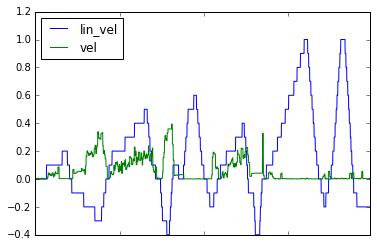
\includegraphics{motion_vs_cmd}
	\centering
	\caption{Commanded velocity (lin\_vel) as opposed to recorded motion (vel). Vel is always positive because it is measured in terms of euclidian distance moved by the center of the AprilTag between successive updates of the tag tracking. 
		Note that while the magnitude of the motion is proportional to the commanded motion, sometimes the robot did not move at all, and when it did move, the recorded velocity is quite noisy. Noise may be removed in software, mechanical failure cannot.} 
	\label{motor-speed-fig}
\end{figure}

This problem was highlighted by the use of inexpensive toys. 
It is desirable to have a swarm platform be able to run for extended periods, in order to acquire data for experiments. 
Toys, especially cheap ones, are designed for low cost and an MBTF more compatible with the attention span of children than that of researchers. 
The amount of effort devoted to locating and eliminating mechanical problems relative to the runtime of the system was not acceptable.

\subsection{Calibration} \label{section:Calibration}

Children's toys are prone to failure and inaccuracy.
In toys, particularly remote controlled toys, the user acts as a the feedback element of a control system, observing the behavior of the toy and changing their actions as a result. 
If an individual toy, for example, has a bias to turn to the left, the user will learn this and apply a correcting bias.
To extend this to a computerized system requires some form of calibration. 
These calibration steps, combined with appropriate control, such as PID loops, can account for systemic inaccuracies. 
However, the use of toys also introduces some failures which are not consistent or linear. 
For example, the tanks used in some instances of the TinyRobo platform use motors with high speed, but relatively low torque. 
As a result, dirt in the drivetrain near the motor can cause the motor to become difficult to start, but can be removed by the user, or by operation once the motor does start. 
Calibration when the dirt is present means the robot will start very abruptly when the dirt is removed, while calibration when the dirt is absent means the robot may not start if dirt gets into it later. 
It is worth noting, in light of this example, that GritsBots, Kilobots, and mROBerTO all use nearly-sealed drivetrains, either direct motor drive of the wheels or sealed vibration motors \citep{rubenstein2014kilobot, Kim2016mROBerTOAM, pickem2015gritsbot}. 

An early intent of the author was to have the system learn the control law for each robot through observation of the relationship between the commanded motion of the robot and the resulting motion. 
Due to the overarching concern with human control of a swarm, such online calibration was decided to be out of scope for this work. 
However, a computer-vision-guided calibration technique was used in the mROBerTO swarm robots to compensate for manufacturing differences between robots \citep{Kim2016mROBerTOAM}. 

This approach results in learning bad controls if the system observes the robot during a temporary failure. 
In a system with minimal failures, this problem can be minimized, but as discussed earlier, inexpensive children's toys are not such a system. 

GRITSBots have a calibration step, but the calibration is automated, and is only performed once for each robot, after which it is assumed that the calibration variables are constant.
Calibration can be automated in a homogenous platform with reasonably reliable hardware. 
Non-homogenous platforms require different calibration for different platforms, which reduces the benefit of automation. 
Further, requiring calibration works against transitioning to a new platform by adding an additional hurdle in the form of developing a new calibration method.

The lack of an automated calibration and control method drove the TinyRobo swarm to use more differential drive vehicles, as they struck a balance between the fully holonomic drive used in the SpiderBots, which is expensive but easy to control, and the Ackerman drive used in inexpensive RC cars, which is less expensive, but has more complex control math \citep{lairdspider}.
It also increases the difficulty of using a heterogenous system, and so operates against the advantages of heterogeneity as discussed in section \ref{section:Why_Heterogeneity_}

%\subsection{April Tag Latency} \label{section:April_Tag_Latency}
%
%April tags have very solid position and orientation tracking, but are computationally intensive to detect and localize in typical webcam images. 
%More tags leads to longer computation time, increasing the latency of the robot control loop. 
%Parallelizing the implementation of the AprilTag library could improve it significantly, but is out of scope for this work. 
%
%One version of the GRITSBots used AprilTags and a standard web cam, resulting in position updates at approximately 10Hz. 
%This update rate is consistent with that observed by the author using the ROS implementation of AprilTags. 
%Decreasing the size of the image in which the tags are detected speeds it up, at the cost of requiring larger tags in order to have them legible in the lower-resolution image. 
%The update rate places an upper bound on the ability of the system to respond to the motion of the robots. 
%To decrease the latency of this sensing, the GRITSBots team considered moving to color blob tags, which can be detected by the onboard vision processor of a Pixy CMUCam5 at up to 50Hz \citep{PickemGrits2014}. 


\subsection{Drive Testing} \label{section:Drive_Testing}

In order to characterize the behavior of the various toy hardware that the TinyRobo platform could be used on, seven TinyRobos were commanded by a program which instructed them to move forwards until the AprilTag tracking determined that they had moved a fixed distance, stop, and move again, in a loop. This program was run until the robot failed to move or ran into the walls of the robot arena.

Each robot was run 5 times, starting from the same location each time. The robot was power-cycled between runs. Each run was recorded using rosbag, and the data from the recordings were used to generate visualizations of the robot's commanded trajectory from the motion of the center of the robot's AprilTag.

The robots consisted of three toy tanks from the same manufacturer, a differential-drive Hexbug-brand robot, a differential-drive toy car with large wheels, a hexapod bug-like walker, and an Ackerman-drive toy car. 
The bug-like walker and the Ackerman-drive car both have different turning kinematics from the differential drive tanks, but this test only consists of forward drive.
It would have been preferable to have the test include turning, but control of the yaw rotation of a robot via feedback from the AprilTag system was found to be problematic. 
As the number of pixels that an AprilTag takes up on a camera image decreases, the accuracy of the subpixel estimation used to localize the corners of the tag decreases. 
Each estimation of the tag location from the ROS AprilTag detection node can then differ from previous estimations, and so even when the robot remains still, there is some noise in its detected position. 

The effect of the noise in subpixel position on the perceived rotation of the tags is larger than its effect on the perceived rotation of the tags, since rotation around the center of the tag does not change the position of its center at all. 
As a consequence, the tags could be detected to be in lateral motion by comparing the displacement of the center of the tag and checking that it was greater than the expected noise, but detection of rotational motion and velocity calculation was sometimes swamped by noise. 

The noise was also determined to be unevenly distributed over the robot arena. Because the arena is wide, a 140$^{\circ}$ wide-angle lens is used to ensure that the entire arena is visible. 
ROS provides tools for removing the distortion inherent in the use of a wide-angle lens, but at the cost of decreased effective resolution at the edges of the image. 
This decrease in resolution results in reduction of subpixel location accuracy, and so increased noise in localization of the tag at the edges of the arena closest to the edges of the camera image. 

Because the desired figure-8 motion could not be performed with the rotational localization noise present in the system, the robots were instead commanded to move forward 0.25m, stop, and repeat that sequence of actions until the program was stopped. 
The program was stopped if the robot was about to run into the wall of the arena, or had entered a state in which it could not move forward anymore. 
Acceleration during the movement phases was managed by increasing the commanded velocity of the robot until the AprilTag tracking detected that the robot had begun moving. 
Once the robot began moving, it was not commanded to change velocity until it had moved at least 0.25m.
In the following descriptions of the motions of the robots, the directions left and right are relative to the direction of travel of the robot. 

The Ackerman-steering toy car (page \pageref{img_traj}, image a) displayed very consistent mobility. In four out of its five runs, it crossed the arena without incident. 
In one run, it started and went a small distance, but then did not start again. 
However, the Ackerman-steering toy car has a gearbox that permits backdriving, so when commanded to stop, it coasts for a few centimeters. 
The toy tanks use a worm gear in their drivetrains, and so do not permit backdriving of the motors by the vehicle's inertia. 
Instead of coasting, they immediately stop when the motor is commanded to 0 velocity. 

The big wheel robot (page \pageref{img_traj}, image b) displayed an unfortunately small range of commanded velocities between those which caused it to begin moving, and those which caused it to flip over on its side.
In three of its five runs, the big wheel accelerated quickly and then flipped during the first motion period. 
In the remaining two runs, it did not move at all, possibly due to gears jamming. 

\begin{figure}
	\centering
	\begin{subfigure}[t]{0.3\textwidth}
		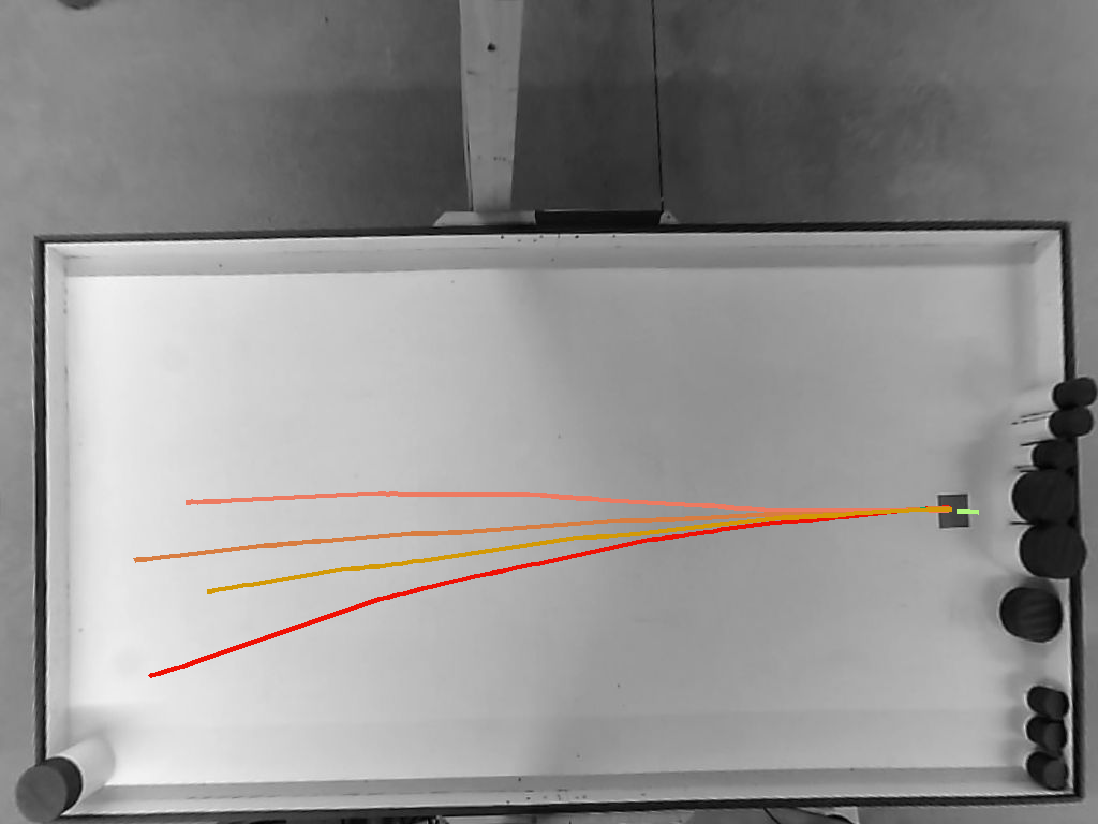
\includegraphics[width=\textwidth]{../hardwareX_paper/robot_17.png}
		\caption{Motion of toy car based robot}
	\end{subfigure}
	\begin{subfigure}[t]{0.3\textwidth}
		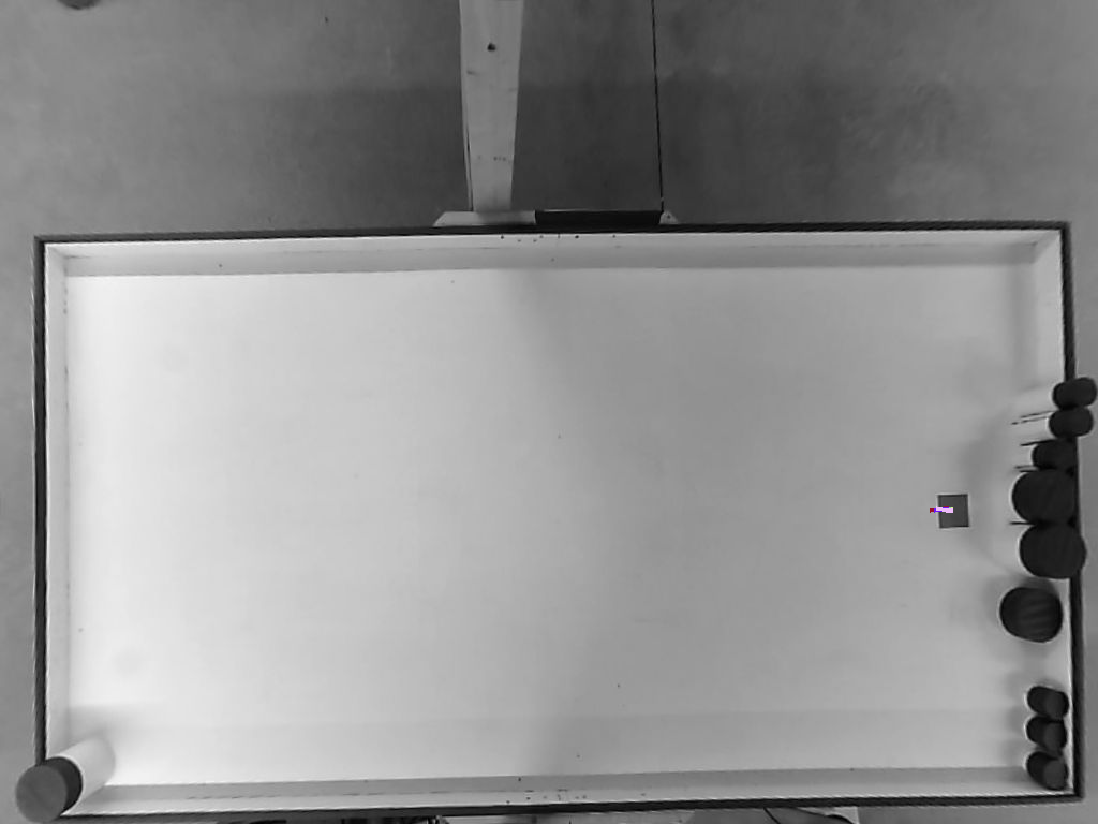
\includegraphics[width=\textwidth]{../hardwareX_paper/robot_1.png}
		\caption{Motion of big wheel robot}
	\end{subfigure}
	\begin{subfigure}[t]{0.3\textwidth}
		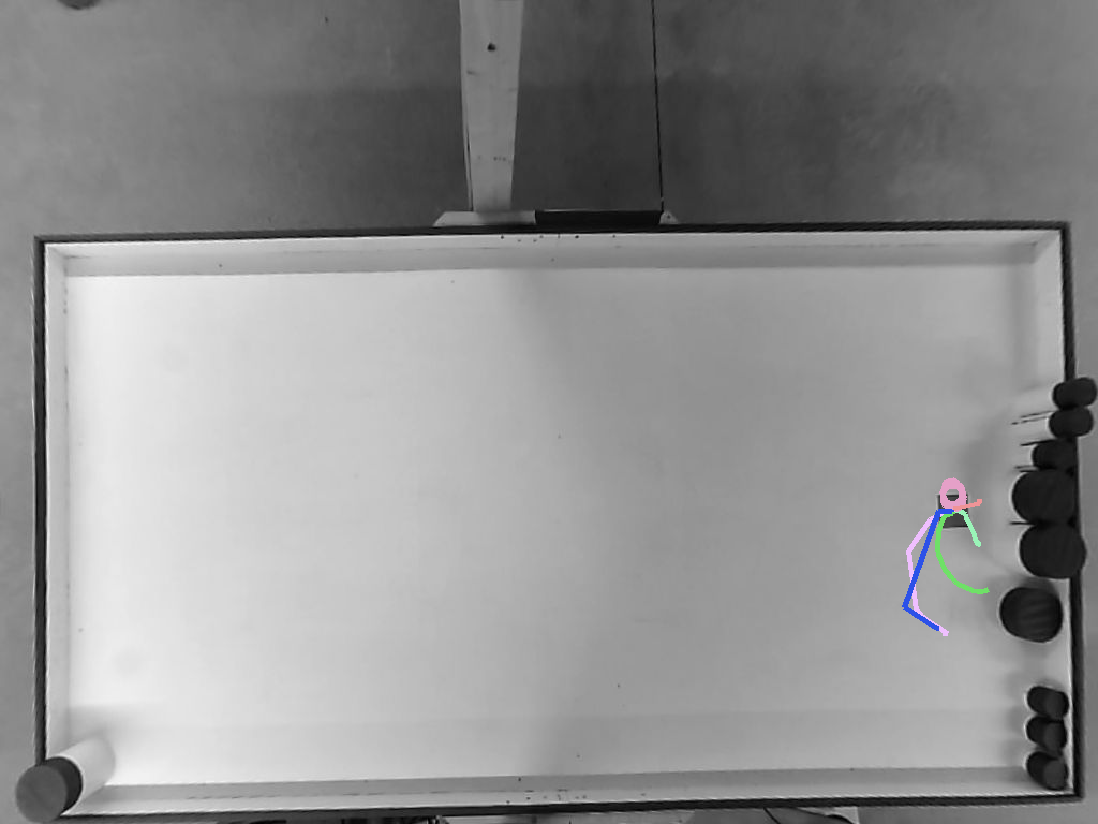
\includegraphics[width=\textwidth]{../hardwareX_paper/robot_6.png}
		\caption{Motion of 6-wheel bug}
	\end{subfigure}
	
	\begin{subfigure}[t]{0.3\textwidth}
		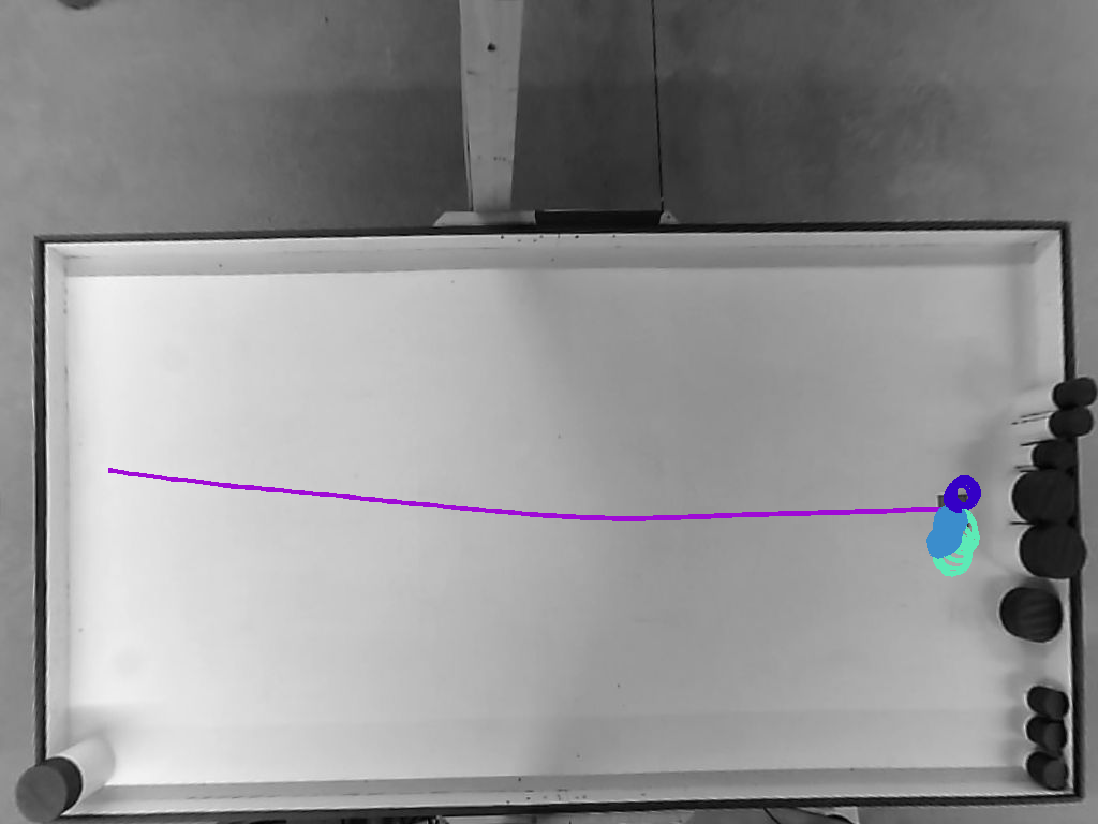
\includegraphics[width=\textwidth]{../hardwareX_paper/robot_0.png}
		\caption{Motion of green tank}
	\end{subfigure}
	\begin{subfigure}[t]{0.3\textwidth}
		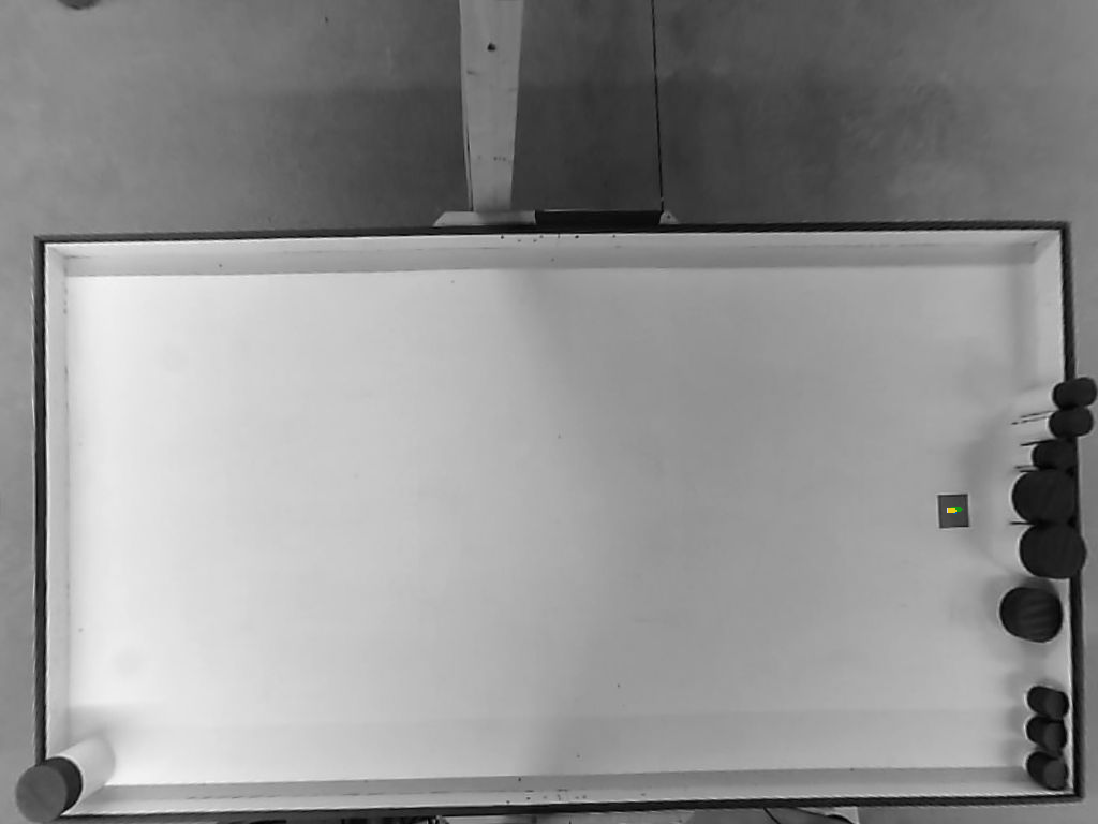
\includegraphics[width=\textwidth]{../hardwareX_paper/robot_8.png}
		\caption{Motion of blue tank \#8}
	\end{subfigure}
	\begin{subfigure}[t]{0.3\textwidth}
		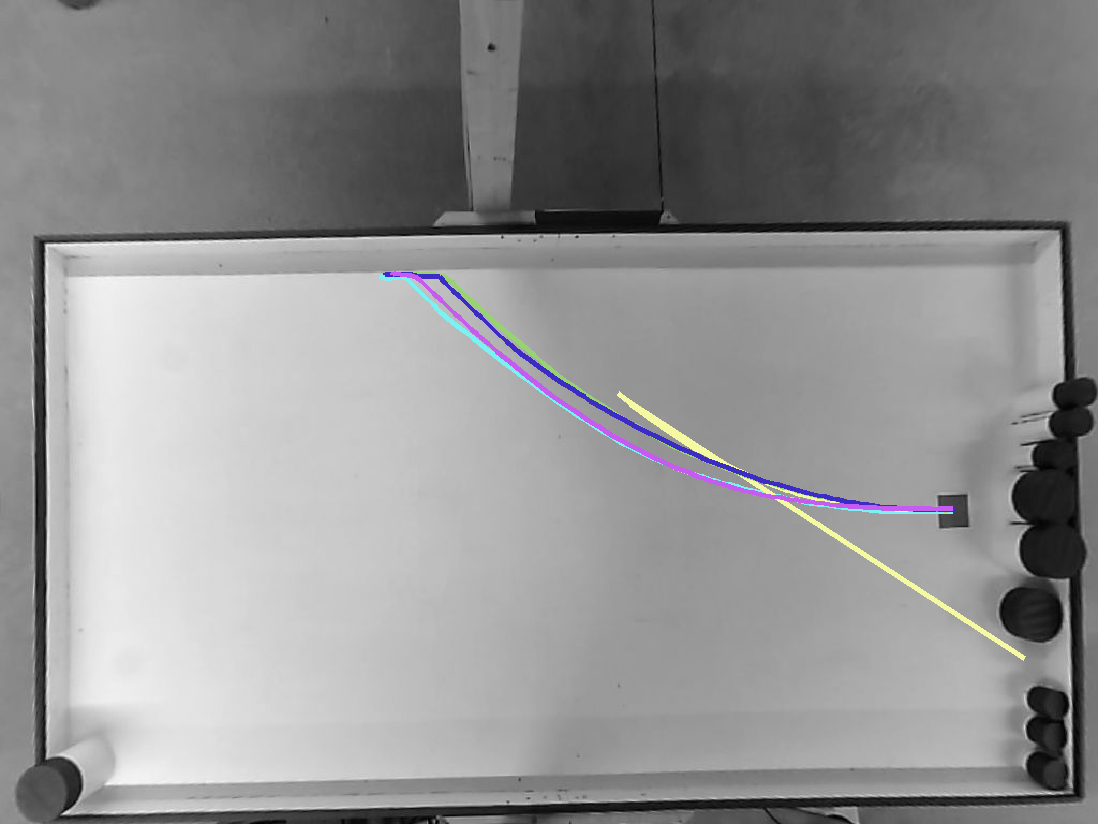
\includegraphics[width=\textwidth]{../hardwareX_paper/robot_18.png}
		\caption{Motion of blue tank \#18}
	\end{subfigure}
	
	\begin{subfigure}[t]{0.3\textwidth}
		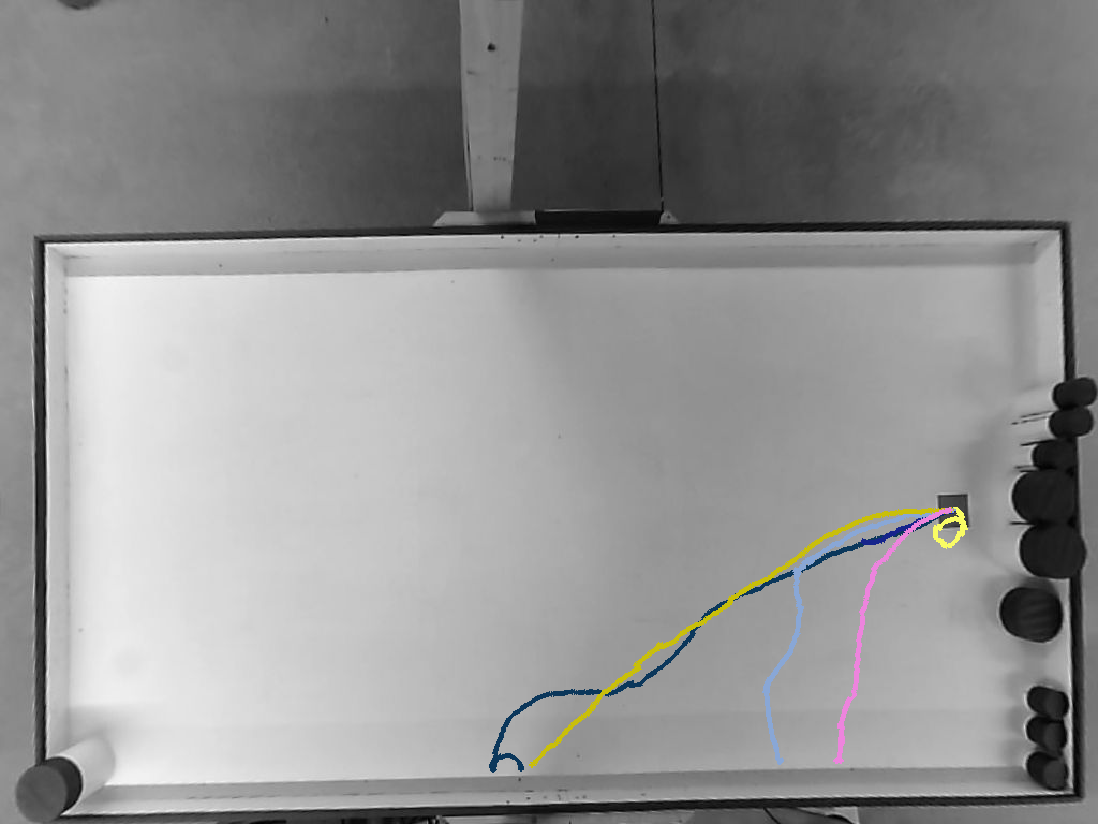
\includegraphics[width=\textwidth]{../hardwareX_paper/robot_5.png}
		\caption{Motion of bug robot}
	\end{subfigure}
	\label{img_traj}	
\end{figure}

The Hexbug-branded 6-wheeled bug (page \pageref{img_traj}, image c) displayed an asymmetry in its motor drive speeds. 
For three of its five runs, both motors ran, and the wheels on both sides rotated, but the right side was driven more quickly, and so the robot made a wide arc to the right and hit the wall of the arena behind the starting location. 
In one run, one side did not begin moving at all, causing the robot to rotate rapidly around that side. 
In another run, the robot twitched briefly, remained still, and then accelerated backwards quickly. 
This was likely caused by the gradual incrementing of the forward velocity eventually causing an integer overflow, resulting in a large forward velocity command being interpreted as a large negative velocity.

The green tank, carrying the number 0 AprilTag (page \pageref{img_traj}, image d), experienced problems with one side of its drive train in three of its five runs.
One tread drive did not move, while the other did, resulting in tight turns to the left in two runs, and to the right in one run. In one of the two remaining runs, the green tank did not move at all. In the second, the tank alternated movement and stopped periods until it reached the other side of the arena, which constituted success on this test. 

There are two blue tanks, carrying AprilTags numbered 8 and 18. 
Tank number 8 (page \pageref{img_traj}, image e) moved slightly on four of its 5 runs, and did not move on one of them. 
At no point did it move the full 0.25m. 
Tank number 18 (page \pageref{img_traj}, image f) moved much more consistently, but displayed an arc to the right in four of its 5 runs. 
In one run, the tank failed to restart after one of the stop phases, and eventually accelerated quickly in reverse. 
As with the 6-wheeled bug, this was likely the failure of the robot to move leading to a long enough delay that incrementing the commanded acceleration resulted in an integer overflow. 

The single-motor Hexbug-branded blue bug (page \pageref{img_traj}, image g) moved consistently, but with a heavy bias towards turning to the left. 
In every run, it started and stopped, but the curvature of the path to the left caused it to run into the left side of the arena. 
During one run, it fell over while moving, due to the somewhat ``bouncy'' nature of the toy's gait.

Some of these problems, such as the coasting of the Ackerman-steering car and the biases towards the left or right of some of the robots when commanded to move straight, can be overcome by software. 
For example, assuming the tags could be used to accurately measure the rotation of the robots, error between the detected rotational velocity and perceived rotational velocity could be accounted for in subsequent motion commands. 
The Ackerman-steering car drift could be reduced by sending a ``brake'' command to the motor driver IC to activate its back-EMF braking mode, rather than simply stopping by reducing the power output to zero. 
However, some of the problems are more difficult to alleviate. 
The tendency of the big wheel robot to flip over could be mitigated by very gradually increasing its speed, at the cost of reducing its control responsiveness, or by increasing the frequency of the feedback loop that checks its speed. 
Perhaps the blue bug would not fall over if its height were reduced, or the battery were placed lower on the body of the robot.
However, these mechanical problems could be more easily avoided by simply not using toys that have them. 

\subsection{3D Printed Robots}

Because the toys were demonstrated to be unreliable as motion platforms, a new design for the motion platform was developed using a 3D printer. 

The 3D printer used is the Monoprice Maker Select Mini (MPMSM), which costs approximately \$200 (US) at the time of this writing.
The MPMSM has a 120mm$^3$ build volume, and can print two robot chassis at the same time, as well as wheels for them. 
For this version of the TinyRobos, the motor selected was a commercially available miniature gearmotor. 
The gearmotor was selected because it was cheap, easily available from Amazon.com, and used the same voltage that the TinyRobo drive boards used. 
The motor has a planetary gearbox, and a plastic output shaft. 
Wheels were designed to be 3D printed along with the robot, and glued to the output shaft of the motor. 
3D printing provides the flexibility to change the motor mounts of the robot to accommodate various motors.

Because the 3D printed robots all used the same motors, there was no need to have them use an adaptive velocity control for drive testing as in the drive test for the toys. 
Instead, they could be commanded to move at a fixed velocity, and observed from the camera. 
However, the low output speed of the geared motors meant that the thresholds for detecting that the robot had stopped and started had to be changed. 
Once the program was adjusted so that it could detect the robot's motion or lack thereof correctly, the robots were commanded to move 0.25m, stop, move 0.25m and so forth until they ran into a wall of the arena. 
Once the robot hit a wall, it was reset and run again for 5 attempts. 
Each 3D printed robot was tagged with an April tag, numbered 2, 3, and 5. 

Robot 2 missed the first stop command on two of its runs, but worked normally for subsequent stop commands. 
It stopped and started regularly on the other three runs.
Robot 2 made a long arcing path to the left, indicating that one motor was running slightly faster than the other, or acquiring more traction.
This sort of error can be compensated for by feedback, assuming the robot can detect its own trajectory. 

Robot 3 missed all the stops on its first run and the first stop on its second run.
On its last three runs, it started and stopped as expected. 
Rather than arcing left as with robot 2, robot 3 arced to the right. 

Robot 5 also had an arc to the right. For its first run, it missed the last stop, but otherwise functioned correctly. 
On its second run, robot 5 started and stopped correctly, but hit something on the floor of the arena that caused it to turn more sharply right. 
On its third run, the system incorrectly detected that robot 5 had started after coming to a stop, and so began waiting for it to move 0.25m. 
The robot was not actually moving, so this condition would not have resolved. 
For run four, robot 5 stopped during its first move and did not restart.
The cause of this error is unknown, but it is possible that it was erroneously detected as having started before it did, and so was not sent motion commands to start. 
On the last run, robot 5 started and stopped as commanded until it was nearly at the wall, and then one wheel got stuck on a bit of wood on the arena floor, causing the robot to spin around that wheel. 

Overall, the 3D printed robots were more reliable than the majority of the toy bases, in terms of runs completed. 
However, a direct comparison cannot be easily made due to the changes that had to be made to accommodate the new bases. 
The use of a fixed velocity command for the forward motion is particularly problematic, as the gear ratio on the 3D printed robot motors is much higher than the gear ratio on most of the toys. 
As a result, a command that moves the 3D printed robots at 3-4cm/sec will set the toy tank bases moving too quickly for the camera to track them. 
The detection of robot motion also had problems due to the noise in the April tag detection and the low speed of the robots. 
Given more accurate tracking, the 3D printed robots could be expected to have fewer false starts and erroneously-detected stops. 

The 3D printed components of the robots do not add significantly to the cost of the robots. 
Material for 3D printers is generally sold in spools containing 1kg of filament for \$15-35, although some types of material are much more expensive, depending on the qualities of the material.
The robots described were printed in Hatchbox brand polylactic acid (PLA) filament, which costs \$20/kilogram. 
The resulting prints are \todo{get number out of cura}, and so contain \todo{how much?} worth of material. 

The motors used were listed on Amazon as "NW 3pcs 3V Micro Planetary Reducer Motor High Torque DC Motor DIY Robot Gearbox Motor". 
Unfortunately, these particular motors are from an unknown supplier, and as such, may become unavailable. 
However, a number of sellers are offering the same motors, or motors of similar size that could be used as replacements if the 3D print design were altered. 
The motors cost \$9.69 for a package of three, so \$3.23 each or \$6.46 for the pair needed for a robot. 
Given that the toys being used as mobility platforms cost \$8-20, depending on the volume purchased, even purchasing these motors at retail cost was a savings over using toys. 

\subsection{Guidelines For Future Swarm Developers}
The origin of the TinyRobo hardware platform was a hobbyist project, intended to combine the diminishing cost and increasing power of Internet of Things (IoT) networking modules with the ready availability of toys to create a system that lowers the barrier to development of multi-robot systems.
While it did not fully achieve this goal, there are a number of lessons that will be relevant to future developers of multi-robot research platforms. 

The drivetrain of the system is of paramount importance. 
Sensors and networking can be virtualized, as in TinyRobo and GRITSBots, but no amount of clever programming will compensate for balky motion. 
The use of direct drive, as in GRITSBots or mROBerTO, is encouraged because the resulting drive train will be sealed against foreign matter. 
Further, the use of stepper motors in GRITSBots provides some degree of precision in motion control by directing the motor in steps of known resolution, rather than commanding a particular speed. 
If the system requires additional torque, sealed micro gearmotors can provide increased torque (although with reduction in speed), and will be more reliable than adopting a drivetrain from a toy. 

The chassis of the robot can be constructed from the same printed circuit board (PCB) that the electronics are supported on. 
Over the scales of forces present in tabletop swarms, PCB can be considered completely rigid, and electronics solder provides sufficient mechanical strength for motor mounts. 
The use of custom mechanical assemblies in e.g. Jasmine micro robots adds complexity to the build process. 
Where possible, small robots should be designed to use the PCB instead. 
Using children's toys in TinyRobo was intended to avoid the use of such custom parts, but brought with it additional problems that were outside of the scope of the work to solve, and could have been avoided with a simpler drivetrain. 

Parts count for small robots should be minimized.
TinyRobo was developed around the ESP-8266 WiFi module because the module includes both a powerful microprocessor and wireless communication. 
Multi-use devices like the ESP-8266 are becoming cheaper and more competent quickly.
The processor in mROBerTO is both a 32-bit ARM processor, a low-power Bluetooth transceiver, and an ANT Wireless tranceiver. 
The VL6180X IC combines an ambient light sensor and a laser-based time-of-flight range sensor in a package measuring approximately 5x8x1mm. 
Reducing parts count reduces cost and speeds assembly. 

Swarm robots should have autonomous charging, and have each robot be able to monitor its own battery level. 
Any operation that requires user intervention with each individual robot will not scale well as the swarm size increases. 
In the case of the Kilobots, the swarm as a whole can be charged in parallel, rather than requiring the individual robots to be connected with a charger. 
For the GRITSBbots, pins on the front of each robot allows the robot to connect to a charging station by itself, rather than requiring a human to connect it. 
The TinyRobo platform could be trivially altered to provide GRITSBots-style self-charging, but does not at present have a method to detect a low battery condition, aside from monitoring the motor drivers for an undervoltage signal. 
The alternative to this, leaving out self-charging and battery monitoring, results in increased effort by humans to keep the batteries charged and failures due to discharged batteries that are not immediately obvious to the control software. 
At a more general level, hardware health monitoring is required for systems that intend to detect their own failed components and work around them, which increases robustness in a swarm system. 

The latency and accuracy problems with AprilTags could be mitigated in a number of ways. 
First, the resolution of the camera can be increased while keeping the tags the same size and the camera the same distance away. 

This solution ends up requiring more computational power as the image size increases, in order to keep the tag detection framerate high enough to be useful for realtime control. 
AprilTags have very solid position and orientation tracking, but are computationally intensive to detect and localize in typical webcam images. 
More tags leads to longer computation time, increasing the latency of the robot control loop. 
Parallelizing the implementation of the AprilTag library could improve it significantly, but is out of scope for this work. 

One version of the GRITSBots used AprilTags and a standard web cam, resulting in position updates at approximately 10Hz. 
This update rate is consistent with that observed by the author using the ROS implementation of AprilTags. 
Decreasing the size of the image in which the tags are detected speeds it up, at the cost of requiring larger tags in order to have them legible in the lower-resolution image. 
The update rate places an upper bound on the ability of the system to respond to the motion of the robots. 
To decrease the latency of this sensing, the GRITSBots team considered moving to color blob tags, which can be detected by the onboard vision processor of a Pixy CMUCam5 at up to 50Hz \cite{PickemGrits2014}. 
MROBerTO also used color tracking, with a single RGB LED on top of each robot to identify it, and a green LED on the front of each robot to indicate its orientation. 
Kilobot robots also include an RGB LED, which may be set to any color by the software of the Kilobot. 
These LEDs can also provide swarm feedback in a manner similar to the LEDs in McLurkin's Swarmish interface \cite{mclurkin2006speaking}.

Second, the tag size could be increased, either by moving the tags closer to the camera and increasing their visual size, or by actually making the tags larger. 
Moving the camera closer reduces the useful area of the robot arena, and making the tags larger increases the size and weight of the robots, potentially overbalancing some of the less nimble robots. 
As was observed in the robot drive tests, the bug and big wheel bases were already prone to tipping over. 


%\section{Swarm Simulation} \label{section:Swarm_Simulation}
%
%Because the sensors in the TinyRobo system are simulated, it may appear that the development of the UI and translation components could have been served as well by a simulated swarm as by a real one. 
%This is not the case. 
%In 1992, Rodney Brooks pointed out that ``there is a vast difference (which is not appreciated by people who have not used real robots) between simulated robots and physical robots and their dynamics of interaction with the environment'' \citep{brooks1992artificial}. 
%The gap between real-world sensing and actuation and their simulated counterparts means that developers working solely in simulation are tempted to either invest effort in solving problems that do not occur in the real world, or fail to solve problems that do arise in the real world but are left out of simulation. 
%One of Brooks' examples, the directional nap of carpet having an effect on robot odometry that varied with direction of travel, is still not handled by modern physics simulators. 
%Even if it were handled, the attempt would over-complicate simulation configurations due to the variety of types of carpet available. 
%
%Modern simulators have vastly more powerful computers behind them than they did in 1992, and the development of video games with realistic physics models has contributed greatly to the variety of physics models available in modern robot simulators. 
%As of 2015, however, Brooks' point still holds, and the dynamics of robots interaction with the environment are still not perfectly simulated \citep{erez2015simulation}.
%Generally, aspects of physics are elided or approximated from gaming physics engines, in favor of rapid simulation which is visually plausible. 
%In particular, contact dynamics simulations are NP-hard, and so are approximated in the interests of speed. 
%The PhysiX and Havoc physics engines also do not implement Coriolis forces at all.
%These sorts of omissions are mostly harmless, but evolutionary techniques for developing controllers for robots or simulated creatures can exploit them to develop control schemes that cannot work under real physics \citep{Brooks2000}. 
%
%In the real world, sensors are also uncertain. 
%Simulated sensors can provide a level of accuracy and certainty about that accuracy that is not available to real sensors operating with the sensor noise that affects real-world systems. 
%As the TinyRobo system simulates its laser and distance sensors, it may appear that it falls into this trap of simulation, and provides sensors that are ``too good to be true''. 
%However, the TinyRobo sensors are physical sensors, they're just not the same physical sensors that they are presented as, in much the way that a sonar sensor is not a ruler, but rather measures time and sound and presents it as distance. 
%Similarly, the arena camera is not a robot-mounted laser scanner, but it is still a physical optical sensor being used to measure distance
%\todo{test noise of camera based fake laser vs real lasers, characterize difference between multiple sensor readings of same thing}
%Adding noise to simulated sensors can also move them more towards the sensors available on real robots, but as Brook's carpet nap example indicates, the type of noise may be more complex than a simple normal distribution about the ground truth value. 
%With evolutionary approaches, the system can even come to depend on the noise, and fail when it is given real sensors that are less noisy then their simulated counterparts \citep{jakobi1995noise} 
%%Tim Smithers, "On Why Better Robots Make it Harder"
%	The idea that the variation in real robot behavior will go away if the robots are "better" as a justification for simulation
%	Better-made components allowing hunting where worse ones provided damping (steam engine governor example)
%	Don't view robots as measuring with sensors and reasoning about results
%		Sensors act as filters whose output drives internal robot dynamics
%
%An Overview about Simulation and Emulation in Robotics
%Michael Reckhaus, Nico Hochgeschwender, Jan Paulus, Azamat Shakhimardanov and Gerhard K. Kraetzschmar
%	Simulation went out of fashion when people started getting real robots
%	Computers got better and games drive for realism pushed development
%	Proposes a lot of use cases and reasons to use simulation
%		Which are interestingly orthogonal to the reasons not to use it
%			One doesn't counter the other, it's just "here are the good parts, here are the bad parts"
%
%Simulation in robotics
%Leon Zlajpah
%	Overview of tools





% !TeX root = ams_thesis.tex
\chapter{User Gesture Collection}\label{chapter:user_experiment}
\thispagestyle{fancy}

Multitouch gestural interfaces, like those found on tablets and smartphones, offer the possibility of a very direct user experience, especially compared to the Windows, Icons, Mouse, Pointer (WIMP) interface design. 
Rather than, for example, using an arrow key to scroll in a document, the user can drag the document directly, as though they were sliding a  piece of paper on a table. 

This directness is a hallmark of what has come to be called Natural User Interfaces, or NUI. 
A natural user interface is one that allows the user to re-use existing skills and natural motions to interact directly with content \citep{blakeNUIWin}. 
In practice, this means that the elements of the interaction are actions such as pointing and other gestures, drawing with a pen, speech, gaze, and so forth, rather than computer-specific interface devices. 
By way of contrast, the command line interface is defined in terms of typing with some form of keyboard, and the graphic user interface is (in most cases), defined in terms of mouse actions. 

However, as the number of operations the user wishes to perform increases, the limitations of multitouch screens become more apparent. 
Screens are flat, and so only afford 2-dimensional gestures, such as dragging, poking, and tapping. 
Even if the screen depicts a 2-dimensional projection of a 3-dimensional world, operations that would make sense in the 3D world, such as grasping, have to be mapped to the 2-dimensional space of operations to be performed. 
Typically, the gestures used to perform the available operations are chosen by the interface developer, and the user is trained to perform them, possibly by a short tutorial program \citep{wobbrock2009user, vanacken2008ghosts, freeman2009shadowguides}. 

Unfortunately, the use of screens with interactions inspired by the affordances of physical objects leads to the user having to decide between ``natural'' skills and motions, which are used on physical objects, and the skills and actions used with screens: single-point dragging and clicking. 
Most users understand that they are looking at pictures of things on a screen, and so default to single-point interactions \citep{vanacken2008ghosts}.
Further, tangible UIs, a subset of UIs that include real, physical objects for the user to interact with, raise a set of possible interactions that the designer may not forsee, or that the system may not be able to support \citep{hornecker2012beyond}.
Attempting to leverage the affordances of a physical object by depicting it on a screen adds another gap, where, in addition to failing to account for all of the affordances of the physical object (e.g. hitting it with another object), the system also fails to account for the affordances of a picture of an object (e.g. shrinking or enlarging it, which a real object cannot easily do). 
Additionally, even if these affordances are handled, they may not have clear meanings. 
What does it mean to use a photograph to hit a text file?

The behavior of users interacting with an NUI device is not solely informed by their intuitions about the physical objects represented on the screen. 
Smartphones, tablets, and other multitouch user interface devices, as well as specific types of computer programs, such as CAD and realtime strategy game programs, also inform the user's expectations about interactions with new interfaces. 
Rather than claiming that the users are untrained, and the gestures are ``intuitive,'' it would be more accurate to claim that the users already have a form of training, from the devices that they use in their daily lives. 
This work attempts to discover the gestures that users would choose themselves, based on their own thinking about the interface and their own past experience with computer technology such as tablets, smartphones, and video games. 

User-defined gestures have advantages in memorability and user preference over gestures designed by the researcher or interface programmer \citep{nacenta2013memorability}. 
However, the study that indicated this preference was for gestures that each user explicitly defined for themselves, rather than a gesture set that was constructed by eliciting gestures from the users during task execution \citep{Micire:2009:ANG:1731903.1731912}. 
By exending the task-oriented gesture collection from single or small groups of robots to swarms, this work attempts to discover if the gestures that users select vary with the number of robots available.

%More specifically, it is hypothesized that there exists a swarm size beyond which users will transition from treating the swarm robots as individuals to interacting with the robots in small groups or as a single large group. 
%This transition point will be apparent because of a change in the gesture set that users choose to interact with the swarm. 
%Rather than issuing one command for each robot, the user will instead use commands that control the bulk of the robots as a cloud or flock, but may leave some robots unused. 
%For example, the user may switch from selecting robots as individuals to shaping the group as if sculpting, with pushing and pinching to ``carry'' groups around. 
%The user may also change how they indicate which robots are to be interacted with. 
%Rather than selecting each robot by clicking on it, the user might circle a group they want to use, or simply assume that the same command is issued to all robots by default. 
%The size of the swarm where changes in the user gestures occur will indicate the transition point between the user intending to interact with individual robots as opposed to interacting with the swarm as a whole. 
%
%Further, it is hypothesized that altering how the user interface displays the location of the robots in the swarm will affect the transition point.
%Once the ratio of the size of individual swarm members to the size of the area the swarm is in becomes sufficiently small, displaying the swarm members at the same scale as the map will result in the representation of the swarm members being too small to interact with. 
%Scaling the representation of the robots up, relative to the map, could make the robot representations overlap unrealistically and obscure the map. 
%Instead, we propose that for certain scales of swarms, it makes sense to represent the swarm as the area covered by the swarm, rather than the locations of the individual robots.
%This approach has been used successfully for navigation in three dimensions, by developing a controller that causes the individual UAVs to remain within a bounding prism, and allowing the user to control the shape and location of that prism, instead of the location of each individual UAV \citep{ayanian2014controlling}.
%
%More specifically, a display which obscures individual robots and displays a cloud or swarm boundary will cause the user to treat the swarm as a whole rather than individuals, which will be apparent because the user will use the same gestures that users select for controlling individual robots. 

\section{Experiment Setup} \label{section:Experiment_Setup}

The multitouch user interface device used in this experiment is a 3M M2265PW touchscreen. 
This screen can track up to 20 simultaneous points, but reports only points, rather than shapes or areas of contact. 
While the user interacted with the touch screen, their touches and the positions of their hands were recorded by the computer connected to the screen and by the video cameras. 
One video camera was placed high, looking down at the screen, to track where the user's hand position over the screen. 
The other video camera was placed in front of the screen at a low angle, in order to observe whether the user's hands were touching the screen, or moving above it. 
In addition to screen contacts and video, users were asked to think aloud about their actions.
A microphone placed near the screen was used to record everything that the user said. 

\begin{figure}
	\centering
	\includegraphics[width=\linewidth]{../setup.png}
	\caption{Experiment setup, showing, L to R, the survey computer, microphone, cameras and multitouch interface device, and an example robot.}
	\label{fig:experiment_setup}
\end{figure}

The software used to record all of this information is ROS, the Robot Operating System \citep{ROS_announcement_paper}. 
ROS was developed as a message-passing framework and hardware abstraction layer for robots. 
Software using ROS is implemented as ``nodes,'' which communicate by passing messages, generally in a publisher/subscriber pattern. 
The format of the messages is formally defined, and the generation of the code for generating messages and handling routing of messages is provided by ROS. 

It may seem unusual to use a framework intended for operating robots as a recording program for collecting experiment data, but ROS provides a utility called rosbag that records some or all of the messages emitted by ROS nodes in a ``bag'' file. 
In this case, the cameras, microphone, and UI application are all recorded by rosbag.
A ROS launch file starts multiple ROS nodes to record image data from the cameras, audio from the microphone, and touch events and screen updates from the UI.
ROS also provides tools for manipulating bag files, and playing them back. 
All of the data in the file is timestamped, so it plays back with the audio, video, and UI interactions all accurately synchronized. 
Because all of the data is treated as standard ROS message types, it is relatively easy to write custom processors for the recorded data.
For example, a node was written that accepts the replayed UI screen changes and touch events, and renders them as a stream of ROS image messages showing the contact points overlaid on the UI screen. 
Ultimately, the entire data stream was rendered to video, as the rosbag playback does not support rewinding the playback, and being able to re-view a section conveniently was useful for coding. 

Users were seated in front of the interface and read a script describing the system and the experiment. The user interface displayed alternating slides of instructions to the user, such as ``Move the robots to area A", and interface screens for them to interact with. 
The interface did not visibly respond to user contact or move the robots depicted on it.
In this regard, it more closely resembles the paper prototypes of the User-Centered Design process than a fully functional interface \citep{ehn1992cardboard}.

Some users were initially confused by the interface not responding. 
It may be that running this experiment on a computer, rather than a paper prototype, contributed to the user expectation that the system could react.
Paper prototypes, obviously, do not change in response to the user performing an action, although the experimenter may show the user new sheets of paper depicting the next state of the interface. 
However, most users' experience with touch screens is that when they touch them, something visible happens nearly immediately. 
A system that does not visibly react, as in this experiment, is usually assumed to be broken, or waiting for further input.

For future work, it may be desirable to structure attempts to elicit user gestures as in Wobbrock \emph{et al.} \citep{wobbrock2009user}. 
The experiment described in this section showed the initial situation, and asked the users how they would make a specific change. 
Wobbrock \emph{et al.} showed the change occurring, and then asked the users what command they would issue to cause that result. 
Showing the response before asking for the gesture removes the expectation that the system will react. 

Unfortunately, showing the response of the system may also act as a cue to the user that suggests a specific solution for gesture selection. 
For example, if the system shows a square formation being formed by multiple robots moving directly to the closest point on the square to their starting location, the paths shown are multiple direct motions. 
If instead, the system shows the robots forming a chain that snakes around the perimeter of the square before coming to a stop, the path shown is forming the snake, and then traversing the perimeter. 
The motion in the first case may suggest that the user make individual gestures to position each robot, while the gesture suggested in the second case might be more like dragging a lasso around the group and then a line from the group around the perimeter of the box. 
Even for simple cases like moving to a target area, if the robots are shown moving along a path, it might discourage the user from using waypoints instead of dragging a path.


\subsection{Experiment Conditions} \label{section:Experiment_Conditions}

Each user was assigned to one of five conditions, varying by how many robots were in each condition. 
The conditions consisted of 1-2 robots, 10 robots, 100 robots, 1000 robots, or an unknown number of robots.
In the unknown number condition, the area the robots were present in was represented by a cloud. 
For each condition, the user was requested to perform a sequence of tasks. 
The exact number of tasks varied between conditions due to some tasks not making sense with the number of robots involved, as shown in Table \ref{tab:tasks_per_condition}. 

\begin{figure}
	\begin{subfigure}{\textwidth}
		\centering
		\fbox{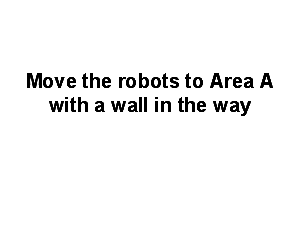
\includegraphics[width=0.4\textwidth]{../ui_experiment/slide_images/Swarm_Robot_Control_-_10_Robot_0004.png}}		
		\fbox{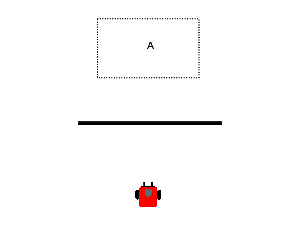
\includegraphics[width=0.4\textwidth]{../ui_experiment/slide_images/Swarm_Robot_Control_-_Single_Robot_0005.png}}
	\end{subfigure}
	\vspace{2mm}
	
	\begin{subfigure}{\textwidth}
		\centering
		\fbox{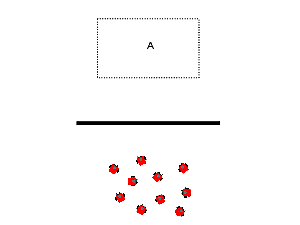
\includegraphics[width=0.4\textwidth]{../ui_experiment/slide_images/Swarm_Robot_Control_-_10_Robot_0005.png}}		
		\fbox{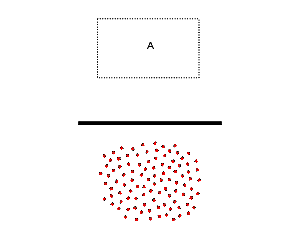
\includegraphics[width=0.4\textwidth]{../ui_experiment/slide_images/Swarm_Robot_Control_-_100_Robot_0005.png}}	
	\end{subfigure}
	\vspace{2mm}
	
	\begin{subfigure}{\textwidth}
		\centering
		\fbox{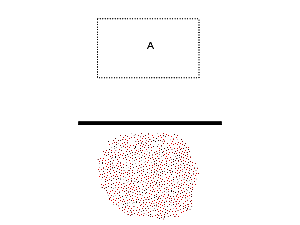
\includegraphics[width=0.4\textwidth]{../ui_experiment/slide_images/Swarm_Robot_Control_-_1000_Robot_0005.png}}		
		\fbox{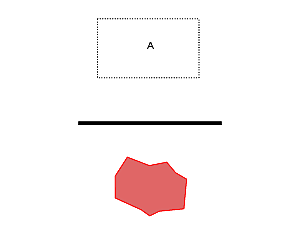
\includegraphics[width=0.4\textwidth]{../ui_experiment/slide_images/Swarm_Robot_Control_-_Unknown_Number_of_Robots_0007.png}}
	\end{subfigure}
	\caption{Instructional slide and situations for moving around the wall to area A, in each condition.}
	\label{fig:move_around_wall}
\end{figure}

\begin{table}
\begin{tabular}{l|l|l|l|l|l}
	& 1 & 10 & 100 & 1000 & Unknown \\
	Move to area A & x & x & x & x & x\\
	Move to area A with a wall & x & x & x & x & x \\
	Stop the robots & x & x & x & x & x\\
	Divide around an obstacle & & x & x & x & x \\
	Orange to B, red to A & x & x & x & x & x \\
	Orange to A, red to B & x & x & x & x & x \\
	Orange to A, red to B (mixed) & x & x & x & x & x \\
	Divide group & x & x & x & x & x \\
	Merge groups & & x & x & x & x \\
	Form a line & & x & x & x & x \\
	Form a square & & x & x & x & x \\
	Move the crate to area A & x & x & x & x & x \\
	Move the crate to area A (dispersed) & x & x & x & x & x\\
	Mark defective robot & x & x & x & x & \\
	Remove defective robot & x & x & x & x &  \\
	Patrol the screen border & x & x & x & x & x \\
	Patrol area A & x & x & x & x & x \\
	Disperse over screen & x & x & x & x & x \\
\end{tabular}
\caption{User tasks per condition.}\label{tab:tasks_per_condition}
\end{table}

The individual robot case is lacking the tasks that do not make sense for a single robot. A single robot cannot, for example, divide around an obstacle or form a square. 
The ``Merge groups" task was left out of the single robot case because of the potential for confusion when referring to a single robot as a group. 

The unknown number of robots condition has the same tasks as the 10, 100, and 1000 robot cases, except for the ``Mark defective robot" and ``Remove defective robot" task. 
Without UI elements that represent individual robots, the user cannot take any actions that refer to a specific robot. 



\subsection{Participant Demographics} \label{section:Participant_Demographics}

Participants were recruited through fliers distributed on campus and in the surrounding city. 
The recruitment process and experiment were approved by the UMass Lowell institutional review board.
The experiment had 50 participants, 10 in each condition. 28 of the participants were male, 22 were female. The average age of participants was 22.1 years, with a standard deviation of 3.16. 

These demographics are representative of the location that the study was performed, the campus of an American college. 
It has been suggested that research in psychology focuses too much on a population that is WEIRD (Western, Educated, Industrialized, Rich, and Democratic), and that the results of such studies may not generalize beyond that population \citep{arnett2008neglected}.
However, for the purposes of this study, particularly assessing the influence of smartphone use on expectations of user interface gestures, it is useful to have a population with significant experience using smartphones, which are a product of both rich and industrialized societies. 
It is not proposed that the results of this work generalize to humanity as a whole.  

\section{Analysis} \label{section:Analysis}

User gestures were coded using a methodology adopted from the social sciences, Grounded Theory \citep{glaser2017discovery}.
Grounded Theory is an iterative process, where the data are first coded at a very fine-grained level, and then the resulting coded elements are compared to each other to try to determine their qualities, similarities, and differences. 
Codes can be consolidated or divided until repeated passes of coding and comparison no longer alter the emerging structure of the coding scheme. 
During each iteration of coding and comparison, the coder makes memos as well, describing the links they see between related coded elements and higher-level abstractions that relate the elements. 
These memos are eventually written up as a social scientific theory that is believed to be grounded in the data because it arises from the coding process. 

\subsection{Initial coding pass} \label{section:Initial_coding_pass}

The inital pass used open coding, where the ``codes'' were essentially free-form text entry. 
Rough counts of the open codes for the first 10 participants indicated that ten of the codes covered 81\% of the 580 total coded events. 
The ten most heavily used codes are, in order of occurrence: drag, tap, voice command, box select, 2 finger drag, double-tap, lasso, tap and hold, 2 handed drag, reverse pinch, and parallel hands. 
This coding pass indicated that a majority of the user actions could be coded as some form of drag, some form of tap, box or lasso selection, pinch, and parallel hands. 

The most common code was ``drag'', which accounts for 37.58\% of the rough coding, or 42.07\% if all forms of drag in the top ten codes are considered. ``Drag'' is when the user places one finger down, moves it to another location, and raises it again. Two finger drag is the same, only with two fingers on the same hand placed on the screen rather than one. Two-handed drag is single-finger drag, but executed with both hands at the same time. 

The second most common code was ``tap'', with 20.34\% of the rough coding, or 25.34\% if tap, double-tap, and tap and hold are all considered. Tap is when the user places a finger down and then very quickly raises it again. Double-tap is two taps in the same location in quick succession. Tap and hold is when the user places their finger on the screen and leaves it in one place for more than a second before raising it. 

Box select consists of a diagonal (relative to the screen edges) drag gesture over the robots or another object on screen, with the intent to select everything within the box whose diagonal is represented by the drag. 
Lasso select is a drag that ends near where it began, forming a loop, with the intent to select everything inside the loop. 

Pinch and reverse pinch are essentially two-hand drag or two-fingered drag but with the hands or fingers moving towards (pinch) or away (reverse pinch) from each other.
This gesture is common for zooming in multitouch user interfaces on smartphones. 

Voice command was used to code when a user spoke a command out loud, rather than using gestures. The high incidence of voice commands (7.07\% of all codes) in the first ten users can be attributed to a single user who issued commands almost exclusively through voice. 
The final gesture, ``parallel hands'' is placement of the hands, palms facing each other, over some area of the screen. This gesture was used many times by the same user who issued voice commands, to indicate where the robots should form a line. Because parallel hands only accounted for 0.69\% of the gestures, it was left out of the development of the coding application for the second stage of coding. 

\subsection{Second Coding Pass} \label{section:Second_Coding_Pass}

To facilitate coding in the second pass, an application was developed to record codes. 
The application has coding functions for the six most common gestures: drag, tap, voice command, box select, lasso select, and pinch. 
It also includes coding functions for user interface elements described by the user, such as buttons or menus, a function to code user gestures not covered by the six most common gestures, and a function for coders to enter free-form text memos. 

A second pass of coding of the first ten user recordings was performed by two coders. 
Because the coders were responsible for deciding which user actions to code, as well as how to code them, it is possible for one coder to miss a gesture that another coder codes, or to split a single gesture into two coded units instead of one. 
For example, one coder initially split spoken commands at conjunctions such as ``and", resulting in two units both coded as voice commands, while the other coder coded the entire sentence as a single unit. 
This leads to the possibility that for a single task, the coders will produce different length lists of coded units. 

Cohen's $\kappa$ is a measure of inter-coder reliability for categorical items, but it assumes that both coders are coding the same number of codable units \citep{cohen1960coefficient}. 
In order to calculate inter-coder reliability in the presence of potentially missing data, the  shorter of the two lists of codes for each task was padded with a code for ``no data". 
The codes were then aligned chronologically, with pairs consisting of an item from each list such that the total time error within the task was minimized.
As a result, the alignment process created pairs of a valid code and the ``no data" code for the codes in the longer list that did not have a good chronological match in the shorter list.
This was based on the assumption that the source of the error is one coder missing an event that did occur, rather than the other coder coding an event that did not occur. 

The initial pass of coding got poor inter-coder reliability, with the first 10 participants having an average Cohen's $\kappa$ of 0.422. % 0.357, 0.266, 0.398, 0.387, 0.643, 0.428, 0.407, 0.56, 0.273, and 0.502. 
Cohen's $\kappa$ of over 0.75 is excellent agreement, 0.4-0.75 is fair, and below 0.4 is poor, so the average $\kappa$ was barely above the cutoff for fair agreement \citep{Fleiss_stats_methods}. 

Analysis of the data, particularly with confusion matrices, showed several problems. 
The simplest was training error in the training of the coders.
One coder had not been instructed that the ``UI'' code existed, and so had coded user interface widgets as ``tap'' events.   
This was immediately apparent in the confusion matrix as a very high confusion between UI and tap events. 
The other main source of confusion was lasso and box selection actions being coded as drag events, and vice versa.
The actual action performed in a lasso is a drag, in that the user puts their finger down and drags it in a circle around something before lifting it again, but it is intended as a selection of the things inside the circle rather than e.g. drawing a circle shape. 

In order to reduce these errors, and ensure consistency in training the coders, the descriptions for each code were written up in discussion with the coder, so that questions about interpretations could be answered in advance and recorded. 
The codes were box selection, lasso selection, drag, tap, pinch, ui widgets, voice command, and other. 
The coding definitions, as presented to the coders, are documented in Appendix \ref{chapter:coding_defs}.
Another coder was trained with the code description document, and coded the first 5 participants. 
This coder obtained an average Cohen's $\kappa$ of 0.794 with one of the original coders.
These values indicate a very high level of agreement, so the remaining videos were coded by these two coders, using the description of the codes from the code description document.  

The resulting data set had 3,256 individual gestures coded. 
For analysis, drags that were used to draw something on the screen were separated from non-drawing drags. 
Taps were separated into single, double, and triple taps, plus tap and hold. 
Pinch was separated into pinch (where the contact points move towards each other) and reverse pinch (where the contact points move apart).
All of these divisions were based on modification flags recorded by the coders during the coding process.  
\begin{table}
	\centering
	\begin{tabular}{l r r}
		Gesture & Count & Percent\\
		\hline
		Drag & 1084 & 33.29 \\%24 \\
		Draw & 761 & 23.37 \\%22 \\
		Tap & 514 & 15.78 \\%62\\
		Other & 189 & 5.80 \\%47 \\
		Lasso & 184 & 5.65 \\%11 \\
		Box Select & 113 & 3.47 \\%05 \\
		UI & 112 & 3.43 \\%98\\
		Double tap & 95 & 2.91 \\%77 \\
		Hold & 66 & 2.02 \\%70\\
		Reverse Pinch & 49 & 1.50 \\%49 \\
		Voice & 44 & 1.35 \\%13\\
		Pinch & 26 & 0.79 \\%85 \\
		Triple Tap & 19 & 0.58 \\%35\\
	\end{tabular}
	\caption{Gestures used by experiment participants, by count and as a percentage of the total gestures used. This table includes example gestures in the counts, as defined in appendix \ref{chapter:coding_defs}.}
\end{table}

\section{Selection Gestures} \label{section:Selection_Gestures}
One area in which the gestures were expected to change between conditions is the use of selection gestures. 
The intuition behind this expectation is that for small numbers of robots, there is no need for a gesture that selects groups, as the user can interact directly with each robot. 
Similarly, in the case where no individual robots are displayed, the use of group selection gestures would be minimal, as the group is presented as a single cloud. 

Users performed selection of robots in groups by box select, lasso, and UI interactions.
These selections were counted by condition by counting lasso or box events that had a robot or robots as their targets. 
Single selections of robots were performed by tapping on the robot. 
Similarly to the count of group selections, tap events were counted where the object of the tap event was a robot or robots. 


\begin{table}
	\centering
	\begin{tabular}{l r r r r}
		Condition & Box Select & Lasso & Tap & Total (condition)\\
		\hline
		Unknown & 0 & 1 & 43 & 44 \\
		One & 0 & 3 & 78 & 81\\
		Ten & 26 & 105 & 140 & 271\\
		Hundred & 68 & 53 & 35 & 156\\
		Thousand & 18 & 16 & 22 & 56\\
		\hline
		TOTAL & 112 & 178 & 318 & 608\\
	\end{tabular}
	\caption{Per-condition total use of selections}
\end{table}


The ten robot case has the most selection gestures for either group or single selection. 
As was expected, the unknown number and single robot cases have very low counts of group selections. 
Interestingly, the thousand robot case also has relatively low group and single 
selection use, especially compared to the ten robot case. 

To determine if these differences were statistically significant, the count of each user's gestures per task were normalized by dividing by the total number of gestures that user used to perform the task. 
Normalizing in this manner converts raw gesture counts to a proportion of the total gestures used on that task, preventing more verbose users from dominating the analysis.

The tasks checked for statistically significant differences between conditions were those that all conditions had in common. 
These nine common tasks are `move crate', `divide by color (cross)', `divide by color', `move to a', `move to a (wall)', `patrol a', `patrol screen', `split', and `stop'. 
Across all the common tasks the proportions of each gesture were collected per gesture, resulting in, for each gesture, 5 lists, one for each condition. Each list consists of 90 entries, 10 users times 9 common tasks. Each list entry consists of the proportion of that gesture the user used to complete the task. ANOVAs were performed for each pair of conditions. 

For uses of tap as selection across the common tasks, the unknown number condition differs from the hundred (F=7.6964, p=0.0061) and thousand (F=5.5772, p=0.0193) robot conditions. 
The one robot condition differs from the ten (F=4.3299, p=0.0389), hundred (F=13.5889, p=0.0003), and thousand (F=10.4274, p=0.0015) robot conditions.
These differences are summarized in Table \ref{tab:tap_select_per_task_norm}.

\begin{table}
	\begin{tabular}{l|r r r r r}
		& unknown & one    & ten        & hundred     & thousand   \\ 
		\hline
		unknown & & 0.5622 & 0.1772 & \textbf{0.0006} & \textbf{0.0193} \\   
		one & & & \textbf{0.0389} & \textbf{0.0030} & \textbf{0.0015} \\
		ten & & & & 0.1089 & 0.2719   \\
		hundred & & & & & 0.5457   \\
		thousand & & & & &\\
	\end{tabular}
	\caption{P-values for the use of tap as select between conditions}
	\label{tab:tap_select_per_task_norm}
\end{table}

For uses of group selection across the common tasks, the unknown number condition differs from the ten (F=47.635915, p \textless 0.0001), hundred (F=60.435124, p \textless 0.0001) and thousand (F=10.2346959, p=0.0016) robot conditions. 
The one robot condition differs from the ten (F=47.6359, p \textless 0.0001), hundred (F=60.4351, p \textless 0.0001), and thousand (F=10.2347, p=0.0016) robot conditions.
The ten robot condition differs from the thousand robot condition (F=19.0110, p \textless 0.0001).
The hundred robot condition differs from the thousand robot condition (F=30.2373, p \textless 0.0001).
The identical F and p values for the one and unknown robot conditions and the various conditions that they differ from are because for the one and unknown robot conditions, no group selection gestures were used in the common tasks. 
These differences are summarized in Table \ref{tab:group_select_per_task_norm}.

\begin{table}
	\begin{tabular}{l|r r r r r }
		& unknown & one    & ten        & hundred     & thousand   \\ 
		\hline
		unknown & & * & \textbf{0.0000} & \textbf{0.0000} & \textbf{0.0016} \\   
		one & & & \textbf{0.0000} & \textbf{0.0000} & \textbf{0.0016} \\
		ten & & & & 0.1808 & \textbf{0.0000}   \\
		hundred & & & & & \textbf{0.0000}   \\
		thousand & & & & &\\
	\end{tabular}
	\caption{P-values for the use of group selections between conditions. The ANOVA between the unknown case and the single robot case was not computable, as no group selections were used for the unknown case or the single robot case for the common tasks.}
	\label{tab:group_select_per_task_norm}
\end{table}

\begin{table}
	\centering
	\begin{tabular}{l | r r }
		& common tasks & all tasks\\
		\hline
		unknown & 0 & 1\\
		one & 0 & 3\\
		ten & 55 & 107 \\
		hundred & 60 & 109\\
		thousand & 15 & 28\\
	\end{tabular}
	\caption{Counts of group selection gestures in the common tasks and all tasks.}
	\label{tab:group_raw_counts}
\end{table}

\begin{table}
	\centering
	\begin{tabular}{l | l l}
		& common tasks & all tasks\\
		\hline
		unknown & 15 & 29\\
		one & 38 & 53 \\
		ten & 45 & 108\\
		hundred & 4 & 29 \\
		thousand & 7 & 18\\
	\end{tabular}
	\caption{Counts of tap selection gestures in the common tasks and all tasks.}
	\label{tab:tap_raw_counts}
\end{table}

Examining the non-normalized counts of taps as selections and group selections across both the common tasks and all tasks indicates that heaviest use of tap selection is in the ten robot case. Heaviest use of group selection is in the hundred robot case, but the ten robot case only lags it by two uses. The second heaviest for group selection is the hundred robot case, while the second heaviest for tap selection is the single robot case. This seems to indicate that with single robots, users prefer tap selection, with one hundred robots they prefer group selection, but with ten robots, either selection method could be viewed as appropriate. 

It was surmised that users may have been performing multiple tap selections in a row to select robots in the ten robot case, but that a 10-robot tap selection would be condensed by the normalization into the same proportion of the overall gestures as a single-robot tap selection. 
To check if users were performing multiple taps in a row as selections, the lengths of sequences of tap actions were checked across all cases. 
As seen in Table \ref{tab:tap_seq_len}, while the ten robot case does have a much higher count of sequences of taps, the mean is higher than the other cases, and the standard deviation is much higher. 
On examining the data, there was exactly one case of a 10-tap sequence in the ten robot case.
While it is possible that a user in the ten-robot case might perform a selection by tapping each of the ten robots, it is not a common occurrence. 

\begin{table}
	\begin{tabular}{l | r r r}
		& Sequence Count & Mean Length & Standard Deviation \\ 
		\hline
		unknown & 28 & 1.0357 & 0.1856 \\
		one & 42 & 1.2619 & 0.5798\\
		ten & 72 & 1.5000 & 1.6499\\
		hundred & 23 & 1.2609 & 0.4391\\
		thousand & 17 & 1.0588 & 0.2353\\
	\end{tabular}
	\caption{Lengths of sequences of taps within conditions.}
	\label{tab:tap_seq_len}
\end{table}

% TRIPLE CHECK THIS BEFORE USING ANY OF IT
%For the box selection gesture, the unknown condition differs significantly ($\alpha$ = 0.05) from the ten (F=7.17386 p=0.00809), hundred (F=26.95175 P=0.00000), and thousand (F=4.57743 p=0.03376) robot conditions, but not from the single robot condition (F and p values could not be calculated due to disuse of box selection in these cases). 
%The use of box select in the one robot condition differs significantly from the ten (F=7.17386 p=0.00809), hundred (F=26.95175 p=0.00000), and thousand (F=4.57743 p=0.03376) robot conditions.
%The hundred robot condition differed from the ten (F=9.17884 P=0.00281) and thousand (F=13.81053 P=0.00027) robot cases. 
%
%
%
%For the lasso gesture, the unknown condition differs significantly from the ten (F=33.27742 P=0.00000), hundred (F=19.44664 P=0.00002), and thousand (F=5.86234 P=0.01647) robot cases. 
%The one robot condition differs significantly from the ten (F=33.27742 P=0.00000), hundred (F=19.44664 P=0.00002), and thousand (F=5.86234 P=0.01647) robot cases as well. \todo{Why are these differing by the same amount between unknown and one? The same proportions?}
%The thousand robot condition also differed from the ten (F=23.51414 P=0.00000) and hundred (F=11.76321 P=0.00075) robot conditions. 
%
%For the tap gesture, the unknown condition differs significantly from the one (F=5.07967 P=0.02543) and thousand (F=5.31693 P=0.02227) robot conditions. 
%The one robot condition differs from the ten (F=5.58672 P=0.01918), hundred (F=7.47952 P=0.00687), and thousand (F=21.15146 P=0.00001) robot conditions. 
%The thousand robot also differs from the hundred robot condition (F=4.08954 P=0.04465), although not as strongly as many of the others. 
%However, this analysis looks at all uses of tap, not just tap intended as select, as detected by the object of the tap being a robot.
%
%To determine if tap-as-select, rather than just any use of tap, maintained this relationship, the count of group selects (box or lasso with robots as the object) and single selects (taps with robots as the object), were collected, per user across all tasks that are common to all conditions. 
%These lists were averaged, to get the average use of group select or single select, for each task, averaged across the condition.\todo{This is raw counts, should maybe do this and then normalize to get proportions, rather than average.}
% 
%For tap-as-select, the hundred robot case differed from the unknown (F=5.61783, p=0.03068), one (F=9.13207, p=0.00810) , and ten (F=6.59643, p=0.02062) robot cases. The thousand robot case differed from the ten (F=5.64536, p=0.03033) and one (F=7.62757, p=0.013893) robot cases.
%
%For group select, the hundred robot case differed from the unknown (F=5.61783, p=0.03068), one (F=9.13207, p=0.0081) , and ten (F=6.59643, p=0.02062) robot cases. The thousand robot case differed from the ten (F=5.64536, p=0.03033) and one (F=7.62757, p=0.01389) robot cases.



%The gestures draw, pinch/reverse pinch, and double-/triple-tap did not display any statistically significant difference across conditions in the common tasks. 
%Pinch/reverse pinch were somewhat task-specific gestures, used across condition to divide/merge groups of robots in that task. 
%
%Draw is also somewhat task specific, mostly used in formations to draw the target shape. However, the formation tasks are not in the common task set, because a single robot cannot form a formation. 
%
%Were double and triple taps also specific to some task? This would be interesting to check, because it seems to indicate a division of gestures into gestures that were related to a task, and gestures that were related to a condition. 
%
%Graphing \todo{put the graphs in here} average per-user proportion of gestures per task indicates that pinch or reverse pinch were highest in divide color 1, patrol a, patrol screen, and split. Split had by far the most reverse-pinch gestures. 
%
%Draw peaked for split and stop. For split, this was caused by users drawing a dividing line between the split groups. For stop, it was caused by users drawing a line in front of the robots to indicate a virtual barrier. If the formation tasks were in the common task set, they would also likely have large numbers of draw gestures. 
%
%Doubletap peaked in the stop case as well, but triple taps occured at a very low level in crate, divide color 1, and move a, and at a slightly higher level in patrol screen and split. In general, tripletap may not have enough samples to make a comparison meaningful. It was only used 19 times total, and is the least common gesture. 

\section{Multi-hand Gestures}

Multi-hand gestures fall into two different groups. \
The first group is gestures where each hand is performing part of a single gesture.
Generally, these were pinches and reverse pinches with one finger on each hand. 
%[PUT COUNT HERE] users also performed two-handed drags with one finger of each hand. 
The other group of multi-hand gestures consists of a simultaneous pair of different gestures, one performed with each hand. 
For purposes of coding, dragging one object to one place with two fingers was coded as a single drag with two fingers, while dragging two objects to two different places was coded as two single-fingered drags at the same time. 

There were 82 instances of two-handed gesturing, which makes up 2.519\% of the gestures used.
Fifty percent of the users performed at least one two-handed gesture. 
This is fewer than in some previous research, but more than might be expected if users were generalizing from single-point mouse interaction \citep{micire2010multi, epps2006study}.
Epps \emph{et al.} required users to use a single hand for over half of the gestures in their study, and they point out that their use of a Windows desktop as the working environment of the study may have influenced people towards a single-point interaction style. 



\begin{table}
	\centering
	\begin{tabular}{l r}
		Gesture Pair & Count\\
		\hline
		drag and drag (different objects) & 26 \\
		pinch & 22\\
		reverse pinch & 7\\
		tap and tap & 6\\
		drag and tap & 6\\
		drag (same objects) & 5\\
		other and other & 5\\		
		box select and box select & 3\\
		box select and tap & 1\\
		box select and UI & 1\\
		\hline
		TOTAL & 82\\
	\end{tabular}
	\caption{Two handed gesture pairs. Note that the total is lower than the actual count of total gestures, since it counts e.g. two simultaneous drag actions as a single two-handed drag action.}
\end{table}

Most of the two-handed gestures were simultaneous drags of two different objects. 
Simultaneous drags and two handed pinches or reverse pinches account for 58.5\% of the two-handed gestures.  

Due to the prevalence of smartphone adoption, it is no longer simple to determine if smartphone use contributes to the use of pinch and reverse pinch gestures, because there are almost no smartphone non-users in the population of this study. 
Out of 50 subjects, 46 (92\%) reported using an Android or iPhone smartphone daily. 
Only one user did not report having used an Android or iPhone at least moderately, and stated that they did not own any touchscreen devices. 
Despite not having any touchscreens, even this user made two-handed gestures. 

\begin{table}
	\centering
	\begin{tabular}{l r}
		Task & 2-Handed Gesture Count\\
		\hline
		merge&14\\
		divide&12\\
		square&12\\
		divide color 2&9\\
		patrol screen&9\\
		split&6\\
		divide color 1&5\\
		divide color mix&4\\
		move wall&4\\
		line&2\\
		move a&2\\
		crate&1\\
		disperse&1\\
		stop&1
	\end{tabular}
	\caption{Use of two-handed gestures by task.}
\end{table}

\subsection{Influence of Video Games}

Previous research had indicated that users of Real Time Strategy (RTS) games would be predisposed to the use of box selection gestures, because many RTS games use box selection to select areas of the screen or units to control \citep{micire2010multi}. 
Nine users reported playing RTS games, including Age of Empires, League of Legends, Supreme Commander 2, Civilization, and Europa Universalis. 
The count of per-task box selection gestures was collected, and divided between users who had played RTS games and those who had not. 
RTS users made 51 box select gestures, while non-RTS users made 49.
While these two totals are quite close, bear in mind that RTS players are less than one fifth of the total population, but used over one half of the box selection gestures. 
The mean per-task use of box selection among RTS users is 0.3828 (std. dev. 0.7408), and the mean use of box selection among non-RTS users is 0.0748 (std. dev. 0.3392). 
ANOVA results indicate that the difference is statistically significant (F=53.8527, p \textless 0.0001).
These results persist even if all games are considered, rather than only RTS games.
Thirty-six (72\%) of the users reported playing video games.
Non-gamers made 10 box selection gestures, while gamers made 90. 
The mean per-task use of box selection is 0.0418 for non-gamers, and 0.1576 for gamers (F=11.3061, p=0.0008).

The use of user interface elements, such as menus or buttons on the screen, was also much higher in RTS gamers than non-RTS users. 
RTS-playing users made 74 UI gestures, while non-RTS users made 20. 
The average per-task use of UI gestures was 0.5781 among RTS users (std. dev. 1.8608) and 0.02932 (std. dev. 0.1853) among non-RTS users. 
ANOVA results indicate that the difference is significant (F=56.2048, p \textless 0.0001).
Use of UI elements extends more broadly to gamers versus non-gamers as well. 
If all users who reported playing games are compared to users who reported not playing games, 90 of the user interface gestures were performed by gamers, and 4 were performed by non-gamers. 
The per-task average use of UI elements by gamers was 0.1576, and the per-task average use of UI elements by non-gamers was 0.0167 (F=5.4502, p=0.0167).

Lasso select does not display a relationship between use of the lasso select gesture and playing video games. 
The per-task mean use of lasso selection for gamers and non-gamers are 0.1821 and 0.1841, respectively, and the difference is not statistically significant (F = 0.3885, p = 0.5332).
Non-gamers made 44 lasso selections, while gamers made 104.
Non-gamers composed 28\% of the population, and made 29.73\% of the lasso selection gestures, further indicating that the use of lasso selection was equally likely between gamers and non-gamers. 

While previous work was able to determine that pinch gestures were used by smartphone users more than smartphone non-users, this study is unable to make such a distinction due to the absence of smartphone non-users in the population.  
The same work also determined that RTS gamers did not use pinch gestures.
It was surmised that since almost the entire population of this study used smartphones, the use of pinch gestures may have become widespread, and would extend to RTS players. 
However, this is not the case. 
Out of 51 non-example pinch or reverse pinch gestures, all of them were made by users who do not play RTS games.
RTS players made no pinch gestures.
This difference is statistically significant (F = 14.5905 p = 0.0001).

Because of the differences in use of box selection, pinch gestures, and UI widget interactions, it appears that previous user interface experience not only biases users to expect specific types of interaction, but also to expect the absence of other types. 
In the case of RTS gamers, they use an RTS-like interaction style, with box selection and UI widgets, but they also exclude interactions absent from RTS games, such as pinch. 
If an interface were designed to query new users as to their previous UI experiences and customize the available interaction methods to anticipate the user's biases, it may be useful to disable some functionality, in addition to adding likely expected functions. 
As a result, the user will not be confused or surprised by accidentally triggering interaction methods that they do not expect to exist.

It is also likely that the top-down view and multi-unit control in this experiment is similar enough to the interfaces presented by RTS games that RTS users recognized the similarity and so treated it as an RTS game.
This idea was confirmed by a few users, who referred to the interface as being ``like Starcraft". 
Exploiting these similarities for robot user interfaces may make interface design easier, because intentionally emulating a specific style of game will cue the user to use certain interaction styles. 
For example, a single robot user interface that displays a full-screen first-person view from the robot would cue the user that the use of WASD keys to move the robot and mouse motion to pan/tilt the view is the control scheme for the system, because that is a common control scheme for First Person Shooter (FPS) video games. 
Extending this metaphor, the use of mouse clicks would tell the robot to interact with things in the environment, since that is the usual ``shoot/interact" command in FPS games. 
Unfortunately, this sort of emulation and leveraging of previous game experience does not provide any design heuristics for interfaces that would give similar cues to non-gamers. 

This cueing effect is also important to recognize when considering the results of this study. 
While the study does allow the development of a set of user gestures that matches the majority of the user-chosen gestures, those gestures were selected to operate with a graphic presentation of the swarm robots, in a top-down view, on a multitouch surface. 
It is possible that some other interaction modality would ultimately be more effective, or some other set of gestures would be more easily discovered and learned by naive users. 
This set of gestures should not be understood to be the best or most general set, but the one that users felt best allowed them to control the given presentation. 

\subsection{Influence of Operating Systems}

For the disperse task, 12 users made a gesture that was similar across multiple users, consisting of placing four or five fingertips on the same hand together on the screen, and spreading them away from each other. 
Because a single robot cannot disperse, this task was only presented to users in the unknown, 10, 100, and 1000 robot cases, so 40 users saw this task. 
Several users compared the multi-finger scatter to a gesture to show the desktop or all the windows on a Macintosh computer, and Apple's multitouch help indicates that spreading the thumb away from three fingers on the touchpad of a Macintosh laptop will have this effect \citep{AppleTouchpadHelp}. 

Unfortunately, the possibility that a desktop OS might predispose users to a certain style of multitouch interaction was not considered, as desktops have only recently begun to integrate multitouch interaction.
As a result, the post-test survey did not ask users what OS they were familiar with. Of the 12 scatter gesture users, 8 reported familiarity with other Apple iOS devices, but this should not be taken to imply that they were familiar with the Mac OS multitouch gestures. 

\subsection{Use of Voice Commands}

Twenty percent of the users (10 users) used voice commands. 
Only one user used voice commands for all of their interactions. 
Over all of the tasks, voice commands were used for the formation tasks, `line' (5 commands) and `square' (4 commands), more than any other task. 
This is likely due to a bias inadvertently created by colloquial use of the verb ``tell'' in the instructional slides for the formation tasks.  
The instructional slides read ``Tell the robots to form a line/square", and some users read this to mean that they should speak the words ``Form a line" or ``Form a square", addressed to the robots.

The `stop' task also was performed with a voice command by three users. 
Users indicated that even if they hadn't otherwise been using voice commands, they would use voice commands for the task of stopping the robots. 
Users stated that because this task assumes the robots are already moving towards a goal, attempts to interact with all of the robots by using gestures while the robots are moving could be difficult. 

The `divide color mix' task was also performed by voice command by three users. 
This task requires some form of selection by color to separate robots that are in a mixed group, so users would assume that robots knew their color, and address them with commands such as ``red robots, unite".

Overall, the 20\% use of voice commands is much higher than the 1.3\% observed in a previous study \citep{micire2010multi}. 
While that study took place as smartphones were becoming popular (and observed effects related to smartphone experience), this study was performed after the introduction of Google Now/Assistant (2012/2016), Microsoft Cortana (2014), Amazon Alexa (2014), and Apple Siri (2011). 
Aside from Alexa, these voice assistants are all accessed through smartphones.  
All of the users of voice commands reported high familiarity with Android or IPhone smartphones, but the survey did not ask if they used the voice assistant feature of their phones. 
As a result, no conclusion can be drawn about the influence of voice assistant technology on user interface expectations from this study, but it may be a topic of interest for further research. 

\section{Use of User Interface Widgets}

``UI Widgets", in this case, are interactions with the experiment system where the user referred to or expressed a desire for user interface elements such as buttons, menus, or similar controls.
Not all users expressed a desire for UI widgets. 
Of 50 users, 13 used UI widgets. 
As discussed previously, the desire for UI widgets was higher among gamers, who likely had previous experience with them in games with a similar interface to the experiment tasks. 

\begin{table}
	\begin{tabular}{l r r}
		Task & Interactions & UI users \\
		\hline
		Mark & 9 & 7\\
		Patrol A & 10 & 6\\
		Patrol Screen & 12 & 6\\
		Remove & 8 & 6 \\
		Divide Color Mix & 7 & 4\\
		Split & 4 & 4 \\
		Square & 23 & 4 \\
		Crate & 8 & 3 \\
		Crate Dispersed & 3 & 3\\
		Disperse & 5 & 3\\
		Line & 3 & 3\\
		Stop & 3 & 2 \\
		Merge & 13 & 1\\
		Divide & 2 & 1\\
		Divide Color & 1 & 1\\
		Divide Color 2 & 1 & 1\\
		
	\end{tabular}
	\caption{Counts of UI widget interactions and of users requesting them, per task.}
	\label{tab:widget_counts_task}
\end{table}


UI widgets were not used in all tasks. 
However, the only tasks that did not have at least one user suggest a UI element are the ``move'' and ``move with a wall in the way'' tasks. 
Table \ref{tab:widget_counts_task} is sorted by how many users expressed a desire to use UI widgets, as this may indicate which of the gestures seemed most difficult to do with a gesture and instead should be done via a more conventional UI. 


\section{User Strategies}

The term ``gestures" in this work generally refers to a single interaction with the multitouch interface device, from when the user's hands contact the screen to when they leave the screen. 
Some tasks could be performed with a single gesture. 
For example, many users in the single robot case would perform the ``move to A'' task by placing a finger down on the robot, dragging the finger to area A, and then lifting their finger. 
However, many tasks were not performed with a single gesture. 
For example, to move one group of robots to area A and one group to area B, users would frequently select the first group with a gesture, move it with a second gesture, select the other group with another gesture, and move it with a fourth gesture. 
This sequence of selection, move, selection, move is a strategy for performing the task. 

\subsection{User Strategies for Formations}
It was observed during the ``form a line'' and ``form a square'' tasks that there were some gestures used that were ambiguous with gestures that had been previously used. 
In the line formation task, many users selected robots and drew a line, or drew a line starting from the robots. 
This is the same sequence of gestures used for simple movement of the robots.
Similarly, in the square formation task, many users simply drew a square. 
If the square overlapped the robots, this gesture could also be interpreted as a square-shaped lasso selection of the robots within the square. 
As presented in the experiment, this overlap was extremely likely, as the robots in the square formation task were evenly distributed over the screen, and so there was very little space to draw a square in that would not include at least one robot. 
In order to determine how these strategies they could be disambiguated from other gestures, the sequences of gestures used by each user were examined and grouped by the overall strategy employed. 

For the square formation task, Table \ref{tab:square_strategies} shows the counts of each strategy. 
``Draw Square'' refers to the user simply drawing a square shape on the screen. 
``Single Moves'' means that the user moved individual robots, usually with drag or select and drag gestures, until each robot was positioned on the border of a square region. 
This strategy was used by 5 users in the 10-robot case and one user in the unknown case, who treated the corners of the cloud depiction of the swarm as individual points to be moved. 
In cases with more robots, single moves become extremely tedious to perform. 
``Select and Draw'' means the user selected the robots and then drew the square shape. 
``Draw Parts'' was the strategy of drawing individual parts of the square, such as lines or corners, rather than the whole square in one gesture. 
``Voice'' and ``Voice \& Draw" mean that the user commanded the robots to form a square, and in the latter case, drew a square to indicate where the square should be formed.
``UI'' refers to the use of UI widgets, such as a ``form square" or ``draw formation" button, possibly prior to indicating a location for the action to occur in. 
``Stretch'' strategies are where the user treated the group of robots as an elastic structure, and pushed or pulled it into a square shape.
The ``Screen Edge" strategy was used by having the robots press up against the edges of the visible area of the screen, resulting in lines at each edge of the space, and then moving the resulting lines towards the center of the screen to form the square. 
This strategy would not work in an area without boundaries, or with non-rectilinear edges. 
``Writing'' refers to a user who selected the robots and then wrote the characters ``SQ" with their finger on the screen to command them. 

The most common gesture used was to simply draw the square in the desired location. 
However, as mentioned previously, this strategy was ambiguous when the square overlapped the displayed location of the robots.

\begin{table}
\centering
	\begin{tabular}{l r}
		Strategy & Count\\
		\hline
		Draw Square & 10\\
		Single Moves & 6\\
		Select \& Draw & 5\\
		Draw Parts & 5 \\
		Voice \& Draw & 3\\
		UI & 3\\
		Hold \& Draw & 2\\
		Stretch & 2\\
		Screen Edge & 1\\
		Voice & 1\\
		Writing & 1\\
	\end{tabular}
	\caption{Strategies used to form robots into a square formation.}
	\label{tab:square_strategies}
\end{table}

Table \ref{tab:line_strategies} shows the strategies used in forming the line formation. 
As with the square formation task, the users who used single moves were all in the 10-robot condition. 
The four users who used single moves all also used single moves when presented with the square formation task. 
The strategies that differ from the square formation case are ``Squeeze'', ``Voice \& Other'', ``Tap'', ``Sweep/Push'', and ``Select \& Tap''. 
``Squeeze'' means the user used a pinching gesture to squeeze the robots out into a thinner group, as if they were shaping a soft material. 
Interestingly, this style of haptic interaction with the shape of a robot swarm has been explored as a potential user interface method in other work, for a limited set of tasks \citep{mcdonald2017haptic}.
``Voice \& Other'' is similar to ``Voice \& Draw'', but rather than drawing the line, the user made a chopping gesture with their hands parallel and slightly separated over the screen to indicate the location. 
The ``Tap'' strategy user suggested double-tapping the robots as a preset command to form the line, but did not make contact with the screen to indicate where the line would be formed. 
The ``Sweep/Push'' strategy treated the robots as if they were a collection of small objects that could be pushed around the surface, and pushed from the edges of the group to move them into a line. 
To ``Select \& Tap'', the user selected all of the robots and then tapped a series of locations in a line to indicate the desired position.
While they did this, the user held one finger down at the beginning of the line, and indicated that they could just hold the finger down and draw the line, as with the ``Hold \& Draw'' strategy for the square formation task. 

\begin{table}
	\centering
	\begin{tabular}{l r}
		Strategy & Count\\
		\hline
		Draw Line & 14\\
		Select \& Draw & 7\\
		Single Moves & 5\\
		Voice \& Draw & 2\\
		Hold \& Draw & 2\\
		Voice & 2\\
		Stretch & 2\\
		Squeeze & 2\\
		Select \& Tap & 1 \\
		Sweep/Push & 1\\
		Screen Edge & 1\\
		Voice \& Other & 1\\
		Tap & 1 \\
		UI \& Draw & 1\\
	\end{tabular}
	\caption{Strategies used to form robots into a line.}
	\label{tab:line_strategies}
\end{table}

Unfortunately, as with the square formation case, the two most popular strategies are also the ones that are ambiguous, in this case with the strategy commonly used to move the robots along a path to a location. 
In some cases, the location of the line could be used to disambiguate the user intent. 
If a line starts from the robot group and ends elsewhere, it would be a command to follow the line to its end, whereas a line that starts and ends away from the robot group would be a command to form a line formation. 
However, this means that if the user wants the robots to form a line from their current location to another location, they first have to move the robots away from the desired start point of the line. 

\subsection{User Strategies for Manipulation}

In this experiment, manipulation refers to two tasks where the user was instructed to move a crate to a designated area of the screen. 
In one version of the task, the robots were located in the lower left of the screen, and in the other they were dispersed over the screen. 
Users in the 10, 100, 1000 and unknown number of robots conditions saw both versions of the task. 
Because a single robot cannot be dispersed over the screen, users in the 1 robot case only saw the version where the robot started in the lower left area of the screen. 

\begin{table}
	\centering
	\begin{tabular}{l r}
		Strategy & Count\\
		\hline
		Surround \& Move & 18\\
		Move Crate & 14\\
		Drag Through & 7\\
		UI \& Move & 3\\
		Surround, No Move & 3\\
		Voice & 1\\
		Voice \& Drag & 1\\
		Select \& Move & 1 \\
		Tap Targets & 1\\
		Write & 1\\
	\end{tabular}
	\caption{Strategies used to move the crate in the non-dispersed condition.}
	\label{tab:crate_strategies}
\end{table}

``Surround and Move'' refers to strategies where the user moved the robots to surround the crate and then move it to the target area. 
``Move Crate" means that the user did not command the robots at all, but performed gestures on the crate, such as dragging from its location to the target area, or tapping the crate and then the target area. 
These gestures were the same as the gestures that the users would use when commanding robots, so these gestures could be read as more general motion commands, rather than being specific to robot control. 

``Drag Through'' strategies were gestures where the user selected robots and then dragged a path for them that passed through the crate towards the target area, so that the robots would encounter the crate on the way and push it along. 
Interestingly, ``Drag Through'' strategies were more common in the task where the robots were not dispersed, but instead were in the lower left corner of the screen. 
This seems to imply that when the robots are closely grouped, they are viewed as a single unit that can be dragged through the crate to push it. 
However, of the seven ``Drag Through'' users, three were in the one robot condition, three were in the unknown condition, and one was in the thousand robot condition. 
Because six of the seven users were in conditions where the robot or group are presented as a single visual object, either a single robot or a single cloud, the idea that the swarm is treated as a single unit because of being presented individually but in a small region does not seem very well supported. 

``UI \& Move'' strategies combine some elements of user interface widgets, such as ``pick up" or ``move object" buttons, combined with movement gestures such as drags to indicate what was to be picked up or where it was to be moved. 
``Surround and No Move'' describes strategies where the users used robot positioning commands to surround the crate, but did not issue commands to move from the crate to area A.
It is possible that the users felt that surrounding the crate adequately conveyed to the system the desired action. 
``Voice'' strategies used verbal commands, while ``Voice \& Drag'' supplemented verbal commands with drags to indicate the desired path of the crate. 
``Select and Move'' means that the user selected the robots, then dragged the crate.

``Tap Targets'' tapped on the crate, then the robots, then the target area. 
If user commands are understood to be a grammatical construction, with subjects being commanded to perform an action, e.g. ``These robots, go to this location", then this example is syntactically unusual for English, as it would be more like ``This object, be moved by these robots, to this location" instead of ``These robots, move this object to this location". 
While examples like this would be possible to automatically ``rephrase'' under the assumption that the robots are the only element of the system that can act, and all other objects are acted upon, it would be difficult to extend such automated rephrasing to more complex environments. 
Such rephrasing would also not be justified in the presence of only one counterexample, but may be relevant for cultures with different common orderings of subjects, verbs, and objects. 
The user who used ``Write'' drew abbreviations naming the objects. The full command was ``C $\rightarrow$ A", indicating that the crate (which was unlabeled, but starts with ``C'') should be moved to the target area (called ``Area A'' and labeled with an A).

The strategies used in manipulation did not generally result in the users creating novel gestures specifically for manipulation tasks. 
Instead, they used the same sort of gestures that they had been using for the other tasks, in sequences to cause the system to perform the intended task. 
Most sequences of user gestures followed a subject-verb or subject-verb-object style of command, such as selecting a group, then specifying an action for that group, and possibly an object for that verb to be done to.
One user, however, did extend the grammatical structure of the commands in an interesting way. 
The user stated that if a path were drawn with one finger, it meant the robots should follow that path, but if it was drawn with two fingers, it meant that the robots should follow that path while maintaining their current formation. 
This use of an ``adverb'' in the grammatical structure meant that the user could form the robots into a scoop around the crate, and then have them move to area A while staying in the scoop formation that would drag the crate with them. 

\begin{table}
	\centering
	\begin{tabular}{l r}
		Strategy & Count\\
		\hline
		Surround \& Move & 15\\
		Move Crate & 13\\
		Clear \& Drag & 3\\
		Drag Through & 2\\
		Surround, No Move & 2\\
		UI \& Move & 1\\
		Voice \& Drag & 1\\
		Voice & 1\\
		Select \& Move & 1 \\
		Write & 1\\
	\end{tabular}
	\caption{Strategies used to move the crate in the dispersed condition.}
	\label{tab:dispersed_crate_strategies}
\end{table}

The strategies used in the dispersed case were the same as those used in the non-dispersed case, except for ``Clear \& Drag''.
``Clear \& Drag'' strategies only occurred in the dispersed condition. 
For these strategies, the users made gestures to clear the robots out of the path between the crate and the target area, and then issued movement gestures to the crate. 
The robots between the crate and target area were perceived as being in the way. 

In both the dispersed and non-dispersed case, ``Move Crate'' and ``Surround and Move'' were the dominant strategies, accounting for over half of the strategies used. 
The ``Move Crate'' strategy does not specify any particular method for the robots to accomplish the task, but surrounding the crate does. 
In future work, it may be useful to ask the users exactly how they imagine the robots performing the task, as surrounding could be a preliminary step in caging manipulation, or it could be that the users simply assumed that the robots had to be shown the way to the crate before they could do anything with it. 

%For the task of removing the defective robot, the location selected for it to be removed to was usually either a corner, a ``recycle bin" or similar disposal area, or off the edge of the screen. This use of the area beyond the screen for placement of deleted or rejected things parallels that seen by Wobbrock \textit{et al} \citep{wobbrock2009user}.
%
\section{Robot Count in Unknown Number Case} \label{section:Robot_Count_in_Unknown_Number_Case}

In the condition where the exact number of robots was unknown, and the swarm was depicted as a cloud, participants were asked to say how many robots they felt the cloud represented. 
Generally, the participant expectation was that the cloud represented tens of robots, but simply averaging the responses would not be useful, as one participant said that it ``could be millions''. 
For those that did answer with a single number or range, the answers were 10-20, 10-``hundreds'', 12, 7, 10, 2-10, 10-12, 2-``millions', 5-10, 8, and 50. 
If the endpoints of ranges are treated as answers, with ``hundreds'' and ``millions'' set to 500 and 5,000,000 respectively, the median answer is 10, but the mean and standard deviation are not illustrative of the user responses. 
Rejecting ``hundreds'' and ``millions'' as outliers gives a mean of 11.86, with a standard deviation of 11.04, which matches the common intuition that the swarm contains at least 2 members and many have tens, but not likely hundreds, of robots in it.

\begin{figure}
	\centering
	\begin{subfigure}{\textwidth}
		\fbox{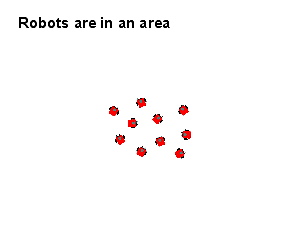
\includegraphics[width=0.3\linewidth]{../ui_experiment/slide_images/Swarm_Robot_Control_-_Unknown_Number_of_Robots_0001.png}}
		\fbox{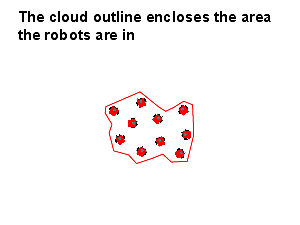
\includegraphics[width=0.3\linewidth]{../ui_experiment/slide_images/Swarm_Robot_Control_-_Unknown_Number_of_Robots_0002.png}}
		\fbox{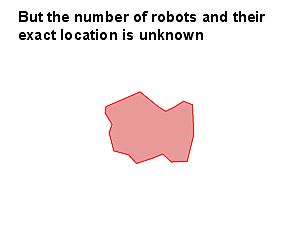
\includegraphics[width=0.3\linewidth]{../ui_experiment/slide_images/Swarm_Robot_Control_-_Unknown_Number_of_Robots_0003.png}}
	\end{subfigure}
	\caption{Instructional slides for the unknown number of robots condition, showing cloud representation of robot swarm.}
	\label{instructional_slides}
\end{figure}

Participant comments may shed some light on the source of this intuition. 
One participant indicated during the study that they interpreted the corners of the polygonal cloud as possible robot locations, and so drew an idea of the scale of the swarm from the number of corners. 
The cloud has 11 corners, 7 convex and 4 concave, which is consistent with the estimated robot count. 
Another participant said their estimate was informed by the instructional slides preceding the test, which depicted a number of robots, the outline around them, and the resulting cloud, as shown in Figure~\ref{instructional_slides}. 
These slides depicted 10 robots, and so may have biased participants to expect that the cloud had 10 robots in it. 
However, multiple participants stated that the cloud represented an unknown number, or estimated more or less than 10 robots.

\section{Selection Behavior} \label{section:Selection_Strategy}

At the end of the experiment, users were shown an image of a robot swarm, with a dotted line around it depicting a finger drag path around some of the robots. 
The users were told that the intent of this gesture was to select robots, and asked to indicate which robots in the image were selected, or in the unknown number of robots case, whether the gesture selected all of the robots or left any out. 
Users in the single robot case were shown the selection image with ten robots in it, because the with one robot, there are not enough robots to have a selection that may exclude some robots and include others. 

\begin{figure}
	\centering
	\begin{subfigure}{0.48\textwidth}
		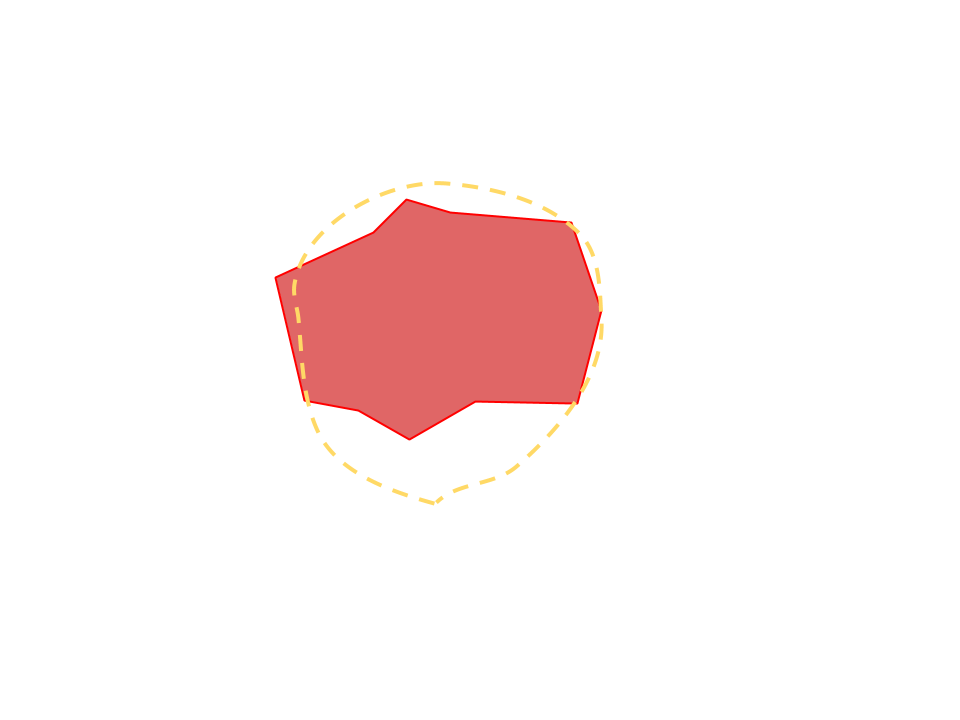
\includegraphics[width=\linewidth]{../Selection_Fuzz_X.png}
	\end{subfigure}
	\begin{subfigure}{0.48\textwidth}
		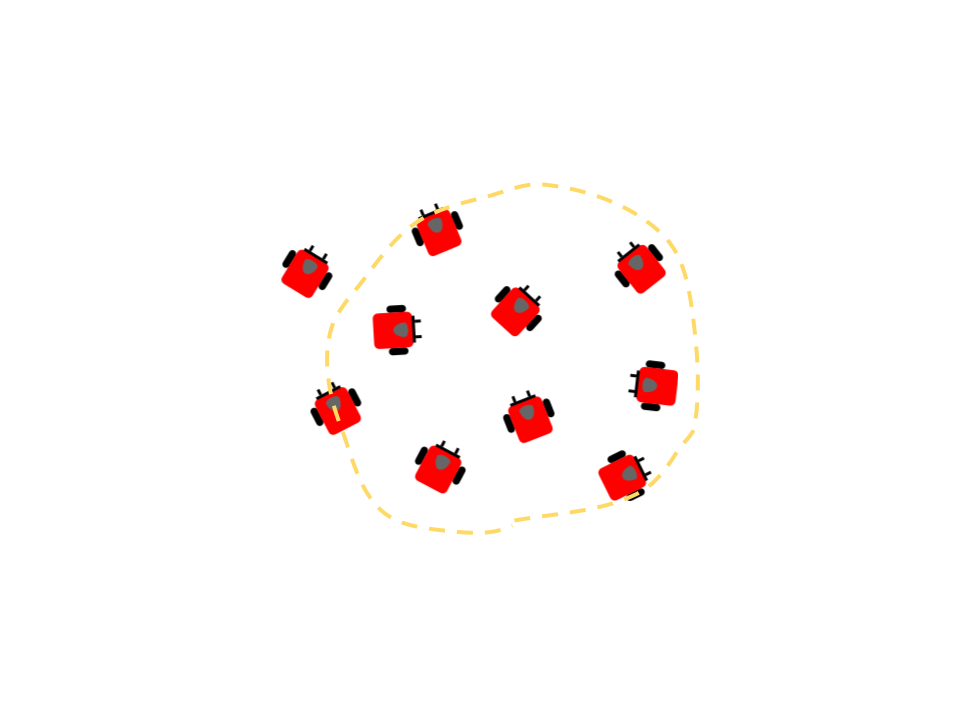
\includegraphics[width=\linewidth]{../Selection_Fuzz_10.png}
	\end{subfigure}
	\begin{subfigure}{0.48\textwidth}
		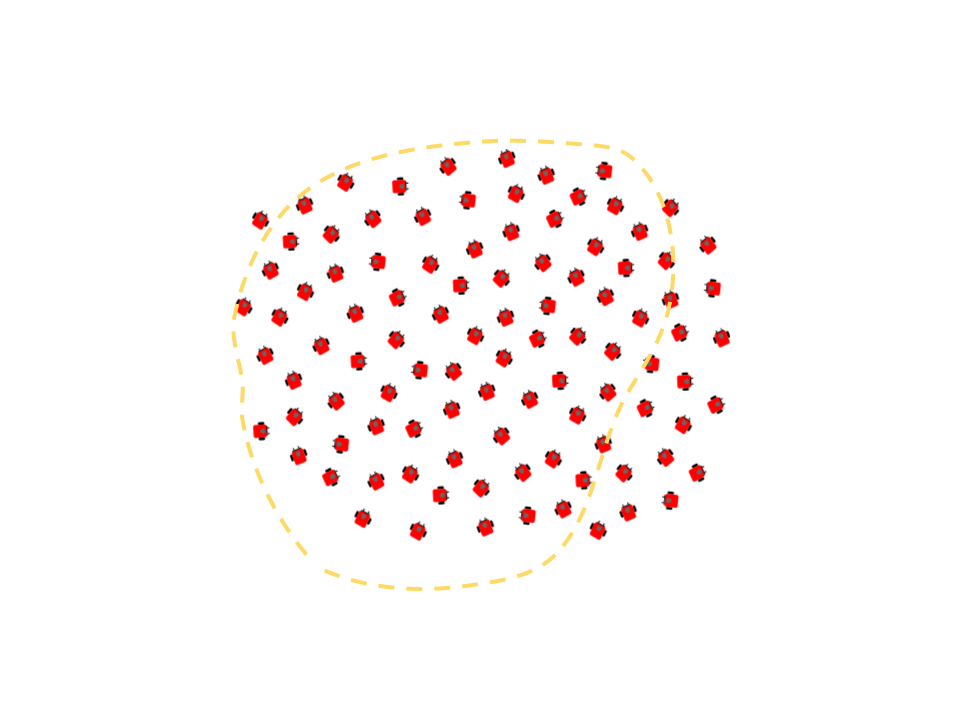
\includegraphics[width=\linewidth]{../Selection_Fuzz_100.png}
	\end{subfigure}
	\begin{subfigure}{0.48\textwidth}
		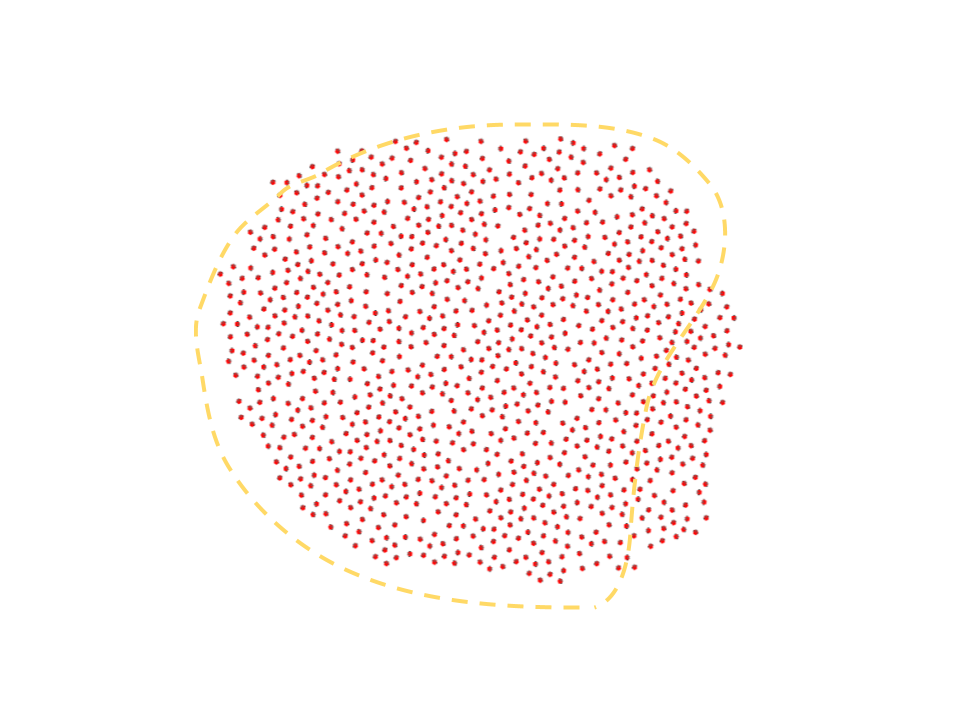
\includegraphics[width=\linewidth]{../Selection_Fuzz_1000.png}
	\end{subfigure}
	\caption{Images for selection strategy question.}
	\label{strategy_question}
\end{figure}

In the unknown number of robots case, 7 participants indicated that all the robots were selected, 3 of the participants indicated that some robots were left out, and one participant indicated that whether the selection included all of the robots could depend on the task. 

Because the 1 and 10 robot cases saw the same selection image, they are reported together. 
Twelve participants indicated that robots that were inside the selection or touched by the selection line should be considered selected. 
Two participants indicated that robots depicted with half or more of the robot inside the circle should be considered selected. 
One participant indicated that the robot half out of the circle should \emph{not} be selected. 
One participant indicated that robots on the border should be included or not included in the selection, depending on the task. %\todo{Three answers are missing, find those and fix}
One user indicated that only the first robot touched should be selected, which is consistent with control strategies that move each robot individually. 
The remaining three responses were not recorded due to researcher error. 

For the hundred robot case, 3 participants indicated that robots inside or touching the line were selected. 
Three participants said that robots should be mostly inside the line to be counted, with one participant stating that robots should be 80\% or more inside the line to count. 
Two participants indicated that robots should be more than halfway inside the line to be selected. 
One participant stated that only robots completely inside the line should be counted. %\todo{One answer missing, find and fix}

In the thousand robot case, 7 participants indicated that robots inside or touching the line should be selected. 
Two participants indicated that robots must be completely inside the line to be selected. 
One participant indicated that robots mostly inside the line should be selected. 

Overall, participants generally err on the side of inclusion, rather than exclusion of robots from selection.
If a user interface is required to include or exclude ambiguous elements from a selection, it appears that including ambiguous elements will satisfy users. 
User comments also suggested that ways to amend selections before further commanding the robots would be desirable.

\begin{table}
\begin{tabular}{ r r r r r}
	Condition & Completely inside & Half or more in & Touching line & Other\\
	\hline
	10 & 0 & 2 (10\%) & 12 (60\%) & 3 (15\%)\\
	
	100 & 1 (10\%) & 5 (50\%) & 3 (30\%) & 0 \\
	1000 & 2 (20\%) & 1 (10\%) & 7 (70\%) & 0\\
	\hline
	Totals & 3 & 8 & 22 & 2 \\
\end{tabular}
\caption{User responses for whether robots on the edge of a selection should be included. The unknown case is omitted because the relationship of individual robots to the line is not visible in that case. }
\end{table}

It is interesting to note that two participants, one from the unknown number of robots case, and one from the 10 robot case, said that in cases of ambiguous selection, the system should add or remove robots from the selection based on the task. 
As the system cannot predict the task it is about to be commanded to perform, it is likely best to err on the side of selecting too many robots, rather than too few. 

\section{NUI Metaphor Failure}

During this experiment, there were some cases where the users expectations of what was possible in the interface indicated a sort of ``metaphor failure" in the user interface. 
Natural User Interfaces, of which multitouch screens are an example, are supposed to be able to leverage users' understanding of the physical world, and how objects behave in it, to build affordances for objects on the screen. 
For example, a volume knob can be displayed as an actual knob, and the screen can react appropriately to attempts to rotate the knob. 
However, people know that the objects on the screen are not knobs, switches, and so on, but pictures of those things, drawn by the computer. 
As a result, the affordances are mixed. 
The knob may afford turning, but it also affords dragging around the screen or deletion, which a knob on a real radio does not afford. 

In this study, users were tasked with stopping the robots, which had begun to move around a wall to a target area. 
One user dragged the wall in front of the robots, and another user asked if they could move the wall. 
The wall was intended to represent an actual wall, which does not afford moving in the physical world, but it was represented in the experiment as a thick black line. 
It may be that the users would have not attempted to move the wall if it was more clearly represented as e.g. a stone or brick wall, and so had connotations of excessive weight. 
On the other hand, the users may have regarded it as what it actually was, an image of a wall on a computer screen, and decided that since images can be moved around the screen, the wall image can too. 
Attempting to experimentally determine if the representation affects how the user interacts with the wall would require an experiment better designed to examine that affordance, as out of 50 participants, only 2 even mentioned the idea of moving the wall.


% !TeX root = ams_thesis.tex
\chapter{UI Design and Implementation}

In order to convert the user gestures collected in the gesture collection experiment into a user interface, a subset of the gestures was selected to support the majority of the user-defined gestures. 

In some cases, the user defined gestures were ambiguous, either across users, or with a user across tasks. 
Where design decisions were made to work around these ambiguities, they are described. 

\section{Selection of Gestures for Control of Swarms}

\begin{figure}
	\centering
	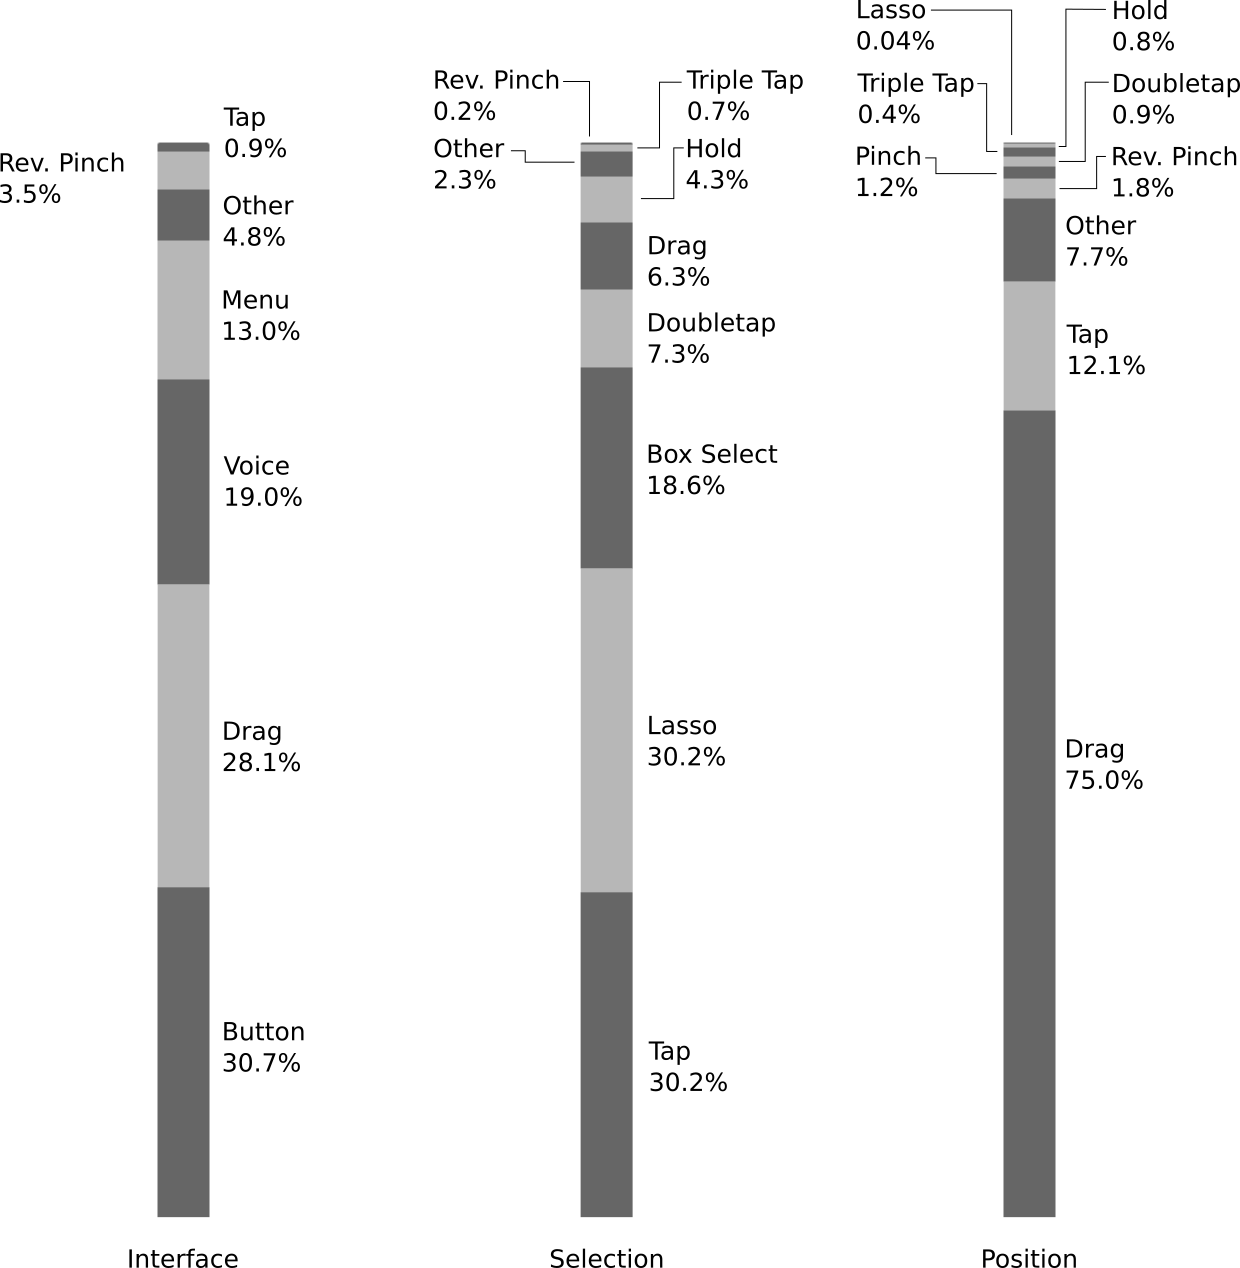
\includegraphics[width=\linewidth]{../thin_grey_text.png}
	\caption{Motion, selection, and UI gestures.}
	\label{fig:select_ui_move_breakdown}
\end{figure}

For position commands, drag, tap, and ``other'' would cover 94.8\% of the gestures. 
Unfortunately, the ``other'' commands are not a single gesture, but include a diverse collection of gestures, such as pushing with the side of the finger or making a picking-up, carrying, and setting-down motion over the screen.
As a consequence, attempting to implement all the gestures in the ``other'' category would add significant complexity to the gesture recognition in order to support gestures that were rarely used. 
Many of the ``other'' gestures were also not recognizable by a multitouch surface, such as the user dividing the robots by parting their hands as if opening a bag in the air above the surface. 
Since it does not contact the multitouch surface, such a gesture cannot be recognized without additional hardware. 
If all forms of tap are considered the same when used as position commands, taps make up 14.2\% of the position commands, and together with drag, cover 89.2\% of the position commands. 

Lasso was used as a position command by one user, who used it to command the robots to disperse in the ``disperse'' task. 
The user noted that the direction of the lasso disambiguated it from lasso as selection, so lassoing clockwise would select robots and lassoing counterclockwise would disperse them. 

Achieving 90\% recognition of the most common UI widgets would include buttons for special functions, handwriting recognition, voice commands, and other menus on the screen (totaling 90.8\%). 
However, a successful menu-based UI would not be composed simply by taking the sum of all of the user interface designs suggested by users, as there would be significant redundancy in the UI commands, and in ways of bringing up the UI for interaction. 
Instead, the tasks that the users invoked the UI in most often were examined, and the requested UI functions were considered for inclusion.

Both voice commands and handwritten commands together account for 47.1\% of the user interface elements used.
While the broad categories make up nearly half of the UI elements, the individual uses of the gestures did not display a significant unity within the broad categories.
One user used symbols drawn over the swarm as commands, so a circle drawn within the swarm area meant ``patrol", and would be followed by an indication of the area to be patrolled. 
Another user wrote commands, such as writing out ``0.5" to indicate that robots should divide in half, ``SQ'' to indicate that they should form a square, or ``C $\rightarrow$ A" to indicate that the crate (C) should be moved to area A. 
The majority of the drawn commands were attributable to a single user, but two users drew an `X' over the defective robot in the ``mark defective robot'' and ``remove defective robot'' tasks and two users used an `X' and an `S' in the ``stop the robots'' task.

The selection of a set of handwritten commands that would be usable for a majority of users would be a task at least as difficult as finding a user-defined set of gestures.
In addition to the set of English letters, the interface would have to consider symbols such as arrows, and apparently decimal numbers as well. 
The experiment described in this thesis did not collect sufficient examples of handwritten commands to extrapolate a useful control scheme from them.
Because of this lack of information, and the fact that most handwritten commands were proposed by a single user, the resulting interface does not contain support for handwriting recognition and symbol interpretation.  

Interestingly, voice commands were similar to both handwriting, in terms of distribution of user choice, and gestures, in terms of syntax. 
One user used voice commands for all tasks, but ten users also used voice commands for at least once. 
The distribution of voice commands is like the handwritten commands, in that one user used handwritten commands frequently, but a few other users used a few of them for some tasks.
The accidental biasing of users towards use of voice for formation tasks was discussed earlier. 
In addition, two users stated that they would like to have a vocal stop command for the ``stop the robots'' task, because it could be issued quickly and without having to accurately touch the moving robots. 
These users did not issue other voice commands, as the other tasks were not perceived to be as urgent as the ``stop the robots'' task. 

\begin{table}
	\centering
	\begin{tabular}{l l}
		Task & Uses of Voice Commands\\
		\hline
		line & 5\\
		square & 4 \\
		crate dispersed & 3 \\
		divide color mix & 3\\
		stop & 3\\
		crate & 2\\
		move a & 2\\
		disperse & 2\\
		merge & 2\\
		split & 2\\
		patrol a & 2 \\
		divide & 1 \\
		divide color 1 & 1\\
		divide color 2 & 1\\
		move wall & 1\\
		remove & 1\\
		mark & 1 \\
		patrol screen & 1\\
	\end{tabular}
	\caption{Use of voice commands by task. The use of high numbers of voice commands for the formation tasks, line and square, was likely biased by the text of the instructional slides. }
\end{table}

The syntactic similarity between the voice commands and the gesture commands is because the gesture commands frequently take the subject-verb-object ordering of spoken sentences. 
Some parallelism in the structure of spoken commands and gestures is  unsurprising, as in human-to-human communication, vocal expressions and gestures are theorized to arise from the same internal representations \citep{mcneill1985so}. 
For example, selecting the robot group indicates a subject, and drawing the path indicates the verb (``go this way"). 
Objects are optional or implied, as going to a location does not have a clear object that the robots are instructed to act upon. 
In some cases, the subject is implied as well.
For example, some users would make gestures intended to move the robot group as a whole by simply dragging the path, without selecting the subject first. 
In such a case, the implied subject was all of the robots. 
This sort of implication is more complex than simply assuming that if no robot is selected, all of the robots are the subject. 
Some users divided the robots into two groups by drawing a dividing line, and then dragging two paths, one to one side of the screen and the other to the other side of the screen. 
In this case, the implied subject was the half of the robots on the same side of the dividing line as the drag, but no selection gesture preceded the positioning drag to indicate this. 

%The idea of having a hidden menu that was dragged in from an edge of the screen or came up after some form of invocation, such as tap-and-hold, was rejected because such menus do not admit exploration. \todo{cite something on explorability/discovery of menus}

Reverse pinch was used as an interface command to zoom in or out of the view of the robots. This was done in the ``mark defective robot'' and ``remove defective robot'' tasks. 
The user who made this gesture was in the 1000 robot case, and stated that they wanted to zoom in because the defective robot was a small target and close to other robots. 
There was no explicit zoom or change of viewpoint task, but users expected the functionality when they had to interact with a small target.

To accommodate 90\% of the user gestures for selection, recognition of tap, lasso, box select, doubletap, drag, hold, and ``other'', totaling 91.9\% of the selection gestures.
As discussed above, the ``other'' category is not practical to implement. 
If, instead, all forms of tap are considered the same for purposes of selection, they comprise 42.5\% of the selection gestures, and together with lasso and box select, cover 91.3\% of the selections. 

Drag as a selection gesture refers to the user placing their finger on one robot, and then dragging it from robot to robot, adding each touched robot to the selection. 
It is ambiguous with the position drag, where the user places their finger on a robot and then drags a path for the robot to follow, although the distinction could be made by having a path that intersects multiple robots become a selection, rather than a position command. 
Unfortunately, this attempt at disambiguation would itself become a source of problems if the user attempts to move the entire swarm by placing a finger in the middle of it and dragging to a new location, as it is likely they would intersect more than one robot as their finger leaves the swarm.

\section{Ambiguities in Gesture Commands}

As discussed briefly in the previous section, some combinations of gestures selected by the users were ambiguous. 
This is to be expected, as the users did not know all the tasks in advance, and so might use a gesture in one task that they then felt was better suited to a later task.
The users might also not regard all the tasks as having to use a consistent and unambiguous representation for each gesture, or not remember all the gestures they had previously used. 
However, for automated conversion into programs, it is important that a sequence of gestures have some way to be unambiguously recognized. 

In the line formation tasks, some users selected the robots and then drew a line to indicate the location of the line formation. 
If the line formation started at the same location as the robots, this gesture sequence is the same as the selection and drawing a path sequence that was frequently used to indicate that the robots should move as a group along the path. 
If the line formation started elsewhere, it could be disambiguated, because motion along a path almost always started on or near the selected robots.  
The user drawing a line over a group of robots could be interpreted a number of ways: as a dividing line, as a box selection, as a path for a single robot to follow, as a path for a group of robots to follow, and as the location of a line formation.

Because a number of other, more explicit commands are available for dividing robots into groups, such as moving one group away from the other, the division line interpretation was rejected. 
A line drawn over robots is treated as a box selection, unless it begins on a single robot. 
In that case it is interpreted as a path for that robot to follow. 
For the purposes of this work, beginning ``on'' a robot was defined as the beginning of the line being within 80 pixels of the location of the robot on the screen. 
80 pixels was selected because it is the approximate width of a human finger on the screen used in this work. 
Obviously, this distance will vary with the resolution of the screen, but the mechanism for obtaining the resolution and physical size of attached screens varies with operating systems, and is outside of the scope of this work, aside from noting that this parameter may vary.

Similarly, some users divided the robots into two groups by drawing a line separating the groups.
Typically, this line started outside the group and passed through it, so it could be disambiguated from instructing the robots to move along the line.
Unfortunately, it would be difficult to separate it from drawing a line for the robots to move to in order to create a formation.

To command the robots into a square formation, especially in the dispersed cases, many users simply drew the square formation over the robots.
If a lasso select is also available, some distinction must be made between the lasso select and the square formation when they are both drawn over the robots, as they are both closed forms drawn over the robots.
One possible method is to look for peaks in the distance from each point on the perimeter of the gesture to the centroid of the gesture. 
A square would have four peaks, while a circle would have no obvious peaks. 
However, this sort of recognition means that a square lasso select, or an arbitrarily-shaped lasso select that happens to have four peaks, would get misinterpreted as a formation gesture, while a command to get into a circular formation would be interpreted as a lasso selection. 
It would be preferable to be able to make arbitrary formations, and arbitrarily-shaped lasso selections, and have them be disambiguated by some other method. 
One method that users proposed was to have a ``draw formation" button, which would then cause the next form that the user drew to be treated as the perimeter of the formation. 
Some users also held one finger down at the start of the formation, while tracing the perimeter with the other finger. 
Using a multi-finger gesture has the advantage of not adding UI elements, but is not easily discoverable by a user examining the UI. 

In order to patrol area A or the screen border, users frequently dragged the robots as if issuing a basic motion command. 
Some users indicated that there would have to be an additional signal to the robots to keep moving on the patrol route, once it was assigned, but there was not an agreement as to what that command should be. 
Of the users who indicated a need to convey that the swarm keep patrolling, some repeated the patrol route drag multiple times, others ended the gesture with a tap or triple tap, still others used the direction of the patrol route drag (clockwise or counterclockwise) to separate following the path once from continuously following it. 

Some users reused gestures for different purposes, such as tapping a robot to select it, but also tapping a robot to remove it.
Because 30.2\% of the selection gestures were taps, it was decided that selection, which occurs often, would be done by tapping, while removal of a robot, which is rare, would be performed by a different action. 

\subsection{Implicit Selection}

The distinction between interpreting a line drawn over robots as a command for one robot to follow versus a command for multiple robots to follow may depend on the number of robots present.
As seen in section \ref{section:Selection_Gestures} the use of selection gestures was low in the 1000 robot case, but and much higher in the 10 robot case, implying that with a large robot group, it might make sense to default to using all robots if none are selected. 
The interface could even change depending on the number of units being commanded, with small groups requiring that all robots be selected before a command can be applied to them, and larger groups defaulting to issuing the command to all robots if some subset has not already been selected. 
However, care must be taken to avoid learning effects. 
If the user has previously been exposed to a condition where the system defaults to selecting all robots, they may develop an expectation that other conditions behave the same, and neglect to select robots, resulting in incomplete commands (or commands being applied to no robots). 
Interestingly, the opposite case, where the user makes a selection of all the robots, but it is not actually required because it is the default behavior, does not result in a surprise for the user. 
Because the failure mode encouraged by a system that requires explicit selection is less surprising than one that has implicit select-all, the system was developed to require selection to issue a command to multiple robots. 
As described above, issuing a command to a single robot may be done without selecting it first, by beginning the desired path on the robot. 

\subsection{Gesture Complexity}

The gestures used by the users could be divided between selection and position gestures, within which there was a great deal of agreement, and more complex actions, such as patrol, formations, picking up or moving objects, removing robots, and selection by color. 

For selection, if the system accepts taps (of any form), lasso, and box select, 91.3\% of the user selection gestures are covered. For position, tapping (again, of any form) to set goals or way points and dragging paths will cover 89.2\% of user position gestures.

Because the more complex tasks had higher variety of gestures that could be used to convey the user intent, as well as some users performing the more complex tasks by repeated selection and position gestures, attempting to handle this variety of gestures leads to two problems with the discoverability of the interface. 

First, since each of the gestures was chosen by a smaller number of the users, some training must be performed to inform users who would not have chosen that gesture. 
This training could be done with a ``cheat-sheet'' that users could pull up for reference, or an animated introductory tutorial sequence. 
These options are both less desirable than having the system be, as much as it can be, self-explaining. 
They separate the training of the user from the user's interaction with the interface, rather than having the interface make clear what can be done.

Second, if a large percentage of the gestures for the more complex tasks were implemented, in order to provide high coverage of the various options that users chose to perform those tasks, there would be a large set of gestures that have very specific meanings. 
Increasing the set of gestures that the system recognizes increases the chances for ambiguities, where the same gesture was selected for multiple roles by different users, and for errors, where the system misinterprets one gesture as another. 
This interferes with discoverability, as the system may react in different ways to what the user felt were the same actions, confounding the user's ability to learn a mapping between their actions and the results that the system produces. 

As a result, the complex tasks were assigned to buttons on the user interface. 
The use of buttons is more discoverable, as the button simply says on it what it does. 
Buttons do obscure some of the camera view that forms the main part of the user interface, but this problem is not as severe as it might appear. 
The area the robots operate in is either bounded or unbounded.
If it is bounded, it either fits on the screen or does not fit on the screen, and if it is unbounded, it does not fit on the screen.
If the area the robots are in does not fit on the screen, the user likely views it by panning or zooming in and out, and so can pan or zoom so that the area covered by the buttons is not an area that they have to interact with to perform a task. 
If the area the robots are displayed on and interacted with in does fit on the screen, it can be shrunk slightly, and the buttons can be placed so they don't cover the interaction area. 
In either case, the design of the interface can accommodate a few buttons without seriously harming the user interaction, although the unchecked proliferation of buttons could lead to design difficulties. 

\section{Termination of Commands}

Some of the potential gesture commands, such as selection of a group of robots followed by tapping waypoints for them to follow, do not have a clear termination, as the system cannot tell if the user is done tapping waypoints, or simply has not tapped the next one yet. 
One potential solution to this problem is to attempt to parse the user command once enough time has elapsed since the last gesture received. 
Using a timeout to commit the command was rejected for two reasons. 
First, the timeout can result in the system beginning to take an action that the user did not want. If the timeout is too short, it could result in a program being transmitted to the robots before the user is done specifying it. 
If it is too long, it may never be triggered, and so all of the user's gestures could be gathered into one, potentially untranslatable, program. 
Second, the timeout is could be invisible. From the user's perspective, this causes the system to appear to begin acting at random, which is undesirable. 
The timeout could be made visible, using a countdown timer, which may then make the user feel pressured to act. 

In order to avoid having the system act prematurely, the system treats a doubletap on open space as an ``end of command" signifier.
If the hardware used in the system were capable of detecting it, the user placing their hands in their lap or away from the screen could also be used as a signifier that the user has completed entry of their command. 
Most users moved back from the screen slightly and removed their hands from the volume above it once they were finished issuing their command, and no users were observed to rest their hands on the screen while not issuing commands. 
However, this behavior may have been a consequence of the particular arrangement of the screen and user seating, so further work would be required to determine if it is a sufficiently robust indication of command completion. 

In addition to doubletaps, there are limited instances where it is safe for the system to assume that the user's command is complete. 
Because commands are generally of the form subject-verb-object, a new subject begins a new command. 
The exception to this rule is tap selections, which some users used to select multiple robots by sequentially tapping on them. 
Tap selections are accumulated until a gesture other than a tap selection is entered.
After a non-tap action is entered, a new selection gesture will begin a new command. 

\section{Acceptable Command Sequences}

The commands that use buttons are Patrol, Make Formation, Move Object, Remove Robot, and Select Group. 
The text of the buttons is written as a verb phrase, as the buttons take the place of the verb in the subject-verb-object (SVO) structure. 
To preserve the SVO ordering, the command parser expects a subject, specified by a selection gesture, a verb, expressed by a button, and then an object, expressed by another gesture. 

For Patrol and Make Formation, the ``sentence'' reads somewhat like ``These robots, Patrol/Make Formation, this location/shape". 
The selection is performed, then the button pressed, then the location or shape is specified. 

In the Move Object command, the sentence is more complex, as both an object to be moved and a location to move it to must be specified. 
The sentence would read as ``These robots, Move Object, this object, to here". 
This structure is somewhat in conflict with the most common user strategy to move the crate, which was to surround the crate with robots and move the robots, and also in conflict with the second most common strategy, which was to move the crate, with no reference to the robots. 
The decision to differ from these strategies was undertaken for a number of reasons. 
The first is that moving the crate with no reference to the robots implies that the subject of the sentence is all of the robots. 
As discussed previously, implicit selection of the entire swarm has a high potential to surprise the user, especially if the behavior changes across swarm sizes, while requiring explicit selection does not. 
The second is that unless the system is aware of which objects in the environment are movable and which are not, there is no way to disambiguate a command to surround an object, and then leave it to go to another location, from a command to move the object by surrounding it.
This level of knowledge about a novel environment may not be possible to obtain in real-world situations. 

The Select Group and Remove Robots buttons are not commands to the robots. 
They are commands to the system. 
Select Group selects robots by some common feature (in the user test, common group membership was depicted by color). 
Remove Robot instructs the system to mark a robot or robots as not to be used, and so they are excluded from having commands issued to them. 
The system is the implied subject of the sentences ``[System], Remove Robot, these robots'' and ``[System], Select Group, these robots''. 
Implying the subject of a command to the system is acceptable in a way that implying robots as a subject is not, because there is one control system, and so the subject is not ambiguous. 
The interface can be viewed as similar to a desktop computer, where it is generally assumed that commands invoked through that computer's UI are for that computer to do. 

The commands that are not invoked through buttons are the positioning commands, to move single robots or groups. 
The division between buttons and ``pure'' gesture commands was made because there was higher agreement between users on the basic movement commands than on the more complex commands. 
Additionally, some users implemented the more complex commands by sequences of basic motions. 
This was especially apparent in formation commands with lower counts of robots, where some users issued individual movement commands to each robot, which ended at a location within the formation. 

Positioning commands consist of a subject and a verb phrase gesture that reads as ``These robots, go here". 
However, there are a number of ways that these can be expressed. 
The selection can be by any of the selection methods. 
The position commands can be by tapping a location, or by dragging a path for the robots to follow. 
However, this raises the possibility that the dragged path is a line or loop over other robots, and so resembles a group selection. 
There are two possible ways to treat this sequence. 

The fact that there is an end-of-command marker, the ``period'' at the end of each sentence, means that the user could make a sequence of taps on robots, lassos, and box selection gestures, ending with either something that could be a path, a lasso, or a box selection and then the end-of-command marker. 
The system would then interpret the last lasso or box selection as a path, and so the whole command as a sentence with a compound subject, ``These robots and this robot and..., go here''. 

The other possibility is having each selection create a new command. 
If that is the case, it becomes impossible to patrol an area with robots in it, or have one robot move through a group of robots, as those gestures are a lasso or box selection that starts a new command. 
The exact ambiguity is not between all selections and path commands, but between group selections and path commands.
Tap selection of single robots is unambiguous, under the assumption that collisions are bad, and so it is never desirable to command one robot to another robot's exact location. 

This raises the possibility of a third selection method, where single/tap selects can be chained to select multiple robots. 
If tap selections are allowed to chain, it does create an instance of a selection not terminating an old command and starting a new one, creating an inconsistency with the rule that starting a new selection begins a new command, and so implicitly ends any previous command.

If tap selections are not allowed to chain at all, then tapping multiple robots one after another only selects the last one, and results in a sequence of incomplete programs consisting only of selections. 
It also eliminates a behavior that some users did show, selecting a small number of robots by tapping on the individual robots. 
Because it admits very detailed multi-selection and supports a selection style that users chose, tap selections were allowed to chain with each other, but not with other selections. 

Having selections end the previous command and start a new one, combined with the existence of lasso selection and box selection, adds some complexity to attempts to send the robots on a path that looks like a lasso or box selection. 
Determining whether a loop-like gesture or a box-like gesture is intended as a path in the previous command, or the beginning of the next command, depends on whether it is immediately followed by an end-of-command gesture. 
If the resulting stack of gestures consists of some form of selection, a box or lasso selection, and then an end-of-command, then the box or lasso selection can be replaced by a path gesture, and the program becomes valid. 
However, if the stack contains some form of selection, a box or lasso selection, and e.g. a path gesture, then the first selection is an erroneous program consisting only of selection, and can be dumped from the stack. 

Similar heuristic rewriting of the stack could be extended to e.g. remove erroneous waypoints resulting from triple-tapping instead of double-tapping to end gestures, but adding these sorts of heuristics poses something of a threat. 
There exists some rewriting of the user input that will eventually result in an acceptable sequence of gestures, even if it is a complete replacement of all of the user input. 
However, at some point, the meaning of the rewritten stack will deviate from what the user intended. 
While using such a stack of commands will result in the generation of a program for the robots, it will not be a correct program, from the user's point of view. 
In such a case, it would be better to have the parsing of the user input fail. 
The determination of what level of alteration of the user input is acceptable is not the core subject of this research, but is an interesting question. 

\section{Simultaneous Actions}

Expecting a sentence-like form for commands does not take as much advantage as it possibly could of simultaneous actions. 
The multitouch surface used in this work can track 20 points at once, and some surfaces can track even more. 
As a result, the hardware will allow users to, for example, perform selections with both hands at the same time and then draw a path with each hand. 
Sentences, on the other hand, are generally spoken serially, instead of in parallel, so the analogy to language does not provide a convenient heuristic for determining which subjects go with which verbs.
While two selections performed at the same time will overlap, one is almost certain to finish before the other, and so could be interpreted as a selection following another selection. 
Even if overlapping selections result in two groups both being selected independently, if the user then taps two goal points and ends the command, the result is ambiguous. 
If the two goals were tapped one after the other, they could each be a goal for one selected group, or a sequence for both selected groups to visit.
If the two goals were tapped at the same time, perhaps they are each a goal for one group, but which group should go to which goal is unspecified.  
While there are heuristics that could be used to guess user intention in these cases, such as always dispatching the closest selected group to a given goal, the system does not have the information to properly guess the user's intent.

However, two-handed gestures accounted for only 5.037\% of the gestures used, if the motion of each hand is counted as a separate gesture. 
As a consequence, the loss of the ability to perform simultaneous gestures, in a single-user context, does not result in a large loss of functionality.
In a multi-user context, it would be desirable to have users be able to perform interactions simultaneously, but such an extension would also require additional information to associate contact points on the multitouch surface with particular users. 

Abandoning the use of simultaneous gestures also allows the unambiguous use of the scatter gesture for triggering dispersion. 
If simultaneous gestures are allowed, then performing the scatter gesture over a group of robots is detected by the system as several simultaneous attempts to drag robots and draw paths at the same time. 
If the gesture is is performed over open space, it is detected as 4-5 paths being drawn at the same time. 
With simultaneous gestures, the command sentence selects some group of robots and sends them multiple paths to possibly follow, with no order in which they should be followed. 
However, without simultaneous gestures, the multiple contacts can be combined as a single scatter gesture. 

\section{Representation Of The Command Language}
The command input language can be defined formally, given the constraints above. The Augmented Backus-Naur Form (ABNF) description of the language is given below. Using the scatter gesture for dispersion is indicated in ABNF as 4*5(dragRobot|path) to require that there be at least four and at most five fingers used to make the gesture. 
An alternate approach would be to have the gesture detection coalesce paths and robot drags that were close enough in space and overlapping in time, and present them as a single ``scatter'' gesture. 

%Thanks to https://tex.stackexchange.com/questions/308726/place-newline-in-backnaur-package
\newenvironment{bnfsplit}[1][0.7\textwidth]
{\minipage[t]{#1}$}
{$\endminipage}

\begin{bnf}
\bnfprod{sentence} 
	{\bnfpn{cmd} \bnfts{endCmd}}\\
\bnfprod{cmd}
	{
		\begin{bnfsplit}
		\bnfpn{patrol} \bnfor \bnfpn{makeFormation} \bnfor \bnfpn{moveObject}\\
		\bnfor \bnfpn{removeRobot} \bnfor \bnfpn{disperse} \bnfor \bnfpn{goHere} 
		\vspace{2mm}
		\end{bnfsplit}
	}\\
%``These robots, Patrol, this area". 
\bnfprod{patrol}
	{\bnfpn{selection}\bnftd{Patrol}\bnfpn{path}}\\
%``These robots, Make Formation, this shape". 
\bnfprod{makeFormation}
	{\bnfpn{selection}\bnftd{Make Formation}\bnfpn{path}}\\
%``These robots, Move Object, this object, to here". 
\bnfprod{moveObject}
	{\bnfpn{selection}\bnftd{Move Object}\bnfpn{selection}\bnfpn{path}}\\
%``[system] Remove Robot, these robots''
\bnfprod{removeRobot}
	{\bnftd{Remove Robot}\bnfpn{selection}}\\
%``These robots, scatter"
\bnfprod{disperse}
	{\bnfpn{selection}\bnfpn{scatter}}\\
\bnfprod{scatter}
	{4*5(\bnfts{dragRobot} \bnfor \bnfts{path})}\\
%``These robots, follow this path"
%``These robots, go here"
%``This robot, go here"
\bnfprod{goHere}
	{\bnfpn{selection}\bnfpn{path} \bnfor \bnfts{dragRobot}}\\
\bnfprod{path}
	{\bnfts{tapWaypoint+} \bnfor \bnfts{dragPath}}\\
%``[system], Select Group, these robots''. 
\bnfprod{groupSelect}
	{\bnftd{``Select Group"}\bnfts{tapSelect}}\\
\bnfprod{gestureSelect}
	{\bnfts{tapSelect+} \bnfor \bnfts{boxSelect} \bnfor \bnfts{lassoSelect}}\\
\bnfprod{selection}
	{\bnfpn{gestureSelect} \bnfor \bnfpn{groupSelect}}
%	\\	
%\bnfprod{robotList}
%	{\bnfts{"["} \bnfpn{robotID}+ \bnfts{"]"}}\\
%\bnfprod{robotID}
%	{\bnfpn{INTEGER}}\\
%\bnfprod{pointList}
%	{\bnfts{"["} \bnfpn{point}+ \bnfts{"]"}}\\
%\bnfprod{point}
%	{\bnfts{"("} \bnfpn{x} \bnfts{","} \bnfpn{y} \bnfts{")"}}\\
%\bnfprod{x} 
%	{\bnfpn{DECIMAL}}\\
%\bnfprod{y}
%	{\bnfpn{DECIMAL}}\\
%\bnfprod{INTEGER}
%	{\bnfts{("0".."9")+}}\\
%\bnfprod{DECIMAL}
%	{\bnfts{"-"}? \bnfpn{INTEGER} \bnfts{"."} \bnfpn{INTEGER}}
\end{bnf}

The terminals of the language are the gestures recognized by the system, that is to say selection by tapping, box, or lasso, waypoint tapping, dragging a robot along a path, dragging a path, dispersion, the buttons and double-tapping to end a command. 
The terminals in italics in the ABNF representation are the names of the buttons. 

% !TeX root = ams_thesis.tex
\chapter{Implementation of Swarm Actions} \label{chapter:Implementation_of_Swarm_Actions}

The user interface may be able to drive the re-imagining of the robots as a unified swarm, and so alter the user's interaction with the swarm, by depicting the group in different ways \citep{manning2015heuristic}.
The base case is to simply display all the units as individuals, but this may not be useful for the operator \citep{coppin2012controlling}. 
Other approaches include an amorphous shape covering the area occupied by the swarm, an amorphous shape with density shading and motion arrows, the fields of influence for leaders in the swarm, and the web generated by the flow of information within the swarm. 
Considered as a whole, the swarm has properties, such as center of gravity or flock thickness, that do not exist in individual robots. 
Views of these properties may assist the user, for example in determining what areas have insufficient robot density for a thorough search operation. 

The information available to the user through the UI also implies the availability of certain information within the system. 
The distinction between UI representations of the swarm that display each robot as an individual robot versus those that display a cloud or amorphous shape in the area occupied by robots is the most obvious example. 
A system that displays the location of each robot must actually have localization information about each robot.
The presence of this information in turn implies that the localization information can be used to plan the actions of each robot, which in turn affects the structure of the programs generated for each robot. 

For example, if the task assigned to the swarm is to surround a fixed point, and localization information is available, then each robot can be given a program that instructs it to move towards a known location, based on its current known location.
Even if the robots cannot determine their location, but the UI and program generator have it, the robots closest to the point can be assigned programs that cause them to act as beacons, while all the other robots are assigned programs to wander until they see a beacon and then move towards it. 
If, instead, neither the robots nor the program generator have information on the location of the robots, then all of the robots can be assigned programs that instruct them to wander until they detect the target point, and then act as beacons, at which point the overall behavior of the system returns to the previous example.

In the most extreme case, neither the robots nor the user interface have any information about the location of the robots. 
As a consequence, the system could not display the individual robots situated in relation to each other on some form of map. 
This extreme is outside the scope of this work, as it is more suited to an interface that permits the provisioning of the robots with a description of the target point. 
A method for providing such a description through multitouch gestures is likely to be more tedious than other approaches, e.g. summarizing desired sensor precepts or including an image of the target area for the robots to recognize. 
However, if the user task is expressible in terms of the overhead view of the area, the user interface could simply allow the user to issue commands that are situated in that view, such as rallying at a certain point or moving an object that is visible in overhead view. 
Without information about the robot positions, the user would not be able to watch the motion of the robots to see that the commands were being followed. 

All of the valid expressions possible in the command language should be converted into programs for the robots, or the user must be usefully informed as to why it was not possible. 
The synthesized program should result in convergence of the swarm's overall behavior to the desired result. 
Clearly, in a developing situation in the real world, success may become impossible, and so there is not a practical way to guarantee that a particular valid command sequence will result in a particular desired state of the world. 
However, certain minimum bounds on the problem may be able to be used to determine if a desired task is certain to fail. 

\section{Localization}

The initial vision for this work was to have minimal sensing and no localization. 
Minimal sensing results in a lower cost per robot, as it reduces the amount spent on sensors. 
Not relying on localization, especially localization via approaches such as GPS, which are easily blocked or interfered with, allows the resulting algorithms to be useful in situations where global localization is not available. 

However, a user interface that can display the swarm from an overhead view assumes that there is some form of localization, at least in terms of relative distances and bearings between the robots.
Without that information, the display of a group of robots in a way that matches their actual locations in the world is impossible, and displaying them incorrectly is likely to mislead the user. 
Even the unknown number of robots case assumes that the outer bounds of the swarm are at least approximately known. 

Fortunately for this work, there are a number of approaches to creating a local coordinate frame using robots with relatively simple sensors. 
A local coordinate system can be created by communicating agents with a limited, known sensing range but no other concept of distance \citep{bachrach2004experimental}.
One agent acts as a seed, and sends messages to its neighbours.
The neighbours propagate those messages, incrementing a hop counter in the message, and ignore messages with a higher hop count to stop the message from propagating backwards. 
As a result, each agent knows that its distance from the seed is at most the communication radius times the minimum hop count it has received. 
By using multiple seeds, each non-seed can calculate it's position based on trilateration to the seeds. 
Extending this method to use received signal strength as a proxy for distance, rather than the constant known sensing range, improves the accuracy of the approach.  
The Kilobot swarm uses a range-only sensor along with communication to create a local coordinate system \citep{Rubenstein795}.
A set of four stationary seed robots act as the origin of the coordinate system. As robots surround the four known robots, the new robot localizes from them and then begins broadcasting it's own position. 
Each new robot that joins the group uses trilateration to localize itself based on the robots that it can communicate with.

In addition to range-only approaches, bearing-only approaches to robot localization have been created, including an approach that uses the bearings to landmarks to create a vector field to drive the robot to a goal \citep{loizou2007biologically}. 
This approach is even able to guide an individual robot in the presence of moving landmarks. 
It does not, however, produce a coordinate frame that is shared among the robots, unless they somehow agree on the landmarks to use. 
A scale-free coordinate system can also be created using only bearing sensors and inter-robot communication, to arrive at a coordinate system that is shared among the robots \citep{cornejo2013scale}.
The addition of scale to such a system requires something beyond only bearing measurements. 
One way to do this is to use structure from motion (SfM) to estimate inter-agent distances, and use the measured distances to determine the scale for the network of robots \citep{spica2016active}. 
Alternatively, a pair of beacons of known location could provide the scale information required to convert scale-free coordinates into a metric coordinate system. 

Finally, systems that combine range and bearing information are common in swarm robotics \citep{arvin2009development, farrow2014miniature, caprari1998autonomous, mondada2009puck}. 
Systems with range and bearing can use trigonometry to calculate relative positions of other robots, and so can bootstrap a coordinate frame by using a method such as spreading inhibition to elect an origin robot, which then informs its neighbours of their positions in it's coordinate frame. The neighbours can then correct their position estimates based on communication with each other, as in range-based localization schemes, and inform their neighbours of their positions, propagating the coordinate system outward from the origin. 

As there already exist a large number of ways for robots to arrive at a local coordinate system without GPS or sophisticated sensors, the creation of a coordinate frame was determined to be outside of the scope of this work. 
Once the robots have developed a coordinate frame, the space the robots are in can be decomposed into a set of cells, and the program for the robots can be expressed in GCPR as checks on which cell the robot is located in and what the desired behaviour for the robot in that cell is. 
The desired behaviour for each cell is based on the user input on the interface device. Since the locations of the robots in the local coordinate system are known, and the location of the visualization of the robots on the user interface device is based on their positions in the local coordinate system, the user's input can be mapped into the local coordinate system to guide the robots. 
The combination of the spatial decomposition and the user input results in, essentially, a discrete vector field. 
By having the vectors in the field point towards a user supplied path, or along the path, the robots can follow the path using only their location in the local coordinate frame to guide them. 

Following the user-supplied path is important because it provides feedback to the user that the system is attempting to do what the user intended. 
In the simplest case, moving a robot to a target location, it could be argued that the thing that matters is that the robot arrive at the target location, rather than that it follow a specific path to get there. 
If a robot is in a bounded enclosure, and has a sensor that can detect when its goal is reached, the robot can reach the goal, or arbitrary close to it, by a random walk. 
If the robot can sense distance to the goal, it can find the direction of the goal by making a series of purposeful moves and samplings of the distance, and then go to the goal.
It could even approach the goal by performing a biased random walk. 
None of these approaches, however, would look to the user like the robot was following the path that the user provided, and so they are likely to confuse the user, leading to further control inputs as the user attempts to correct the robot. 
Additionally, the user's choice of path may be informed by knowledge that the user has, and that the robot may not be able to detect in the environment, such as areas that are inaccessible or dangerous to the robot. 
As such, the user's path selection can be viewed as an attempt to convey information about the desirability or utility of a given path to the robot, and so following the path given by the user is preferable to not following it. 

The space is decomposed into squares of uniform size. The size can be varied, but smaller squares result in a longer program for the robots and longer runtime for the decomposition algorithm. 
To determine the desired vector for a the cells of the spatial spatial decomposition, a multipass algorithm is used. 
The first pass assigns the vectors for those squares containing a point of the user specified path, or on the line between two points of the user path. 
Squares containing a point are assigned a vector pointing to the next point on the path. 
Squares between two points are assigned a vector pointing from the square center to the point closer to the end of the path. 
After this step, all points on the path have a vector pointing along the path. 
The second pass assigns to all squares neighbouring the end point of the path a vector pointed towards the end point of the path. 
As a result, the end point of the path becomes an attractor that robots attempt to reach. 
The third pass assigns to all squares that are adjacent to assigned squares a vector which is the average of all of the values of the assigned neighbors. 
This pass broadens the path so that it is greater than a single square wide, and ensures that the vector field around the path is smooth. 
The final pass is repeated until no square is assigned during a repetition. 
On each repetition, any square that is not assigned, but has assigned neighbors, is assigned the average of its neighbors and a vector from the center of the square to the closest point that is on the path. 
As a result, squares off the path drive the robot towards the path via the shortest route. 
When this pass is complete, every square of the decomposition of the space has been assigned a vector pointing in the direction that a robot in that square should move. 

The resulting decomposition can then be converted into a GCPR program by having each guard be a check on the position of the robot, and assignment of the robot's desired heading based on the grid square it is in.
A GCPR clause tells robots that are off their desired heading to rotate to that heading, and robots which are on their desired heading to move forward. 

Dispersion can be implemented in terms of vector fields as well. 
In the case of path following, every robot that was intended to follow the path would be issued the same decomposition of the space, but would follow different routes, as they start from different locations. 
To disperse the robots, each robot receives a different path, starting from their current location and moving to their new dispersed location. 
As described above, the robots can avoid each other while attempting to reach their new positions, and return to following their assigned paths once they are clear of each other. 
In implementation, the new locations were chosen by uniform random selection of points over the area the robots were in, but other approaches, such as positioning the robots so that each robot could communicate with at most two other robots, or on a regular grid in the local coordinate frame, would be amenable to the same implementation. 

These algorithms for path following and dispersion were implemented in ROS and tested in the ARGoS multi-robot simulator \citep{pinciroli2012argos}.

\section{Composition with Obstacle Avoidance} \label{section:Composition_with_Obstacle_Avoidance}

Reactive obstacle avoidance was initially added to the vector field program by only following the desired heading if the robot detects that it is not near any obstacles, and reacting to avoid the obstacles rather than follow the vector field if an obstacle is detected. 
This approach does have the weakness that the user can, for example, draw a path which passes through an obstacle. 
In a known environment, obstacles could be surrounded by repelling vectors, but in an unknown environment, this sort of command will cause the robots to approach the obstacle under vector field control, turn away from the obstacle until it is no longer visible, return to vector field control, and return to the obstacle. 

There exist a family of algorithims, called ``bug algorithms'', which provide complete path planning in a priori unknown environments with minimal sensing, under reasonable bounds, such as that the number of obstacles is finite and the goal is reachable. The bug family is large, and some of its members require sensing which may not hold in all conditions, such as location information or infinite-range distance sensing, but many do not. I-Bug, in particular, requires only the ability to detect a gradient which towards the goal and the ability to circumnavigate obstacles by e.g. wall following \citep{taylor2009bug}.

Generally, bug algorithms have two cases, the rules for motion in unobstructed space, and the rules for moving around obstacles. 
Rules for motion around obstacles frequently combine wall following around the perimeter of the obstacle with a leave condition that causes the robot to stop wall following and return to moving in open space. 
In the initial bug algorithm paper, the leave condition for Bug1 is to depart the obstacle from the point closest to the target, which requires circumnavigating the obstacle once to find that point \citep{lumelsky1987path}.

However, simply applying a bug algorithm to the movement of each robot in the swarm may result in undesirable behavior in a number of ways. 
First, many bug algorithms rely on wall following to pass around obstacles. 
If the other obstacle is another robot, operating under the same algorithm, the robots may begin to circumnavigate each other. 
If the leave condition for the circumnavigation is never met, this behavior would persist indefinitely. 
Under the leave rule discussed for Bug1, if one of the robots is moving slightly faster than the other, the resulting path of the two robots would be a spiral moving in some direction in space. 
Since Bug1 uses return to the same location to detect circumnavigation, and the spiral would never return to the same location, the leave condition would never be satisfied.

Further, it is important to include the path specified by the user in the path planning for members of the swarm. 
By following the path laid out for it, the behavior of the swarm is made legible by the human user. 
Compliance with the requested path indicates to the user that the swarm is under their control, and allows them to assess the progress of the system towards the goal. 
If, instead, the system uses some other form of path planning, it will initially appear to not be doing what the user requested, even if the end state does eventually become what the user intended. 
What factors contribute to this legibility and how best to balance them with other operational constraints of the system is beyond the scope of this paper, but has been examined in the context of manipulation, navigation around people, and combined in mobile manipulation around people \citep{dragan2015effects, kruse2013human, beetz2010generality}.
The work on legible manipulation also distinguishes between predictable motion, which makes sense to observers based on a known goal, and legible motion, which allows observers to infer an unknown goal. 
Extension of legibility and the emotive content of motion to swarm robots has also been recently investigated, but not in relation to human control of the swarm \citep{Dietz:2017:HPS:3027063.3053220}.

The user input may also contain information that is not available to the swarm, but is available to the user. 
This information may be necessary for the successful completion of the task, and so is not to be discarded lightly. 
For example, the optimal path in terms of minimal travel distance may be blocked by some transient condition, especially in the case of disaster response, such as fire or flood, and so the user may direct the robots to take a longer route to the goal. 
Discarding this information in favor of the shorter path could result in unit loss and mission failure. 

Unfortunately, composition with a vector field indicating the user-specified path to the goal with a bug algorithm for obstacle avoidance can break the guarantees of completeness that make bug algorithms appealing. 
For example, assume that the goal is a point with a vector field pointing towards that point from all locations in the operational area. 
A tempting bug algorithm for passing around obstacles is to circumnavigate the obstacle until the vector field points away from it, then leave and return to vector field control. 
For a simple polygonal obstacle between the robot and the goal, this results in reaching the obstacle, navigating some distance around it, and then departing it again on the side closer to the goal. 
However, if the the goal is surrounded by a right-handed spiral-shaped obstacle such that any straight line from the goal intersects the obstacle, the goal becomes unreachable. 
When a robot hits the spiral, it will wall follow in some direction.
If it uses a right-handed wall follow, it will reach the outer lip of the spiral and depart the obstacle following the vector field. It will then hit the obstacle again, since the vector field across the mouth of the spiral points towards the goal in its center, and begin wall following again. 
A left handed wall follow would reach the goal, but could be defeated by a left-handed spiral. 
Changing to randomly-selected lh- or rh-wall following changes the shape of the obstacles that can trap the robot, but does not remove the possibility, so long as the leave condition is simply that the vector field point away from the obstacle. 

\begin{figure}
	\centering
	\begin{subfigure}{0.45\textwidth}
		%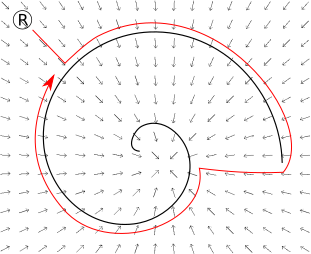
\includegraphics[width=\linewidth]{/home/ams/TinyRobo/docs/spiral_trap.png}
	\end{subfigure}
	\begin{subfigure}{0.45\textwidth}
		%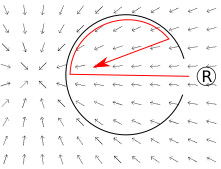
\includegraphics[width=\linewidth]{/home/ams/TinyRobo/docs/wall_follow_trap.png}
	\end{subfigure}
	\caption{Simple obstacles that result in looping behavior for a bug algorithm that combines wall following with leaving the obstacle when the vector field points away from the obstacle.}
	\label{traps_for_wall_follow}
\end{figure}

In none of these cases is the goal unreachable, in that it is a member of the same set of points as the open space of the environment, but attempts at obstacle avoidance preclude the robot reaching it. 

\section{Code Generation Refinement}

Rather than rejecting bug algorithms because they cannot be usefully combined with a global vector field, the vector field representation of the space was rejected. 
Vector fields have other problems, beyond unsatisfactory composition with complete motion control planners such as the bug algorithm family. 
A vector field cannot represent a path that crosses itself, such as a patrol route that is a loop.
In the continuous case, a vector field is represented by a function that maps all points in the space to a vector representing the desired robot heading at that point. 
However, because a function produces exactly one value, each point can only have one heading, while the intersection point of a path has two headings, at different points in time. 
For a vector field broken up into discrete grid cells, the same problem applies, but to regions rather than points. 

One potential solution to this problem with vector fields is to have multiple vector fields, or multiple values at each point, and allow the robot to maintain a program counter, which it uses to determine which field or which value to use at a given point. 
The counter is incremented on departure from a vector field grid cell, and then on return to that cell, the new value of the program counter is used in a guard, which results in the robot using the second value of the heading. 

For example, the GCPR statements:\\
(self.is\_in((1.745, 1.921), (1.245, 1.421)) and pc\_is(1), self.set\_desired\_heading(2.332), 0.9)\\
(self.is\_in((1.745, 1.921), (1.245, 1.421)) and pc\_is(2), self.set\_desired\_heading(1.031), 0.9)\\
will result in the robot using the heading 2.332 when it passes through the grid region if the program counter is 1, and 1.031 when it passes through the grid region with the program counter set to 2 (while, unfortunately, not defining a desired heading if the program counter is set to some other value).

Using a program counter to select possible headings for a discrete vector field grid cell has the drawback that the program counter must be incremented on leaving the cell, as incrementing it while remaining in the cell will cause a change of heading.
As a result, the generated program must have guards on all cells surrounding the cell, which increment the program counter when triggered. 

Further adding to this complexity is the problem of sensor noise. 
If sensor noise causes the robot to erroneously detect that it has entered the neighboring cell, then the program counter could be incremented without the robot actually leaving its current cell. 
On the next update of the noisy position sensor, the robot could then ``return'' to the current cell, and change direction due to the incorrectly implemented program counter. 

As a consequence of the complexity attendant on repairing the inability of the vector field to represent paths containing loops, the underlying representation of the conversion of user paths into robot programs was changed to avoid the use of vector fields. 

\subsection{Approaching a Point}

The basic action of the robot is to move from one location to another. 
Under the assumption that there exists some form of localization, which must hold in order to support the type of user interface described in this work, the simplest approach to navigation to a point is for the robot to rotate to face that point and then move forwards towards it. Once the point is reached, the robot should stop. 

Reaching of a point is more complex for swarm robots than it is for single robots. 
Some work assumes that robots in the abstract are points, and as they occupy no area, any number of them may congregate at a mathematical point. 
In the real world, while a point may be described precisely, it is usually sufficient to arrive within some small distance $\epsilon$ of it to say that the robot has reached the point. 
However, robots also take up space in the real world, and so as more and more members of the swarm arrive at the point, the later arrivals may be precluded from actually approaching to within $\epsilon$ of the point.
In this case, it is desirable to have a definition of arrival that expands to allow robots to approach the point as closely as they can and stop when that condition is met. 

For example, when a robot arrives at the point, it might stop, but broadcast a message to local robots that it is at the point. 
Robots arriving after the first would then navigate around it, keeping track of the minimum distance to the goal. 
After finishing a circumnavigation, the robot would then return to the closest point to the goal. 
As more robots arrive, the local minimum in the approach to the target point may become occupied by another robot, and so if that point is occupied, the robot would then have to perform another circumnavigation to find a new closest point. 
Because every iteration of this loop either occupies the closest point with a robot, or detects that the closest point has become occupied by another robot, and triggers another iteration, it will eventually position every robot as close as possible to the goal. 

\section{Completeness of Navigation}

Moving to a point is implemented as a bug algorithm. As described earlier, bug algorithms are complete, in that they navigate the robot to a point, or determine that the point cannot be reached. A review of eleven bug algorithms can be found in \citep{ng2007performance}. 

As stated earlier, it is preferable to have the robots follow the user-specified path, as following the user path is both more understandable to the user, and may allow the system to use information that the user has and the robot does not. 
A user path can be followed by a bug algorithm by breaking the user path into a series of points, and using a bug algorithm to navigate to each point in turn. 
Because the bug algorithm is complete, it can either reach the target point, or determine in finite time that the point is not reachable. 
For every point except the last in the user path, if the point is not reachable, the program can simply reset its target point to the next point along the path. 
Dropping points from consideration in this way will result in the robot deviating from the path, but the reason for the deviation is clearly explainable to the user, both from a program logic standpoint, and visually, as the interface displays the progress of the robot around the obstacle. 
If the last point of the user path is not reachable, the user-commanded path cannot be successfully completed, and so the user should be informed that the robot cannot reach it. 

Unfortunately, most of the bug algorithms have the requirement that the obstacles in the environment are not moving.
Indeed, the presence of moving obstacles results in navigation becoming undecidable without knowledge of the future movement of the obstacles, as an obstacle can move to occupy the robot's goal. 
Unless it is known whether the obstacle will move off the goal in the future, it cannot be determined whether the goal is unreachable, or just not currently reachable. 

The Tangent-bug algorithm has been extended to handle moving obstacles, given a number of constraints \citep{kamon1998tangentbug, tomita2009sensor}.
The main constraint that affects the use of this algorithm is that the obstacles are constrained to be moving at a velocity that is slower than that of the robot.
This constraint is required because if the robot is circumnavigating the obstacle, and the obstacle is moving faster than the robot, then in the time that the robot requires to circumnavigate the perimeter of the obstacle, the obstacle will have moved a distance greater than its own perimeter is long, and the circumnavigating robot will have moved with it.
As a consequence, the circumnavigating robot might not return to its own previous path and cross it, which is the condition that Tomita and Yamamoto use to determine that the robot should leave the obstacle. 

At first, this would appear to be a problem for swarm robots, because if the robots are the same, they will be moving at the same speed. 
If one moves in a straight line, and the other attempts to circumnavigate it, the circumnavigating robot will never cross its own path for the reason described above, and so never leave. 
However, if the robots are using the same bug algorithm, this trap will not be sprung, because each robot will attempt to circumnavigate the other. 
If they attempt to circumnavigate each other in opposite directions, they will spiral around each other, leading to at least one of the robots crossing its own previous path, and triggering the leave condition of the algorithm. 
If they attempt to circumnavigate each other in the same direction, they will come to a position side-by-side, as neither can outpace the other, but neither will pull away from the other because they are attempting to follow each other's perimeters. 
In this case, they are pointed towards the goal, because in the absence of an obstacle, Tomita and Yamamoto's modified Tangent-bug orients the robot towards the goal, and so before they encountered each other, the robots were oriented towards the goal.
The robots will then approach the goal, and one will arrive, while the other circumnavigates the first until it detects that it cannot arrive at the goal. 

Tomita and Yamamoto do not deal with the decidability of their modification of Tangent-bug because they constrain the goal point to be not within an obstacle, and so reachable by the robot. The original Tangent-bug will navigate the robot to the goal if it is reachable, or circumnavigate the obstacle, returning to its starting point, whereupon it detects that the point is unreachable \citep{kamon1998tangentbug}. Since Tomita and Yamamoto constrain the goal to not be within an obstacle, the original Tangent-bug will reach it. 

In the case of moving obstacles, if the goal is covered by an obstacle, the obstacle is either moving or not moving. If the obstacle is moving, the modified Tangent-bug will not return to its original hit point, which is either left behind or covered by the obstacle, but will eventually cross itself, and leave the object towards the goal.
If the obstacle is still covering the goal, this process will repeat until the object is not covering the goal anymore, and the robot will reach the goal. 

In the case of swarm robots, as described above, some mechanism may be needed to determine that the goal is occupied, possibly by other swarm members, and to stop at a location near the goal. 
The stopping condition of the original Tangent-bug in the case where the goal is unreachable extends naturally to swarm robots. 

If a robot is the first to arrive at the goal, the goal is not occupied, so the robot occupies it and stops. 
If a robot is not first to arrive at the goal, the goal is occupied by a robot, which is stopped. 
The new arrival treats the stopped robot as an obstacle, circumnavigates it, returns to the original hit point and so detects that the goal is unreachable, and stops. 
If multiple new arrivals get to the stopped robot(s) at the same time, the conditions above hold, and so they eventually either cross their own paths while trying to circumnavigate another robot that is also circumnavigating an obstacle, and so leave and return (and so become later arrivals), or complete a circumnavigation and return to their own starting point and stop (becoming part of the obstacle).

If a maximally dense cluster of robots is desired, the unreachability check of Tangent-bug can be extended. 
Once the goal is determined to be unreachable, the robot performs another circumnavigation of the blocking obstacle to find the closest point to the goal, and returns to that point. 
That point has either been occupied by another robot, in which case the robot repeats this step, or occupies that point if it is free. 
Because every iteration of this step fills the point closest to the goal with a robot, the cluster of robots is packed as close to the goal as possible. 

 \begin{figure}
 	\centering
 	\digraph[scale=0.6]{TangentBugMod}{
 		
 		start -> obstacleToGoal;
 		obstacleToGoal -> aimToGoal [label="No"];
 		aimToGoal -> atGoal;
 		atGoal -> stop [label="Yes"]; 
 		atGoal -> obstacleToGoal [label="No"];
 		obstacleToGoal -> recordHit  [label="Yes"];
 		recordHit -> followEdge;
 		followEdge -> closerPoint;
 		closerPoint -> leaveObstacle [label="Yes"];
 		leaveObstacle -> obstacleToGoal;
 		closerPoint -> pathCross [label="No"];
 		pathCross -> returnToHit [label="No", color="blue"];
 		returnToHit -> followEdge [label="No", color="blue"];
 		returnToHit -> unreachable [label="Yes", color="blue"];
 		unreachable -> lastPoint [color="blue"];
 		lastPoint -> updateGoal  [label="No", color="blue"];
 		lastPoint -> stop  [label="Yes", color="blue"];
 		updateGoal -> obstacleToGoal [color="blue"];
 		pathCross -> obstacleToGoal3 [label="Yes"];		
		obstacleToGoal3 -> followEdge2 [label="Yes"];		
		obstacleToGoal3 -> aimToGoal[label="No"];		
		followEdge2 -> obstacleToGoal3;
		
 		obstacleToGoal [label="Obstacle in direction of goal?"];
 		aimToGoal [label="Orient towards and move to goal"];
 		atGoal [label="At goal?"];
 		leaveObstacle[label="Leave obstacle"];
 		recordHit [label="Record hit point"];
 		unreachable [label="Goal is unreachable", color="blue"];
 		updateGoal [label="Next point is new goal", color="blue"];
 		lastPoint [label="Is this the last point?", color="blue"];
 		followEdge [label="Follow obstacle edge"];
 		returnToHit [label="Returned to hit point?", color="blue"];
 		closerPoint [label="Closer to goal than hit point?"];
 		pathCross [label="Crossed own path?"];
 		obstacleToGoal3 [label="Obstacle in direction of goal?"];
 		followEdge2 [label="Follow obstacle edge"];
 	}
 	\caption{The proposed modifications (in blue) to the Tomita and Yamamoto Tangent-bug algorithm for user path following in cases with multiple robots, some of which may be treated as moving obstacles. This flow chart does not include the option for maximally dense packing at the goal described in the text. }
 \end{figure}

\chapter{Compiler Verification}

The design of a compiler which verifies that its output is correct What does it mean for a program to be correct? Free from things like assignment of variables to the wrong type, buffer overflows, off-by-one errors, etc. Does not mean that the program does what the programmer intended, just that it does whatever it does without errors. 
Correctness is judged with respect to a specification. 
Partial correctness - if an answer is returned, it is correct. 
Total correctness - requires that program is partially correct and terminates
No general solution to halting problem, needs specific proof per-program
Compiler correctness shows that a compiler behaves according to its specification
I don't currently have a language specification for the gesture language 

One method of testing compilers is the operation of a fuzzer \citep{miller1990empirical}. A fuzzer, in the general case, generates input for programs that, while technically legitimate input, causes unexpected behavior such as program crashes. A fuzzer for compilers uses a description of the source language to generate programs that are considered valid under the description, and then attempts to compile them using the compiler. It can also attempt to generate programs that are deliberately incorrect, to test the ability of the compiler to accurately report errors, and to ensure that the compiler accepts all correct programs and no incorrect programs, as in \citep{bazzichi1982automatic}. 
Because the internal structure of the compiler is not known, a generator cannot be certain that it causes all code paths in the compiler to be executed, but it can be certain that the generated test programs use all of the syntactical elements of the language, since all of the elements are described in the language specification. Interestingly, Bazzichi and Spadafora's work predates the use of the term ``fuzzer'' by 8 years, but clearly describes the same process.

Translation validation \citep{pnueli1998translation}
verifies compiled code against input code rather than attempting to verify that a compiler correctly translates all input programs.
Verifies that the compiler correctly transforms a specific input program. 
Needs:
 - A common semantic framework for the representation of the source code and the generated target code (probablistic finite automaton?)
 - A formal description of "correct implementation"
 - A proof method for verifying that one instance of the semantic framework (the output) correctly implements another one (the input)
How is the IR not the common semantic framework?
%
 




% !TeX root = ams_thesis.tex
\chapter{Program Translation Implementation}

At the outset of this work, it had been hoped that there existed some form of transformation from the language defined by creating a formal description of an unambiguous subset of the user gestures to a potential language of robot behaviors. 
While the language of robot behaviors is itself not terribly well-defined, approaches such as the flavors of AutoMoDe and Supervisory Control Theory hint that the output language would likely be able to be represented as a DFA or PA, and so the resulting programs could then be amenable to analysis using e.g. PRISM \citep{KNP11}.

However, the user gesture language as defined by this work is actually quite vague, when it comes to allowing a robot to perform the expected actions. 
Users were told to assume that the system was capable of understanding their orders, so they merely had to indicate what they wanted the system to do, and it would then do it. 
Alan Perlis has been quoted as saying ``When someone says `I want a programming language in which I need only say what I wish done,' give him a lollipop.'' \citep{PerlisYaleLolz}.  
Such systems are substantially more difficult than the recipients of lollipops expect, because they rely on a large amount of \emph{a priori} information shared between the person issuing the command, and the system executing it. 

For example, in the box-moving task, the users would frequently move the robots to surround the box, and then move the robots to the goal area. 
However, one might expect that robot control programs would attempt to avoid obstacles, and so would just go around a box. 
Without the knowledge that boxes are acceptable to push against, no motion would occur, and the robots would in fact actively resist being steered to push the box. 
Even this knowledge shows the limitations of the gesture as a way of conveying a program to a robot.
The user data set does not have clear gestures for conveying that box-pushing is desirable, how to recognize the presence of a box, how to tell one box from potential other boxes, or how to convey that any particular object can be pushed, rather than just boxes. 
Instead, users seemed to assume that the robots understood, as the user did, that the box was a thing that could be moved, and so did not have to be told.

Because the user gestures did not convey all of the information required to perform tasks, there is not a transformation that could operate purely on the user input to produce a program as output. 
Instead, the output program also has to include elements of planning and other knowledge. 
Because the system was intended to operate in a potentially unknown environment, the bug, dispersion, and occlusion-based transportation algorithms discussed in the previous section were used. 
If the environment were known, or communication were assumed to be reliable, other algorithms could be used. 
Indeed, the translation layer could be modified to switch algorithms based on the parameters of the swarm it is creating programs for and their environment. 

The development of the translation layer was performed in a manner similar to a compiler, which permitted the planning and other algorithms to be built into output programs by the translation layer. 
The input language was the user gestures, including which robots were selected and which user-specified paths were created. 
These inputs were used to parameterize the chosen algorithms, and the robots selected were used to determine the distribution of the resulting programs.
As a result, this work does not end up breaking away from iterative hand-coding, it just moves it from being done as a way of controlling the swarm, to being done as part of the creation of the control interface. 
For the motivating example from the introduction, urban search and rescue, this is acceptable, as it does not require the end user to program the swarm. 
It is also somewhat risky, as the resulting system may not have the flexibility that end users require. 

\section{Implementation Details}

User gestures arriving at the translation layer are stored in a stack until an end-of-command gesture arrives. 
The gesture sequence is then translated into a program that is parsed by the Lark parser library. 
Lark is an Earley parser, and so can parse all context-free grammars, although the current gesture language is not sufficiently complex to actually need this level of power. 
The resulting parse tree is then walked to generate GCPR programs that implement the algorithms described in chapter \ref{chapter:Implementation_of_Swarm_Actions}.

Basic movement to points is implemented using the variant of tangent bug. 
Path following and formation combines the basic movement to points with a sequence of GCPR instructions that implement a program counter, and set the goal based on the program counter. 
As each point is either reached or determined to be unreachable, the goal is advanced to the next point.
For motion along paths, the goals are set to points along the path, ending at the final goal. 
Formation allows the robot to stop at reachable points on the formation, but not unreachable points.  

Patrol also uses modified tangent bug, but instead of terminating when the program counter, and so the goal, reach the final position, the program counter and goal are reset to the start point of the patrol.  
As a consequence, the resulting program intentionally contains an infinite loop, but it can be interrupted by assigning a new program to the swarm. 

Dispersion is implemented using a minimalistic range sensor. 
Each robot can detect if there are other robots within a fixed range. 
If there are more than two robots in the range, the robot moves forward, avoiding obstacles. 
If there are exactly two robots in range, the robot stops. If there are less than two robots in range, the robot executes a U-turn and drives in a straight line, avoiding obstacles, until one of the other situations occurs. 
This algorithm is a GCPR implementation of the $\alpha$-algorithm of Winfield \emph{et al.}, and so shares its strengths and weaknesses  \citep{winfield2008modelling}.
Notably, the algorithm is not certain to prevent the separation of the swarm into subswarms that are not connected. 
More sophisticated programs, possibly using more communication, can prevent these issues, but since the requirement of the behavior is that the robots disperse, rather than that they maintain a particular level of network connectivity, there is no need for this particular implementation to enforce connectivity. 
Indeed, simply moving the robots to random locations uniformly selected would ``disperse'' them. 
However, selecting points would require foreknowledge of the area to disperse into. 
The $\alpha$-algorithm was chosen instead because it can operate in a previously unknown area, and because the resulting distribution looks even, visually. 
A randomly selected set of points from a uniform distribution may place two robots right next to each other, which, while ``uniform'' in a statistical sense, would appear uneven to the user, and not satisfy their intuitive understanding of dispersion. 
If dispersion in swarm robots continues to be a problem of interest, it is likely worth investigating the tradeoffs between speed of convergence, quality of dispersion, and user satisfaction with various methods. 

Manipulation was implemented as a simple version of occlusion-directed transport. 
If the robot is not near the target object, it attempts to move to the target object while avoiding obstacles, using the modified tangent bug algorithm. 
When the tangent-bug algorithm detects that the goal is unreachable, because it is inside of the mobile object, the program switches to occlusion-based manipulation. 
The robot wall-follows around the object until a line from the robot to the goal intersects the object, and then pushes in that direction. 
While in this mode, the robot continually updates the direction of the goal, and switches between getting in position and pushing the object, as needed. 
As with the original occlusion-based manipulation, this algorithm is ignorant of obstacles on the opposite side of the object from the robot, and so can get stuck. 
However, as the system can accept a path for the object to be pushed on, the user can attempt to specify a clear path for the robots to move the object along. 

%\chapter{Compiler Verification}
%
%The design of a compiler which verifies that its output is correct What does it mean for a program to be correct? Free from things like assignment of variables to the wrong type, buffer overflows, off-by-one errors, etc. Does not mean that the program does what the programmer intended, just that it does whatever it does without errors. 
%Correctness is judged with respect to a specification. 
%Partial correctness - if an answer is returned, it is correct. 
%Total correctness - requires that program is partially correct and terminates
%No general solution to halting problem, needs specific proof per-program
%Compiler correctness shows that a compiler behaves according to its specification
%I don't currently have a language specification for the gesture language 
%
%One method of testing compilers is the operation of a fuzzer \citep{miller1990empirical}. A fuzzer, in the general case, generates input for programs that, while technically legitimate input, causes unexpected behavior such as program crashes. A fuzzer for compilers uses a description of the source language to generate programs that are considered valid under the description, and then attempts to compile them using the compiler. It can also attempt to generate programs that are deliberately incorrect, to test the ability of the compiler to accurately report errors, and to ensure that the compiler accepts all correct programs and no incorrect programs, as in \citep{bazzichi1982automatic}. 
%Because the internal structure of the compiler is not known, a generator cannot be certain that it causes all code paths in the compiler to be executed, but it can be certain that the generated test programs use all of the syntactical elements of the language, since all of the elements are described in the language specification. Interestingly, Bazzichi and Spadafora's work predates the use of the term ``fuzzer'' by 8 years, but clearly describes the same process.
%
%Translation validation \citep{pnueli1998translation}
%verifies compiled code against input code rather than attempting to verify that a compiler correctly translates all input programs.
%Verifies that the compiler correctly transforms a specific input program. 
%Needs:
% - A common semantic framework for the representation of the source code and the generated target code (probablistic finite automaton?)
% - A formal description of "correct implementation"
% - A proof method for verifying that one instance of the semantic framework (the output) correctly implements another one (the input)
%How is the IR not the common semantic framework?
%
%\section{Limitations}
%
%input semantics don't include way for user to set robot heading, might be useful for sensor overwatch






% !TeX root = ams_thesis.tex
\chapter{Contributions} \label{chapter:Contributions}
\thispagestyle{fancy}

\section{Swarm Hardware and Software Platform}

A hardware platform for control of small, inexpensive swarm robots was developed. 
The fact that swarm hardware across the literature has roughly the same general layout for the hardware can be viewed as an example of similar needs leading to similar solutions.
Gianpiero \emph{et al.} describe a reference model that is inspired by the E-puck \citep{francesca2014automode}.
The reference model could probably generalize well to other hardware, as the E-puck it is based on also has a ring of IR sensors and differential drive. 
The GRITSbots, Amir, and Colias all have a ring of IR sensors, as do many other designs. 
Most swarm robots use differential drive for steering, through either a sealed gearbox or direct drive.
A generalized reference model would also be useful for developing SCT generators for robot control, as the set of free behavior models is specific to the robot, and so could be reused for new tasks using the reference system. 

TinyRobo aimed to drive the cost of this style of robot down further, by virtualizing the sensors. 
The TinyRobo ROS modules include the ability to have configurable virtual laser scanners, range and bearing sensors for inter-robot sensing, and virtual networks, all of which can be easily customized to allow experimentation with sensor noise or failure. 

The use of children's toys as a mobility platform does not result in substantial savings, or even in easier assembly of the platform. 
Toys also have reliability problems that offset their possible utility as mobility platforms. 
However, if some other drivetrain is used, the power and control module is still cheap, small, and easy to use. During the course of this work, 3D printers have dropped substantially in price, so the difficulty of producing custom small mechanical assemblies has been significantly reduced since the time of the development of e.g. the Jasmine micro-robots. 
As a consequence, the use of a 3D printed robot chassis and the TinyRobo control modules can produce a very inexpensive swarm platform. 

%Assuming the toys are replaced with either stepper motors or small DC motors with built-in gearboxes, the complete hardware platform is similar to Colias or the GRITSbots.
%A review of online suppliers at the time of this writing indicates that small stepper motors designed for use in cameras area available for well under one dollar per unit, so this change would actually result in substantial cost savings. 
%However, it would require alteration of the drive electronics to control a stepper motor. 
%Small DC motors with sealed gearboxes are available for \$3-5 in single quantities as well, so combining them with a 3D printed enclosure would likely yield a more reliable base, at a similar price to the toys used in this work. 
Resolving the problems with that this work ran into with AprilTags would result in an approach closer to mROBerTO.
The motor drive electronics would remain the same, but either fixed color tags or LEDs as identity indicators would be used to track the robots. 
It has been suggested that a ring of addressable LEDs could be used to convey information from the swarm to the control system, by changing the color of LEDs on the ring or animating them in patterns. 
Since such a display could also be meaningful to the user, this may be an interesting direction for future research in HSI for co-located swarms.  

Because of the modular nature of the system, the ROS stack can be interfaced with simulations as well as with real robots. 
The main feature making this possible is the fact that the communication with the swarm hardware operates using standard ROS modules as much as possible, and only performs hardware-specific operations where they cannot be avoided. 
This flexibility enabled an easy transition to testing in simulation when it became apparent that the toy bases were not going to become a useful platform. 

\section{Multitouch Gesture set for Swarm Control} \label{section:Multitouch_Gesture_set_for_Swarm_Control}

Gestures were collected from 50 users to define a gesture set for multitouch swarm control. 
Analysis of the data showed that there were variations in the uses of certain gestures as the size of the swarm increased. 
In particular, the use of selection gestures increased in the 10 and 100 robot cases, but dropped off for the 1000 robot swarm. 
Tap gestures were more likely to be used for selection in the unknown, 1, and 10 robot cases than the other cases, while group selections were used mainly in the 10 and 100 robot cases, and less in the 1000 robot case. 
The 10 robot case seems to be the transition point where use of group or single tap selections are equally used. 

Showing the area occupied by the swarm as a cloud had very similar use of selections to the one robot case. 
Box selection was never used, lasso was used rarely, and tap selections were the most common selection gesture by far. 
These changes to the user's choices of gesture support the hypothesis that the gesture selection does change with the user's perception of the swarm, both the visible number of robots and whether the swarm is rendered as individual robots or a coverage area. 

There is evidence from the user survey and gesture selection that video games and other prior experiences with multi-touch interaction devices have an influence on the gestures used. 
The interface design used in the experiment was initially somewhat like the interface of a realtime strategy game, and as a result, seems to have cued users who had played realtime strategy games (RTSs) to use styles of interaction common to RTSs.
Designers of future interfaces can interpret this as both a strategy and a warning. 
As a strategy, interfaces can be designed specifically to include design features from games, and so cue the users that the interface supports the interactions that are common in the genre of game that the interface emulates. 
However, it can also be a warning that if an interface resembles a game, the users will expect those interaction styles, and may entirely avoid other interaction styles that do not fit with their expectations. 
The total absence of pinch gestures on the part of RTS gaming users is such a missing interaction. 
At a more abstract level, designers would be wise to avoid leaning too heavily on game-based cues in user interface design, unless they are certain that their users are gamers, or the cue will be missed. 

Despite being told that the device is multitouch, most users made very few two-handed gestures, although half of the users made at least one two-handed gesture.  
Voice commands were more common in the data set collected for this experiment than in previous experiments that allowed users free reign in choice of their command set. 
It is speculated that this is due to the rise in functionality and prevalence of ``voice assistant'' technologies in smartphones and home appliances such as Google Home. 
This transition would be similar to the transition observed in previous work, where people who had smartphones used pinch gestures far more than people who did not have experience with smartphones or similar multitouch devices. 

It had been surmised that one possible sign that the user was treating the robots as a group would be that some parts of the group would be neglected. 
This generally did not occur. 
Instead, the users used selection gestures that included all robots, and when asked about inclusion in gestures, erred on the side of including more robots. 

There were also relatively few gestures treating the robots as a deformable mass that could be pushed around, like a pile of sand or other small objects. 
Physical affordances like this were speculated to be more likely, given the direct interaction style of the multitouch screen. 
Their absence could be viewed as highlighting the users' understanding of the screen as an image, and so not something that supports physically-afforded interactions. 

In future, it would be interesting to repeat this work with a condition that does not display the robots in the user interface at all. 
It is expected that for conditions such as the ``move the crate'' tasks, the user would simply indicate the crate should move to area A, without concern for which robots perform the moving. 
However, such an interface would not afford indicating particular robots or groups, so tasks such as dividing the robots around an obstacle may become impossible to perform. 

\section{Compilation of User Gestures into Robot Programs} \label{section:Compilation_of_User_Gestures_into_Robot_Programs}

This project shows a basic conversion from user gestures into a set of command programs to be distributed to the swarm robots.
These command programs are intended to balance desirable formal properties of the programs, such as convergence within bounded time, use of local-only sensing, and completeness, with reflecting the user's intentions in the observable behavior of the swarm. 

In attempting to derive complete program frameworks for the tasks specified in the user studies, it was determined that complete controllers for some simple tasks may not exist. 
For example, while it is possible to have a complete controller for motion to a point, it is impossible to have a complete dispersion controller that relies on only local sensing. 
In cases where completeness could not be determined, or was determined to be impossible, the controllers used are developed to use local-only sensing and if they fail, to do so in a manner that is intelligible to the user. 

The translation between user commands and robot programs in this work was developed using a method similar to compiler development, where an input language was defined from the user gesture commands, and an interpreter was developed to take strings in the language of gestures, and output control programs in as statements in an implementation of guarded control programming with rates (GCPR) \citep{napp2011compositional}.  
Previous work in gesture control for small groups of robots was also able to recognize a grammar of user inputs using a finite state machine \citep{micire2010multi}.
It had been initially hoped that there would be a universal abstraction or transformation that could represent the conversion of all gestures into all robot commands representing those gestures, rather than having different sets of behaviors, with different properties, which could be constructed from the user gestures after recognizing those gestures. 
However, user gestures do not provide a sufficiently explicit means of designing a program in realtime to allow for the full automation of the generation of control programs without assuming an amount of \emph{a priori} knowledge that is unrealistic in practice. 
For example, while there is a gesture for disperse, the gesture itself does not contain information about how the dispersion should be performed. 
Similarly, while the gestures used to indicate that an object should be moved to a location contain information about what the movement should be, they do not contain information about how the movement should be accomplished. 
Because these elements are not present in the user input, any universal transformation that has them in its output would have to essentially make them up. 
As a consequence, the translation was implemented in the way that programming languages are usually implemented, with a developer supplying the method that the robots would use to fulfill the user's commands. 

There are a number of threads in current swarm robotic research that may eventually permit the engineering of swarm behavior from high level descriptions, many of which are discussed in Section \ref{section:Swarm_Software_Development_Methods}. 
One that is not discussed in great depth there is the field of attempts to find mappings between relatively low-dimensioned swarm macrostates and potentially extremely high-dimensional state spaces representing each robot individually. 
While some work has been done in controlling swarms with controllers operating on macro-level behavior, such as attractors, there is not yet an engineering discipline that would guide the creation of arbitrary swarm behaviors under real-world complexity \citep{brown2014human}. 
As this area of swarm robotics develops, user interfaces will have to develop with it, in order to allow humans to operate these systems in a fluent manner. 



\bibliography{../proposal/swarm.bib}
%\bibliographystyle{apalike}

\begin{appendices}
\chapter{Coding Definitions for User Gestures}

\section{General Points} \label{section:General_Points}

Code the time that the user ends the gesture (takes their finger off the screen), to at least 0.1 second, 0.01 second is better. 
 
Code all interactions with the screen. Some users draw on the screen with their finger while explaining their commands, or describing the reaction they would expect from the system. These should be coded because 
\begin{itemize}
	\item The system, being a dumb computer, can't determine the user's intentions
	\item Everyone coding the same things helps with inter-coder reliability 
\end{itemize}

Use the ``example'' flag when coding these actions. The example flag is also used for if the user repeats their command while describing it, but not for the first time they do it. 
\begin{itemize}
	\item Do not code non-contact examples, which is to say when the user is discussing their thinking and not touching the screen, even if they are repeating an action that they did while touching the screen. Only count examples that touch the screen. 
\end{itemize}
 
Lasso and Box Select are essentially specific forms of Drag, but the users frequently clarify these actions by saying things like ``I'd take these robots'' or ``Select some robots...'', or by mentioning their inspiration for the action, such as Real Time Strategy (RTS) games or selecting multiple files on the desktop. Users are generally consistent, so if a user has used Box Select or Lasso previously with a clear statement of their intent, future Box Selections or Lassos can be coded as such without requiring the user to say what they're doing. 
 
Generally, if the user does the same action with both hands, and the actions have the same object, such as dragging the robots to one point with both hands, it's a single action, but coded as 2-handed. If the actions have different objects, such as dragging one group of robots with one hand and a different group with the other hand, it's two drag actions, although they may have very similar or the same ending time. 

\section{Gestures} \label{section:Gestures}

Drag - User places their finger or fingers down and moves them to a different location while touching the screen. The drag ends when the user lifts their finger, so drawing a circle around robots and then to another location is a single drag action, not a lasso followed by a drag. 
\begin{itemize}
	\item If two or more drags are performed at the same time on the same object, code it as one instance of two-handed drag, not two instances of drag. 
	\item If two or more drags are performed at the same time, but have different objects, code it as two drags with different objects.
	\item If the user is drawing a specific form, use the ``draw'' flag of the drag code, and describe what they drew. 
	\item If a user lifts their finger while drawing something in multiple parts, such as writing out words, or drawing arrowheads on lines, code each time they lift their finger as a separate drag. 
	\item A person dragging the side of their finger is an ``other'', not a ``drag''
\end{itemize}

UI - User interacts with the screen while describing a UI element such as a menu, drop-down box, on-screen joystick, or similar. Also used for description of a sequence of events, such as the user saying ``I would pull up a menu'' or ``I would type in a command''. 
\begin{itemize}
	\item Do not code the user describing something that they would like to have in the UI unless they are describing how they would use it to issue commands for the current task. 
	\item If the user taps for a menu, or drags a menu down, code it as UI, not as a tap or drag. \item Code UI actions at the end of the action, not at the end of the user description. 
	\item If the user taps the same button many times, code each time (don't combine them)
\end{itemize}
 
Tap - User places finger on screen and lifts it immediately, without moving it a significant distance. Taps longer than one second are ``Holds'', as defined below. 
 
Double-tap - User taps twice with both taps falling within an inch of each other and within one second, and without describing tapping on something else, such as tapping to bring up a menu and then tapping something on that menu. 
\begin{itemize}
	\item Taps for actions such as drawing a dotted line should be coded as individual taps. 
Double-taps are coded as taps with the -c (for ``count'') flag set to 2. 
\end{itemize}

Triple-tap - As with double-tap, but with three taps. 
\begin{itemize}
	\item Anything beyond three taps should be coded as individual taps, but obviously with close-together time codes. Quadruple-taps and beyond are also comparatively rare. 
	\item Triple-taps are coded as taps with the -c (for ``count'') flag set to 3. 
\end{itemize}

Hold - User places one finger on the screen and leaves it there without moving for more than one second. Code the time at the end of the hold, when they lift their finger. 
\begin{itemize}
	\item Holds are coded as taps with the -h (for ``hold'') flag. 
\end{itemize}

Pinch - User places two fingers on the screen, resulting in two points of contact, and moves them towards each other in a line. 
\begin{itemize}
	\item The Pinch code has flags for specifying the number of fingers and hands used, please code them appropriately.
	\item Multiple pinches at the same time on the same object should be coded as a single pinch instance. For a case where a user makes a pinch gesture with both hands at once, code it as a single pinch, with two hands and four fingers. 
	\item Multiple pinches at the same time on different objects should be coded as separate pinches, with the -o/object flag describing which things were pinched. 
\end{itemize}

Reverse pinch - User places two fingers on the screen, resulting in two points of contact, and moves them away from each other in a line. 
\begin{itemize}
	\item The Pinch code has flags for specifying the number of fingers and hands used, please code them appropriately.
\end{itemize}

Lasso - User touches on or near the robots and moves their finger in a closed shape (usually a circle or oval) around or over some set of the robots. Immediately precedes issuing some other command to the selected group. 
\begin{itemize}
	\item If it is unclear whether the user intended to perform this action as a selection, code it as a drag. 
\end{itemize}

Box select - User touches on or near the robots and drags their finger diagonally across the robots in a straight line, then lifts their finger. Immediately precedes issuing some other command to the selected group. 
\begin{itemize}
	\item If it is unclear whether the user intended to perform this action as a selection, code it as a drag.  
\end{itemize}

Voice command - Statements addressed to the robots, such as ``Robots, go to area A'', or statements such as ``I would tell the robots to form a square''. Code the time of voice commands at the end of the user's full sentence. 
\begin{itemize}
	\item If the user says something like ``Robots, do X and then do Y'', that's one voice command, don't break it into two commands at the ``and then''. 
\end{itemize}

Other - Anything not listed above, but intended by the user as a command for the robot. This code has a description field in the coding program, please use it to describe the action. 
\begin{itemize}
	\item Gestures over the screen, without contact, and that don't match the any of the other commands should generally be coded as ``Other'', but only if they are clearly intended as a command to the robot, not e.g. pointing at something on the screen or indicating the screen itself. 
\end{itemize}

\chapter{All Task Slides}

\section{1 Robot Case}

\begin{minipage}{\linewidth}
	\centering
	\begin{minipage}{0.42\linewidth}
		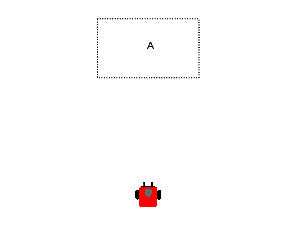
\includegraphics[width=\linewidth]{../ui_experiment/slide_images/Swarm_Robot_Control_-_Single_Robot_0003.png}
		\captionof{figure}{Move to A}\label{fig:sub1}
	\end{minipage}
	\begin{minipage}{0.42\linewidth}
		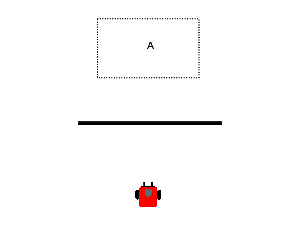
\includegraphics[width=\linewidth]{../ui_experiment/slide_images/Swarm_Robot_Control_-_Single_Robot_0005.png}
		\captionof{figure}{Move to A with wall}\label{fig:sub2}
	\end{minipage}
\end{minipage}

\begin{minipage}{\linewidth}
	\centering
	\begin{minipage}{0.42\linewidth}
		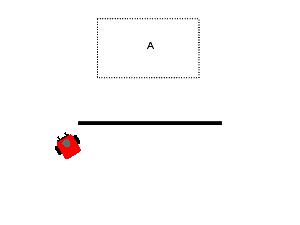
\includegraphics[width=\linewidth]{../ui_experiment/slide_images/Swarm_Robot_Control_-_Single_Robot_0007.png}
		\captionof{figure}{Stop the robot}
		\label{fig:sub1}
	\end{minipage}
	\begin{minipage}{0.42\linewidth}
		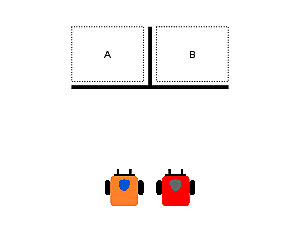
\includegraphics[width=\linewidth]{../ui_experiment/slide_images/Swarm_Robot_Control_-_Single_Robot_0009.png}
		\captionof{figure}{Orange to B, Red to A}
		\label{fig:sub2}
	\end{minipage}
\end{minipage}

\begin{minipage}{\linewidth}
	\centering
	\begin{minipage}{0.42\linewidth}
		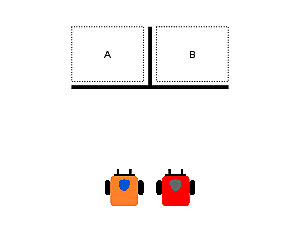
\includegraphics[width=\linewidth]{../ui_experiment/slide_images/Swarm_Robot_Control_-_Single_Robot_0011.png}
		\captionof{figure}{Orange to A, Red to B}
		\label{fig:sub1}
	\end{minipage}
	\begin{minipage}{0.42\linewidth}
		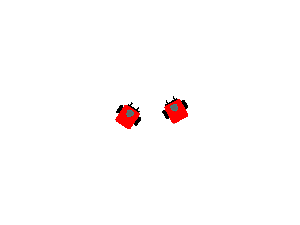
\includegraphics[width=\linewidth]{../ui_experiment/slide_images/Swarm_Robot_Control_-_Single_Robot_0013.png}
		\captionof{figure}{Divide group}
		\label{fig:sub2}
	\end{minipage}
\end{minipage}

\begin{minipage}{\linewidth}
	\centering
	\begin{minipage}{0.42\linewidth}
		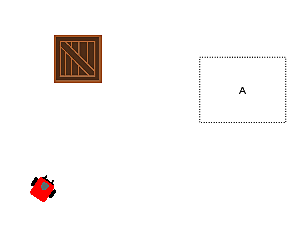
\includegraphics[width=\linewidth]{../ui_experiment/slide_images/Swarm_Robot_Control_-_Single_Robot_0015.png}
		\captionof{figure}{Move the crate to A}
		\label{fig:sub1}
	\end{minipage}
	\begin{minipage}{0.42\linewidth}
		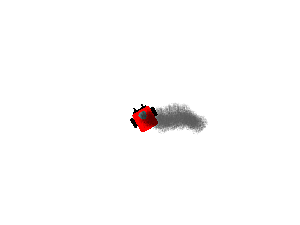
\includegraphics[width=\linewidth]{../ui_experiment/slide_images/Swarm_Robot_Control_-_Single_Robot_0017.png}
		\captionof{figure}{Mark defective robot}
		\label{fig:sub2}
	\end{minipage}
	\label{fig:single_robot_slides}
\end{minipage}


\begin{minipage}{\linewidth}
	\centering
	\begin{minipage}{0.42\linewidth}
		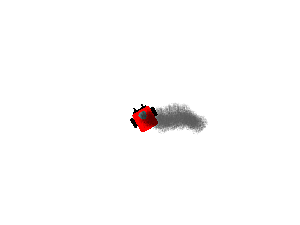
\includegraphics[width=\linewidth]{../ui_experiment/slide_images/Swarm_Robot_Control_-_Single_Robot_0019.png}
		\captionof{figure}{Remove defective robot}
		\label{fig:sub1}
	\end{minipage}
	\begin{minipage}{0.42\linewidth}
		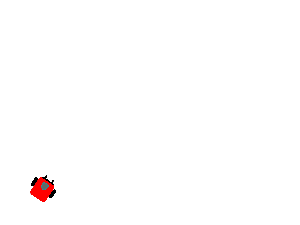
\includegraphics[width=\linewidth]{../ui_experiment/slide_images/Swarm_Robot_Control_-_Single_Robot_0021.png}
		\captionof{figure}{Patrol the screen border}
		\label{fig:sub2}
	\end{minipage}
\end{minipage}

\begin{minipage}{\linewidth}
	\centering
	\begin{minipage}{0.42\linewidth}
		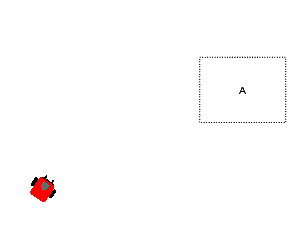
\includegraphics[width=\linewidth]{../ui_experiment/slide_images/Swarm_Robot_Control_-_Single_Robot_0023.png}
		\captionof{figure}{Patrol area A}
		\label{fig:sub1}
	\end{minipage}
	\label{fig:single_robot_slides_pt2}
\end{minipage}


\section{10 Robot Case}

\begin{minipage}{\linewidth}
	\centering
	\begin{minipage}{0.42\linewidth}
		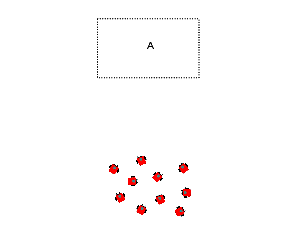
\includegraphics[width=\linewidth]{../ui_experiment/slide_images/Swarm_Robot_Control_-_10_Robot_0003.png}
		\captionof{figure}{Move to A}
		\label{fig:sub1}
	\end{minipage}
	\begin{minipage}{0.42\linewidth}
		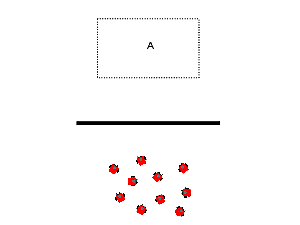
\includegraphics[width=\linewidth]{../ui_experiment/slide_images/Swarm_Robot_Control_-_10_Robot_0005.png}
		\captionof{figure}{Move to A with wall}
		\label{fig:sub2}
	\end{minipage}
\end{minipage}

\begin{minipage}{\linewidth}
	\centering
	\begin{minipage}{0.42\linewidth}
		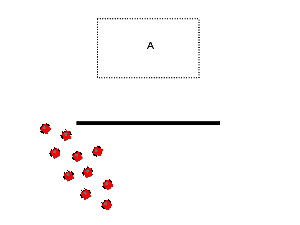
\includegraphics[width=\linewidth]{../ui_experiment/slide_images/Swarm_Robot_Control_-_10_Robot_0007.png}
		\captionof{figure}{Stop the robots}
		\label{fig:sub1}
	\end{minipage}
	\begin{minipage}{0.42\linewidth}
		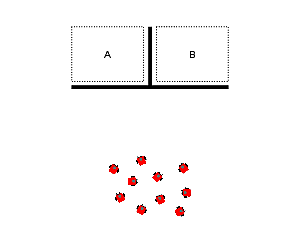
\includegraphics[width=\linewidth]{../ui_experiment/slide_images/Swarm_Robot_Control_-_10_Robot_0009.png}
		\captionof{figure}{Divide around obstacle}
		\label{fig:sub2}
	\end{minipage}
\end{minipage}

\begin{minipage}{\linewidth}
	\centering
	\begin{minipage}{0.42\linewidth}
		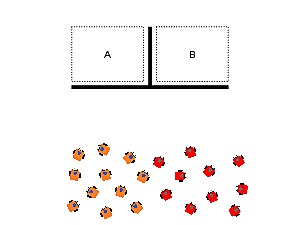
\includegraphics[width=\linewidth]{../ui_experiment/slide_images/Swarm_Robot_Control_-_10_Robot_0011.png}
		\captionof{figure}{Orange to B, Red to A}
		\label{fig:sub1}
	\end{minipage}
	\begin{minipage}{0.42\linewidth}
		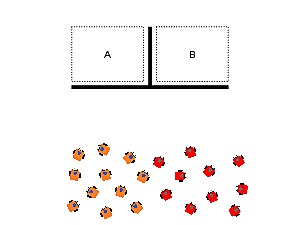
\includegraphics[width=\linewidth]{../ui_experiment/slide_images/Swarm_Robot_Control_-_10_Robot_0013.png}
		\captionof{figure}{Orange to A, Red to B}
		\label{fig:sub2}
	\end{minipage}
\end{minipage}

\begin{minipage}{\linewidth}
	\centering
	\begin{minipage}{0.42\linewidth}
		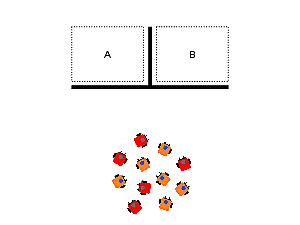
\includegraphics[width=\linewidth]{../ui_experiment/slide_images/Swarm_Robot_Control_-_10_Robot_0015.png}
		\captionof{figure}{Orange to A, Red to B}
		\label{fig:sub1}
	\end{minipage}
	\begin{minipage}{0.42\linewidth}
		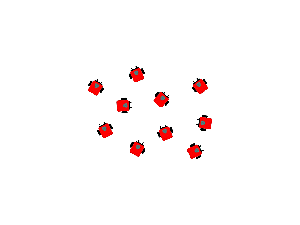
\includegraphics[width=\linewidth]{../ui_experiment/slide_images/Swarm_Robot_Control_-_10_Robot_0017.png}
		\captionof{figure}{Divide group}
		\label{fig:sub2}
	\end{minipage}
\end{minipage}
	
	
\begin{minipage}{\linewidth}
	\centering		
	\begin{minipage}{0.42\linewidth}
		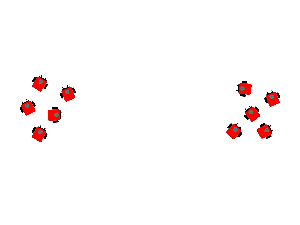
\includegraphics[width=\linewidth]{../ui_experiment/slide_images/Swarm_Robot_Control_-_10_Robot_0019.png}
		\captionof{figure}{Combine groups}
		\label{fig:sub1}
	\end{minipage}
	\begin{minipage}{0.42\linewidth}
		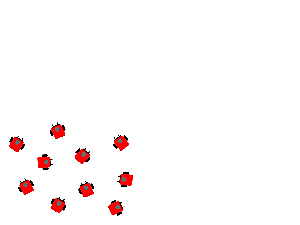
\includegraphics[width=\linewidth]{../ui_experiment/slide_images/Swarm_Robot_Control_-_10_Robot_0021.png}
		\captionof{figure}{}
		\label{fig:sub2}
	\end{minipage}
\end{minipage}

\begin{minipage}{\linewidth}
	\centering
	\begin{minipage}{0.42\linewidth}
		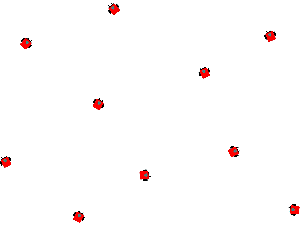
\includegraphics[width=\linewidth]{../ui_experiment/slide_images/Swarm_Robot_Control_-_10_Robot_0023.png}
		\captionof{figure}{}
		\label{fig:sub1}
	\end{minipage}
	\begin{minipage}{0.42\linewidth}
		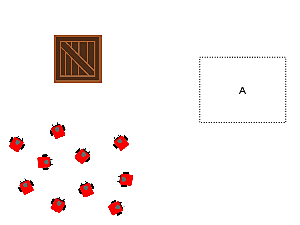
\includegraphics[width=\linewidth]{../ui_experiment/slide_images/Swarm_Robot_Control_-_10_Robot_0025.png}
		\captionof{figure}{Orange to A, Red to B}
		\label{fig:sub1}
	\end{minipage}
\end{minipage}

\begin{minipage}{\linewidth}
	\centering
	\begin{minipage}{0.42\linewidth}
		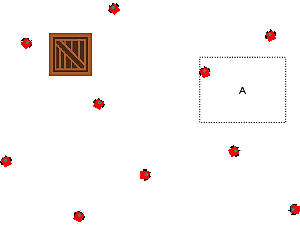
\includegraphics[width=\linewidth]{../ui_experiment/slide_images/Swarm_Robot_Control_-_10_Robot_0027.png}
		\captionof{figure}{Divide group}
		\label{fig:sub2}
	\end{minipage}
	\begin{minipage}{0.42\linewidth}
		\includegraphics[width=\linewidth]{../ui_experiment/slide_images/Swarm_Robot_Control_-_10_Robot_0029.png}
		\captionof{figure}{Combine groups}
		\label{fig:sub1}
	\end{minipage}
\end{minipage}

\begin{minipage}{\linewidth}
	\centering
	\begin{minipage}{0.42\linewidth}
		\includegraphics[width=\linewidth]{../ui_experiment/slide_images/Swarm_Robot_Control_-_10_Robot_0031.png}
		\captionof{figure}{Form a line}
		\label{fig:sub2}
	\end{minipage}
	\begin{minipage}{0.42\linewidth}
		\includegraphics[width=\linewidth]{../ui_experiment/slide_images/Swarm_Robot_Control_-_10_Robot_0033.png}
		\captionof{figure}{Form a square}
		\label{fig:sub1}
	\end{minipage}
\end{minipage}
	
	
\begin{minipage}{\linewidth}
	\centering	
	\begin{minipage}{0.42\linewidth}
		\includegraphics[width=\linewidth]{../ui_experiment/slide_images/Swarm_Robot_Control_-_10_Robot_0035.png}
		\captionof{figure}{Move the crate to A}
		\label{fig:sub1}
	\end{minipage}
	\begin{minipage}{0.42\linewidth}
		\includegraphics[width=\linewidth]{../ui_experiment/slide_images/Swarm_Robot_Control_-_10_Robot_0037.png}
		\captionof{figure}{Move the crate to A}
		\label{fig:sub2}
	\end{minipage}
	\label{fig:10_robot_slides}
\end{minipage}


\section{100 Robot Case}

\begin{minipage}{\linewidth}
	\centering
	\begin{minipage}{0.42\linewidth}
		\includegraphics[width=\linewidth]{../ui_experiment/slide_images/Swarm_Robot_Control_-_100_Robot_0003.png}
		\captionof{figure}{Move to A}
		\label{fig:sub1}
	\end{minipage}
	\begin{minipage}{0.42\linewidth}
		\includegraphics[width=\linewidth]{../ui_experiment/slide_images/Swarm_Robot_Control_-_100_Robot_0005.png}
		\captionof{figure}{Move to A with wall}
		\label{fig:sub2}
	\end{minipage}
\end{minipage}

\begin{minipage}{\linewidth}
	\centering
	\begin{minipage}{0.42\linewidth}
		\includegraphics[width=\linewidth]{../ui_experiment/slide_images/Swarm_Robot_Control_-_100_Robot_0007.png}
		\captionof{figure}{Stop the robots}
		\label{fig:sub1}
	\end{minipage}
	\begin{minipage}{0.42\linewidth}
		\includegraphics[width=\linewidth]{../ui_experiment/slide_images/Swarm_Robot_Control_-_100_Robot_0009.png}
		\captionof{figure}{Divide around obstacle}
		\label{fig:sub2}
	\end{minipage}
\end{minipage}

\begin{minipage}{\linewidth}
	\centering
	\begin{minipage}{0.42\linewidth}
		\includegraphics[width=\linewidth]{../ui_experiment/slide_images/Swarm_Robot_Control_-_100_Robot_0011.png}
		\captionof{figure}{Orange to B, Red to A}
		\label{fig:sub1}
	\end{minipage}
	\begin{minipage}{0.42\linewidth}
		\includegraphics[width=\linewidth]{../ui_experiment/slide_images/Swarm_Robot_Control_-_100_Robot_0013.png}
		\captionof{figure}{Orange to A, Red to B}
		\label{fig:sub2}
	\end{minipage}
\end{minipage}

\begin{minipage}{\linewidth}
	\centering
	\begin{minipage}{0.42\linewidth}
		\includegraphics[width=\linewidth]{../ui_experiment/slide_images/Swarm_Robot_Control_-_100_Robot_0015.png}
		\captionof{figure}{Orange to A, Red to B}
		\label{fig:sub1}
	\end{minipage}
	\begin{minipage}{0.42\linewidth}
			\includegraphics[width=\linewidth]{../ui_experiment/slide_images/Swarm_Robot_Control_-_100_Robot_0017.png}
		\captionof{figure}{Divide group}
		\label{fig:sub2}
	\end{minipage}
\end{minipage}

\begin{minipage}{\linewidth}
	\centering
	\begin{minipage}{0.42\linewidth}
		\includegraphics[width=\linewidth]{../ui_experiment/slide_images/Swarm_Robot_Control_-_100_Robot_0019.png}
		\captionof{figure}{Combine groups}
		\label{fig:sub1}
	\end{minipage}
	\begin{minipage}{0.42\linewidth}
		\includegraphics[width=\linewidth]{../ui_experiment/slide_images/Swarm_Robot_Control_-_100_Robot_0021.png}
		\captionof{figure}{Form a line}
		\label{fig:sub2}
	\end{minipage}
\end{minipage}

\begin{minipage}{\linewidth}
	\centering
	\begin{minipage}{0.42\linewidth}
		\includegraphics[width=\linewidth]{../ui_experiment/slide_images/Swarm_Robot_Control_-_100_Robot_0023.png}
		\captionof{figure}{Form a square}
		\label{fig:sub1}
	\end{minipage}
	\begin{minipage}{0.42\linewidth}
		\includegraphics[width=\linewidth]{../ui_experiment/slide_images/Swarm_Robot_Control_-_100_Robot_0025.png}
		\captionof{figure}{Move the crate to area A}
		\label{fig:sub1}
	\end{minipage}
\end{minipage}

\begin{minipage}{\linewidth}
	\centering
	\begin{minipage}{0.42\linewidth}
		\includegraphics[width=\linewidth]{../ui_experiment/slide_images/Swarm_Robot_Control_-_100_Robot_0027.png}
		\captionof{figure}{Move the crate to area A}
		\label{fig:sub2}
	\end{minipage}
	\begin{minipage}{0.42\linewidth}
		\includegraphics[width=\linewidth]{../ui_experiment/slide_images/Swarm_Robot_Control_-_100_Robot_0029.png}
		\captionof{figure}{Mark defective robot}
		\label{fig:sub1}
	\end{minipage}
\end{minipage}

\begin{minipage}{\linewidth}
	\centering
	\begin{minipage}{0.42\linewidth}
		\includegraphics[width=\linewidth]{../ui_experiment/slide_images/Swarm_Robot_Control_-_100_Robot_0031.png}
		\captionof{figure}{Remove defective robot}
		\label{fig:sub2}
	\end{minipage}
	\begin{minipage}{0.42\linewidth}
		\includegraphics[width=\linewidth]{../ui_experiment/slide_images/Swarm_Robot_Control_-_100_Robot_0033.png}
		\captionof{figure}{Patrol the screen border}
		\label{fig:sub1}
	\end{minipage}
\end{minipage}

\begin{minipage}{\linewidth}
	\centering	
	\begin{minipage}{0.42\linewidth}
		\includegraphics[width=\linewidth]{../ui_experiment/slide_images/Swarm_Robot_Control_-_100_Robot_0035.png}
		\captionof{figure}{Patrol area A}
		\label{fig:sub1}
	\end{minipage}
	\begin{minipage}{0.42\linewidth}
		\includegraphics[width=\linewidth]{../ui_experiment/slide_images/Swarm_Robot_Control_-_100_Robot_0037.png}
		\captionof{figure}{Disperse over screen}
		\label{fig:sub2}
	\end{minipage}
	\label{fig:100_robot_slides}
\end{minipage}

\section{1000 Robot Case}

\begin{minipage}{\linewidth}
	\centering
	\begin{minipage}{0.42\linewidth}
		\includegraphics[width=\linewidth]{../ui_experiment/slide_images/Swarm_Robot_Control_-_1000_Robot_0003.png}
		\captionof{figure}{Move to A}
		\label{fig:sub1}
	\end{minipage}
	\begin{minipage}{0.42\linewidth}
		\includegraphics[width=\linewidth]{../ui_experiment/slide_images/Swarm_Robot_Control_-_1000_Robot_0005.png}
		\captionof{figure}{Move to A with wall}
		\label{fig:sub2}
	\end{minipage}
\end{minipage}

\begin{minipage}{\linewidth}
	\centering
	\begin{minipage}{0.42\linewidth}
		\includegraphics[width=\linewidth]{../ui_experiment/slide_images/Swarm_Robot_Control_-_1000_Robot_0007.png}
		\captionof{figure}{Stop the robots}
		\label{fig:sub1}
	\end{minipage}
	\begin{minipage}{0.42\linewidth}
		\includegraphics[width=\linewidth]{../ui_experiment/slide_images/Swarm_Robot_Control_-_1000_Robot_0009.png}
		\captionof{figure}{Divide around obstacle}
		\label{fig:sub2}
	\end{minipage}
\end{minipage}

\begin{minipage}{\linewidth}
	\centering
	\begin{minipage}{0.42\linewidth}
		\includegraphics[width=\linewidth]{../ui_experiment/slide_images/Swarm_Robot_Control_-_1000_Robot_0011.png}
		\captionof{figure}{Orange to B, Red to A}
		\label{fig:sub1}
	\end{minipage}
	\begin{minipage}{0.42\linewidth}
		\includegraphics[width=\linewidth]{../ui_experiment/slide_images/Swarm_Robot_Control_-_1000_Robot_0013.png}
		\captionof{figure}{Orange to A, Red to B}
		\label{fig:sub2}
	\end{minipage}
\end{minipage}

\begin{minipage}{\linewidth}
	\centering
	\begin{minipage}{0.42\linewidth}
		\centering
		\includegraphics[width=\linewidth]{../ui_experiment/slide_images/Swarm_Robot_Control_-_1000_Robot_0015.png}
		\captionof{figure}{Orange to A, Red to B}
		\label{fig:sub1}
	\end{minipage}
	\begin{minipage}{0.42\linewidth}
		\includegraphics[width=\linewidth]{../ui_experiment/slide_images/Swarm_Robot_Control_-_1000_Robot_0017.png}
		\captionof{figure}{Divide group}
		\label{fig:sub2}
	\end{minipage}
\end{minipage}

\begin{minipage}{\linewidth}
	\centering
	\begin{minipage}{0.42\linewidth}
		\centering
		\includegraphics[width=\linewidth]{../ui_experiment/slide_images/Swarm_Robot_Control_-_1000_Robot_0019.png}
		\captionof{figure}{Combine groups}
		\label{fig:sub1}
	\end{minipage}
	\begin{minipage}{0.42\linewidth}
		\includegraphics[width=\linewidth]{../ui_experiment/slide_images/Swarm_Robot_Control_-_1000_Robot_0021.png}
		\captionof{figure}{Form a line}
		\label{fig:sub2}
	\end{minipage}
\end{minipage}

\begin{minipage}{\linewidth}
	\centering
	\begin{minipage}{0.42\linewidth}
		\includegraphics[width=\linewidth]{../ui_experiment/slide_images/Swarm_Robot_Control_-_1000_Robot_0023.png}
		\captionof{figure}{Form a square}
		\label{fig:sub1}
	\end{minipage}
	\begin{minipage}{0.42\linewidth}
		\includegraphics[width=\linewidth]{../ui_experiment/slide_images/Swarm_Robot_Control_-_1000_Robot_0025.png}
		\captionof{figure}{Move the crate to area A}
		\label{fig:sub1}
	\end{minipage}
\end{minipage}

\begin{minipage}{\linewidth}
	\centering
	\begin{minipage}{0.42\linewidth}
		\includegraphics[width=\linewidth]{../ui_experiment/slide_images/Swarm_Robot_Control_-_1000_Robot_0027.png}
		\captionof{figure}{Move the crate to area A}
		\label{fig:sub2}
	\end{minipage}
	\begin{minipage}{0.42\linewidth}
		\includegraphics[width=\linewidth]{../ui_experiment/slide_images/Swarm_Robot_Control_-_1000_Robot_0029.png}
		\captionof{figure}{Mark defective robot}
		\label{fig:sub1}
	\end{minipage}
\end{minipage}

\begin{minipage}{\linewidth}
	\centering
	\begin{minipage}{0.42\linewidth}
		\includegraphics[width=\linewidth]{../ui_experiment/slide_images/Swarm_Robot_Control_-_1000_Robot_0031.png}
		\captionof{figure}{Remove defective robot}
		\label{fig:sub2}
	\end{minipage}
	\begin{minipage}{0.42\linewidth}
		\includegraphics[width=\linewidth]{../ui_experiment/slide_images/Swarm_Robot_Control_-_1000_Robot_0033.png}
		\captionof{figure}{Patrol the screen border}
		\label{fig:sub1}
	\end{minipage}
\end{minipage}

\begin{minipage}{\linewidth}
	\centering	
	\begin{minipage}{0.42\linewidth}
		\includegraphics[width=\linewidth]{../ui_experiment/slide_images/Swarm_Robot_Control_-_1000_Robot_0035.png}
		\captionof{figure}{Patrol area A}
		\label{fig:sub1}
	\end{minipage}
	\begin{minipage}{0.42\linewidth}
		\includegraphics[width=\linewidth]{../ui_experiment/slide_images/Swarm_Robot_Control_-_1000_Robot_0037.png}
		\captionof{figure}{Disperse over screen}
		\label{fig:sub2}
	\end{minipage}
	\label{fig:1000_robot_slides}
\end{minipage}

\section{Unknown Number of Robots Case}

\begin{minipage}{\linewidth}
	\centering
	\begin{minipage}{0.42\linewidth}
		\includegraphics[width=\linewidth]{../ui_experiment/slide_images/Swarm_Robot_Control_-_Unknown_Number_of_Robots_0005.png}
		\captionof{figure}{Move to A}
		\label{fig:sub1}
	\end{minipage}
	\begin{minipage}{0.42\linewidth}
		\includegraphics[width=\linewidth]{../ui_experiment/slide_images/Swarm_Robot_Control_-_Unknown_Number_of_Robots_0007.png}
		\captionof{figure}{Move to A with wall}
		\label{fig:sub2}
	\end{minipage}
\end{minipage}

\begin{minipage}{\linewidth}
	\centering
	\begin{minipage}{0.42\linewidth}
		\includegraphics[width=\linewidth]{../ui_experiment/slide_images/Swarm_Robot_Control_-_Unknown_Number_of_Robots_0009.png}
		\captionof{figure}{Stop the robots}
		\label{fig:sub1}
	\end{minipage}
	\begin{minipage}{0.42\linewidth}
		\includegraphics[width=\linewidth]{../ui_experiment/slide_images/Swarm_Robot_Control_-_Unknown_Number_of_Robots_0011.png}
		\captionof{figure}{Divide around obstacle}
		\label{fig:sub2}
	\end{minipage}
\end{minipage}

\begin{minipage}{\linewidth}
	\centering
	\begin{minipage}{0.42\linewidth}
		\includegraphics[width=\linewidth]{../ui_experiment/slide_images/Swarm_Robot_Control_-_Unknown_Number_of_Robots_0013.png}
		\captionof{figure}{Orange to B, Red to A}
		\label{fig:sub1}
	\end{minipage}
	\begin{minipage}{0.42\linewidth}
		\includegraphics[width=\linewidth]{../ui_experiment/slide_images/Swarm_Robot_Control_-_Unknown_Number_of_Robots_0015.png}
		\captionof{figure}{Orange to A, Red to B}
		\label{fig:sub2}
	\end{minipage}
\end{minipage}

\begin{minipage}{\linewidth}
	\centering
	\begin{minipage}{0.42\linewidth}
		\includegraphics[width=\linewidth]{../ui_experiment/slide_images/Swarm_Robot_Control_-_Unknown_Number_of_Robots_0017.png}
		\captionof{figure}{Orange to A, Red to B}
		\label{fig:sub1}
	\end{minipage}
	\begin{minipage}{0.42\linewidth}
		\includegraphics[width=\linewidth]{../ui_experiment/slide_images/Swarm_Robot_Control_-_Unknown_Number_of_Robots_0019.png}
		\captionof{figure}{Divide group}
		\label{fig:sub2}
	\end{minipage}
\end{minipage}

\begin{minipage}{\linewidth}
	\centering
	\begin{minipage}{0.42\linewidth}
		\includegraphics[width=\linewidth]{../ui_experiment/slide_images/Swarm_Robot_Control_-_Unknown_Number_of_Robots_0021.png}
		\captionof{figure}{Combine groups}
		\label{fig:sub1}
	\end{minipage}
	\begin{minipage}{0.42\linewidth}
		\includegraphics[width=\linewidth]{../ui_experiment/slide_images/Swarm_Robot_Control_-_Unknown_Number_of_Robots_0023.png}
		\captionof{figure}{Form a line}
		\label{fig:sub2}
	\end{minipage}
\end{minipage}

\begin{minipage}{\linewidth}
	\centering
	\begin{minipage}{0.42\linewidth}
		\includegraphics[width=\linewidth]{../ui_experiment/slide_images/Swarm_Robot_Control_-_Unknown_Number_of_Robots_0025.png}
		\captionof{figure}{Form a square}
		\label{fig:sub1}
	\end{minipage}
	\begin{minipage}{0.42\linewidth}
		\includegraphics[width=\linewidth]{../ui_experiment/slide_images/Swarm_Robot_Control_-_Unknown_Number_of_Robots_0027.png}
		\captionof{figure}{Move the crate to area A}
		\label{fig:sub1}
	\end{minipage}
\end{minipage}

\begin{minipage}{\linewidth}
	\centering
	\begin{minipage}{0.42\linewidth}
		\includegraphics[width=\linewidth]{../ui_experiment/slide_images/Swarm_Robot_Control_-_Unknown_Number_of_Robots_0029.png}
		\captionof{figure}{Move the crate to area A}
		\label{fig:sub2}
	\end{minipage}
	\begin{minipage}{0.42\linewidth}
		\includegraphics[width=\linewidth]{../ui_experiment/slide_images/Swarm_Robot_Control_-_Unknown_Number_of_Robots_0031.png}
		\captionof{figure}{Patrol the screen border}
		\label{fig:sub1}
	\end{minipage}
\end{minipage}

\begin{minipage}{\linewidth}
	\centering
	\begin{minipage}{0.42\linewidth}
		\includegraphics[width=\linewidth]{../ui_experiment/slide_images/Swarm_Robot_Control_-_Unknown_Number_of_Robots_0033.png}
		\captionof{figure}{Patrol area A}
		\label{fig:sub2}
	\end{minipage}
	\begin{minipage}{0.42\linewidth}
		\includegraphics[width=\linewidth]{../ui_experiment/slide_images/Swarm_Robot_Control_-_Unknown_Number_of_Robots_0035.png}
		\captionof{figure}{Disperse over the screen area}
		\label{fig:sub1}
	\end{minipage}
\end{minipage}
\end{appendices}

\end{document}
